%% Copernicus Publications Manuscript Preparation Template for LaTeX Submissions
%% ---------------------------------
%% This template should be used for copernicus.cls
%% The class file and some style files are bundled in the Copernicus Latex Package, which can be downloaded from the different journal webpages.
%% For further assistance please contact Copernicus Publications at: production@copernicus.org
%% https://publications.copernicus.org/for_authors/manuscript_preparation.html


%% Please use the following documentclass and journal abbreviations for discussion papers and final revised papers.

%% 2-column papers and discussion papers
\documentclass[bg, manuscript]{copernicus}



%% Journal abbreviations (please use the same for discussion papers and final revised papers)


% Advances in Geosciences (adgeo)
% Advances in Radio Science (ars)
% Advances in Science and Research (asr)
% Advances in Statistical Climatology, Meteorology and Oceanography (ascmo)
% Annales Geophysicae (angeo)
% Archives Animal Breeding (aab)
% ASTRA Proceedings (ap)
% Atmospheric Chemistry and Physics (acp)
% Atmospheric Measurement Techniques (amt)
% Biogeosciences (bg)
% Climate of the Past (cp)
% DEUQUA Special Publications (deuquasp)
% Drinking Water Engineering and Science (dwes)
% Earth Surface Dynamics (esurf)
% Earth System Dynamics (esd)
% Earth System Science Data (essd)
% E&G Quaternary Science Journal (egqsj)
% European Journal of Mineralogy (ejm)
% Fossil Record (fr)
% Geochronology (gchron)
% Geographica Helvetica (gh)
% Geoscience Communication (gc)
% Geoscientific Instrumentation, Methods and Data Systems (gi)
% Geoscientific Model Development (gmd)
% History of Geo- and Space Sciences (hgss)
% Hydrology and Earth System Sciences (hess)
% Journal of Micropalaeontology (jm)
% Journal of Sensors and Sensor Systems (jsss)
% Magnetic Resonance (mr)
% Mechanical Sciences (ms)
% Natural Hazards and Earth System Sciences (nhess)
% Nonlinear Processes in Geophysics (npg)
% Ocean Science (os)
% Primate Biology (pb)
% Proceedings of the International Association of Hydrological Sciences (piahs)
% Scientific Drilling (sd)
% SOIL (soil)
% Solid Earth (se)
% The Cryosphere (tc)
% Weather and Climate Dynamics (wcd)
% Web Ecology (we)
% Wind Energy Science (wes)


%% \usepackage commands included in the copernicus.cls:
%\usepackage[german, english]{babel}
%\usepackage{tabularx}
%\usepackage{cancel}
%\usepackage{multirow}
%\usepackage{supertabular}
%\usepackage{algorithmic}
%\usepackage{algorithm}
%\usepackage{amsthm}
%\usepackage{float}
%\usepackage{subfig}
%\usepackage{rotating}
\graphicspath{{pictures/}}

\begin{document}

\title{The 2018 heatwave and its implications on ozone induced damage on vegetation in a subarctic climate}


% \Author[affil]{given_name}{surname}

\Author[1]{Stefanie}{Falk}
\Author[2]{Ane Victoria}{Vollsnes}
\Author[3]{Lisa}{Emberson}
\Author[3]{Connie}{O'Neill}
\Author[2]{Aud Else}{Berglen Eriksen}
\Author[1]{Bj{\o}rg}{Rognerud}
\Author[1]{Frode}{Stordal}
\Author[1]{Terje}{Koren Berntsen}

\affil[1]{Department of Geosciences, University of Oslo, Oslo, Norway}
\affil[2]{Department of Biosciences, University of Oslo, Oslo, Norway}
\affil[3]{Department of Environment and Geography, University of York, UK}
%% The [] brackets identify the author with the corresponding affiliation. 1, 2, 3, etc. should be inserted.

%% If an author is deceased, please mark the respective author name(s) with a dagger, e.g. "\Author[2,$\dag$]{Anton}{Aman}", and add a further "\affil[$\dag$]{deceased, 1 July 2019}".

%% If authors contributed equally, please mark the respective author names with an asterisk, e.g. "\Author[2,*]{Anton}{Aman}" and "\Author[3,*]{Bradley}{Bman}" and add a further affiliation: "\affil[*]{These authors contributed equally to this work.}".


\correspondence{Stefanie Falk (stefanie.falk@geo.uio.no)}

\runningtitle{2018 heatwave and implication on ozone induced damage on vegetation in subarctic climate}

\runningauthor{Falk et al.}





\received{}
\pubdiscuss{} %% only important for two-stage journals
\revised{}
\accepted{}
\published{}

%% These dates will be inserted by Copernicus Publications during the typesetting process.


\firstpage{1}

\maketitle


\begin{abstract}
  The summer 2018 and summer 2019 did not differ significantly in the level of ozone. On the other hand, the temperatures (precipitation and cloud cover/PAR?) differed quite a lot. We also observed ozone-induced visible injuries on clovers in the ozone garden at Svanhovd in 2018, but not in 2019. This may be due to differences in uptake of ozone ($\mathrm{POD_y}$) between the two years. Since DO3SE can be run on birch/beech and conifers, we would like to investigate whether the critical levels for these tree species were crossed during the two summer seasons. Ozone concentrations for the two missing weeks in July 2018 have been estimated based on the measurements from the Swedish and Finnish ozone measurement stations in the region.  
\end{abstract}


\copyrightstatement{TEXT}


\introduction  %% \introduction[modified heading if necessary]
\label{sec:intro}

%{\bf OBS: The following is just a copy of the 2018 dry deposition paper. It has to be substantially changed to meet the no-copycat-criteria. TODO: Rewrite in context of this article.}

%Ozone is an important trace gas for all lifeforms on Earth. Depending on the place of its occurrence it has either a positive or negative connotation. In the stratosphere, ozone absorbs most of the ultraviolet (UV)-light from the sun within the range of 100--315\,\unit{nm}, thus shielding the Earth's surface from the most harmful UV-radiation. In addition, ozone is a potent greenhouse gas in both, stratosphere and troposphere. With a radiative forcing of $0.40 \pm 0.20\,\unit{W\,m^{-2}}$, it is placed third, only surpassed by \chem{CO_2} and \chem{CH_4} \citep[Chapter 8]{IPCC2013}.\\
%In the troposphere and in particular in ambient air, ozone is considered as a highly toxic pollutant. Since the industrial revolution, tropospheric background ozone concentrations have been increasing in the northern hemisphere \citep[Chapter 2]{IPCC2013}. In recent years, the number of episodes of peak concentrations has been, in general, decreasing in North America and Europe due to the implementation of air quality regulations \citep[e.g.,][]{ESA:Fleming2018, ESA:Mills2018}. At the same time, fast developing countries, like e.g., China or India, saw a significant increase in ozone related air pollution. Continuously high concentrations of ambient air ozone are hazardous to the whole ecosystem. It is estimated that ozone is cause to an increase in pre-mature deaths \citep{WHO2008}, an average global loss of yield in the four major crops (wheat, rice, maize, and soybean) of about $3-15\,\unit{\%}$ \citep{PJ:Ainsworth2017} as well as $7\,\unit{\%}$ loss in primary production in forestry \citep{GCB:Wittig2009,EP:Matyssek2012}. The impact of ozone damage on vegetation and agricultural plants may affect food security in the future especially in Asia \citep{GCB:Tang2013,NCC:Tai2014,AE:Chuwah2015,GCB:Mills2018} and might be an important additional feedback to climate change \citep{Nat:Sitch2007}.\\
%Elevated ozone levels at a site may originate from both, the local production of ozone from its precursors, which are transported, and from advection of ozone itself. Long-range ozone transport occurs regularly and might be most important in regions that otherwise lack precursors. Tropospheric ozone is produced in complex photochemical cycles involving precursor gases such as carbon monoxide (\chem{CO}) or volatile organic substances (VOCs -- also known as hydrocarbons) in the presents of nitrogen oxides (\chem{NO_x}). A typical reaction mechanism for \chem{CO} is sketched in the following. In a sequence of rapid reactions a peroxyl radical \chem{HO_2^\bullet} is formed through an initial reaction of \chem{CO} with a hydroxyl radical \chem{^\bullet OH}.
%Via a reaction between \chem{HO_2^\bullet} and \chem{NO}, \chem{NO_2} is formed which is then photolyzed. The resulting atomic oxygen reacts then with \chem{O_2} (and also under the presence of available co-reactants) to form an ozone molecule.

%Since ozone is highly reactive, its global mean life-time in the troposphere is roughly $22$ days but ranges between a few days in the tropical boundary layer to up to $1$ year in the upper troposphere \citep{JGR:Stevenson2005,ACP:Young2013}. The abundance of tropospheric ozone therefore varies, e.g., with time of the day, season, altitude, location \citep{ACP:Schnell2015}, or weather conditions in general \citep{ACP:Otero2018}. Typical concentrations of surface ozone range from $10\,\unit{ppb}$ over the tropical Pacific to $100\,\unit{ppb}$ in the downwind areas of highly emitting sources \citep[Chapter 8]{IPCC2013}. This variability poses a challenge on both, trend analysis from observations as well as validation and inter-comparison of models. From the observational side, the number of long-term observations (started before the 1950s) is limited and restricted to mainly European sites. Most of these indicate a doubling of tropospheric ozone since the 1950s \citep[Chapter 2]{IPCC2013}.

{\bf TODO:
\begin{itemize}
\item general about ozone $\rightarrow$ focus on surface ozone and in particular precursors with respect to the forest fires (\chem{CO}) and heat stress (\chem{VOCs}).
\item ozone induced damage in vegetation \emph{Contributor: Ane - maybe also ask Aud?}\\
  Ozone acts as an oxidative stress to plants. Its main action is imposed through reactions occurring in the cell walls and cell membranes of mesophyll cells inside the leaves. Ozone enters the leaves through stomata, that are kept open to allow for gas exchange between the leaf air spaces and the exterior air. When the stomata are closed, ozone does not enter.
\item[$\rightarrow$] Some info on stomatal conductance and its empirical calculation:
  \begin{equation}
  g^k_\text{sto, m} = g^k_\text{max, m} \cdot f^k_\text{phen} \cdot f^k_\text{light} \cdot \max{\left\{f^k_\text{min}, f^k_T \cdot f^k_D \cdot f^k_\text{SW}\right\}}.
  \label{eq:stomatal}
\end{equation}
%
The factors herein are normalized and vary within the range $0-1$. They account for leaf phenology ($f_\text{phen}$), light ($f_\text{light}$), temperature ($f_T$), water vapor pressure deficit ($f_D$), and soil water content ($f_\text{SW}$). All factors differ with plant functional type $k$.
\item metrics of ozone
  \begin{itemize}
  \item[$\rightarrow$] Concentration based
    \begin{equation}
      \mathrm{AOT_x} = \int{\mathrm{max(\chem{[O_3]}-x)}\cdot \mathrm{dt}},
    \end{equation}
    with the ambient ozone concentration $\chem{[O_3]}$ and the concentration threshold $\mathrm{x}$. A typical value for $\mathrm{x}=40\,\unit{ppb}$.
  \item[$\rightarrow$] Flux based
    \begin{equation}
      \mathrm{POD_y} = \int{\mathrm{max(\Phi_\chem{[O_3]}-y)}\cdot \mathrm{dt}},
    \end{equation}
    with the ambient ozone flux through the stomata $\Phi_\chem{[O_3]} = g_\mathrm{sto} \cdot \chem{[O_3]}$ and the flux threshold $\mathrm{y}$.
  \end{itemize}
\item present subarctic climate and conditions
  \begin{itemize}
  \item[$\rightarrow$] midnight sun and 23\,\unit{h} open stomata (biological details will be published in a component paper)
  \item[$\rightarrow$] ozone climatology and spring peak \citep{AE:Monks2000, AB:Klingberg2009, AE:Rummukainen1996} {\bf TODO: Find newer articles.}
  \end{itemize}
\end{itemize}
}

Following a report by the Norwegian Meteorological institute \citep{MetNOR2019}, the summer of 2018 was the warmest and driest ever recorded in eastern, western, and southern Norway. In the north (including Finnmark), it was amongst the warmest on record - favorable conditions for boundary layer ozone formation.

An unusually weak and northward shifted jet stream allowed for a persistent high pressure system above northern Europe, including Fennoscandia which blocked the pressure systems for several consecutive months. In the period May -- July, southern Norway had temperatures $4\,\unit{^\circ C}$ above normal. While southern Norway had only about $60\,\unit{\%}$ of normal precipitation, northern Norway as a whole had close to normal precipitation, but with local variations.

Heat and drought stress on vegetation was exceptional not only in large parts of Fennoscandia but also in much of Europe, where the influence of the high pressure system extended even over a period of five months (April/May, July--September). These conditions gave rise to massive forest fires in different parts of Europe and thus an increase in ozone precursors (\chem{CO}, \chem{VOCs}).

A total of 2079 forest fires of different size were registered in Norway in 2018, twice as many as in the preceding years 2016/17 \citep{DSB2019}, last accessed April 2020). In Sweden, about 500 fires had been reported (five times more than in a usual summer) and an estimated total of $25000\,\unit{hectare}$ burned down in the course of the most extensive fires in central Sweden (G\"{a}vleborgs, J\"{a}mtlands, and Dalarnas l\"{a}n) in younger history \citep{SOU2019}.

Elevated ozone in Europe was likely due to several other factors as well, like in the 2003 drought period, such as biogenic VOC emissions, reduced dry deposition, reduced clouds and increased solar radiation, photochemical reactions, and stagnant weather conditions \citep{JGR:Solberg2018}.\\

{\bf TODO: Future climate and conditions
  \begin{itemize}
  \item[$\rightarrow$] increase in heatwaves and dry periods
  \item[$\rightarrow$] shift in start of growing season (into vicinity of ozone spring peak) \citep{GCB:Menzel2006,RS:Hogda2013}
  \item[$\rightarrow$] increase in tropospheric background ozone
  \end{itemize}
}

In terms of AOT40, the threshold for protection of vegetation of $3000\,\unit{ppb}$ given by the EU directive has been well exceeded at many ozone monitoring sites in Southern Norway in the 2018 growing season \citep{NILU2019}. {\bf TODO: come back to this later on in the discussions(?) - it has not been breached at Svanvik in northern Fennoscandia. Later supplement figure \ref{fig:fennoscandic_aot40}}

Within the scope of our project to assess probable effects of midnight sun conditions on ozone uptake by plants and resultant enhanced susceptibility to ozone inflicted damage, we conducted ambient air ozone concentration measurements at Svanhovd in the growing seasons of 2018/19 in collaboration with NILU. 
In 2018, we have observed ozone damage on semi-natural vegetation (clover) and crops (tobacco) in the ozone garden at NIBIO Environment Centre Svanhovd. In contrast, no such damage was found on the clovers in 2019, although it was found on the sensitive tobacco cultivar. This indicates that the vegetation may have been more affected by ozone in 2018 than in 2019.
The respective observed average ozone concentration in 2018/19, however, did not differ significantly by statistical means.

As previously mentioned, ozone damage is rather driven by the actual uptake of ozone ($\mathrm{POD_y}$) than by the accumulated ambient air concentration above a certain threshold ($\mathrm{AOT_x}$). Through the stomatal conductance, $\mathrm{POD_y}$ depends on environmental drivers such as ambient air temperature, photoactive radiation, soil water availability, and water vapor pressure deficit.

In this study, we investigate potential main drivers for the observed ozone damage in the growing season 2018 at NIBIO Environment Centre Svanhovd in contrast to 2019. We compare $\mathrm{POD_y}$ values for natural and semi-natural vegetation for derived climatological averages of environmental conditions at Svanhovd as well as for the growing seasons 2018/19 which shall serve as case studies.

The observation site at NIBIO Environment Centre Svanhovd and all related data are presented in Section~\ref{sec:data}. In Section~\ref{sec:stats}, we derive climatologies for surface ozone concentration at Svanhovd and northern Fennoscandia based on in situ observations and also compute climatologies of surface temperature, precipitation, and global radiation for Svanhovd. Based on these, we evaluate anomalies of environmental key variables in 2018/19 by statistical means. In addition, the derived surface ozone concentration climatology for northern Fennoscandia will be compared with available ozone reanalysis products. We use the DO3SE model to estimate the ozone uptake by natural and semi-natural vegetation to investigate the main environmental driver of the observed ozone damage in 2018 (Section~\ref{sec:do3se}). In Section~\ref{sec:conc} finally, we will summarize our results, draw conclusions, and give an outlook on further work.


\section{Data}
\label{sec:data}

In our assessment of ozone damage on vegetation in the subarctic in relation to the 2018 heatwave, we focus on the NIBIO operated Environment Centre Svanhovd which lies close by the settlement of Svanvik in the Pasvik valley (Section~\ref{subsec:svanhovd}). Throughout the paper, we will use Svanhovd synonymously for the atmospheric monitoring site at Svanvik. The available meteorological monitoring data are described in Section~\ref{subsubsec:atmo_svanvik}. In Section~\ref{subsubsec:ozone_garden}, the ozone garden -- a plant-based ozone monitoring -- will be described in more detail. Other data used for evaluation of the ozone data taken at Svanhovd is described in Section~\ref{subsec:other_data}. We compare with observational data from other monitoring sites in northern Fennoscandia (Section~\ref{subsubsec:ebas}) and use as well reanalysis products (Section~\ref{subsubsec:ozone_rea}) as complement when observational data was not available.

\subsection{NIBIO Environment Centre Svanhovd}
\label{subsec:svanhovd}
"Svanhovd is located beside the Pasvik river, in the middle of the wedge of Norwegian land separating Russia and Finland in the north. It is where the eastern Siberian taiga meets the western Boreal forest. [...] Svanhovd was originally established as a State Demonstration and Experimental Farm in the 1930's, in order to expand agriculture in Pasvik valley [...]" - \href{https://www.nibio.no/en/about-eng/addresses/northern-norway/svanhovd}{NIBIO web page, accessed March 2020}.

The locations of the atmospheric monitoring site as well as the ozone garden with respect to the main buildings of the Svanhovd Environment Centre are marked in the aerial photography shown in Fig.~\ref{fig:svanhovd_research_station}. The Centre is located south of the settlement of Svanvik, where as the border to Russia, the Pasvik river, lies only a few hundred meters to the east. The original farm buildings, protected by law, are located in the lower center, while the Svanhovd Environment Centre follows to the north-east. Left of the Centre and north of the original farm buildings a botanical garden can be found. It is one amongst three such gardens north of the Polar Circle. The Svanhovd Environment Centre focuses on research of the special environment of the region, but also comprises long-term observations of various agrometeorological variables, i.a. $2\,\unit{m}$ temperature, precipitation, global irradiance, and soil temperature at different depths.

For the purpose of relating observed damage on ozone sensitive plants (e.g. clover and tobacco) to local ozone concentrations, an ozone monitor had been installed during the growing seasons 2018/19. The relevant data are described in more detail in Section~\ref{subsubsec:atmo_svanvik}.

\emph{Comment: Invite co-authors from NILU and NIBIO?}

\begin{figure}[t]
  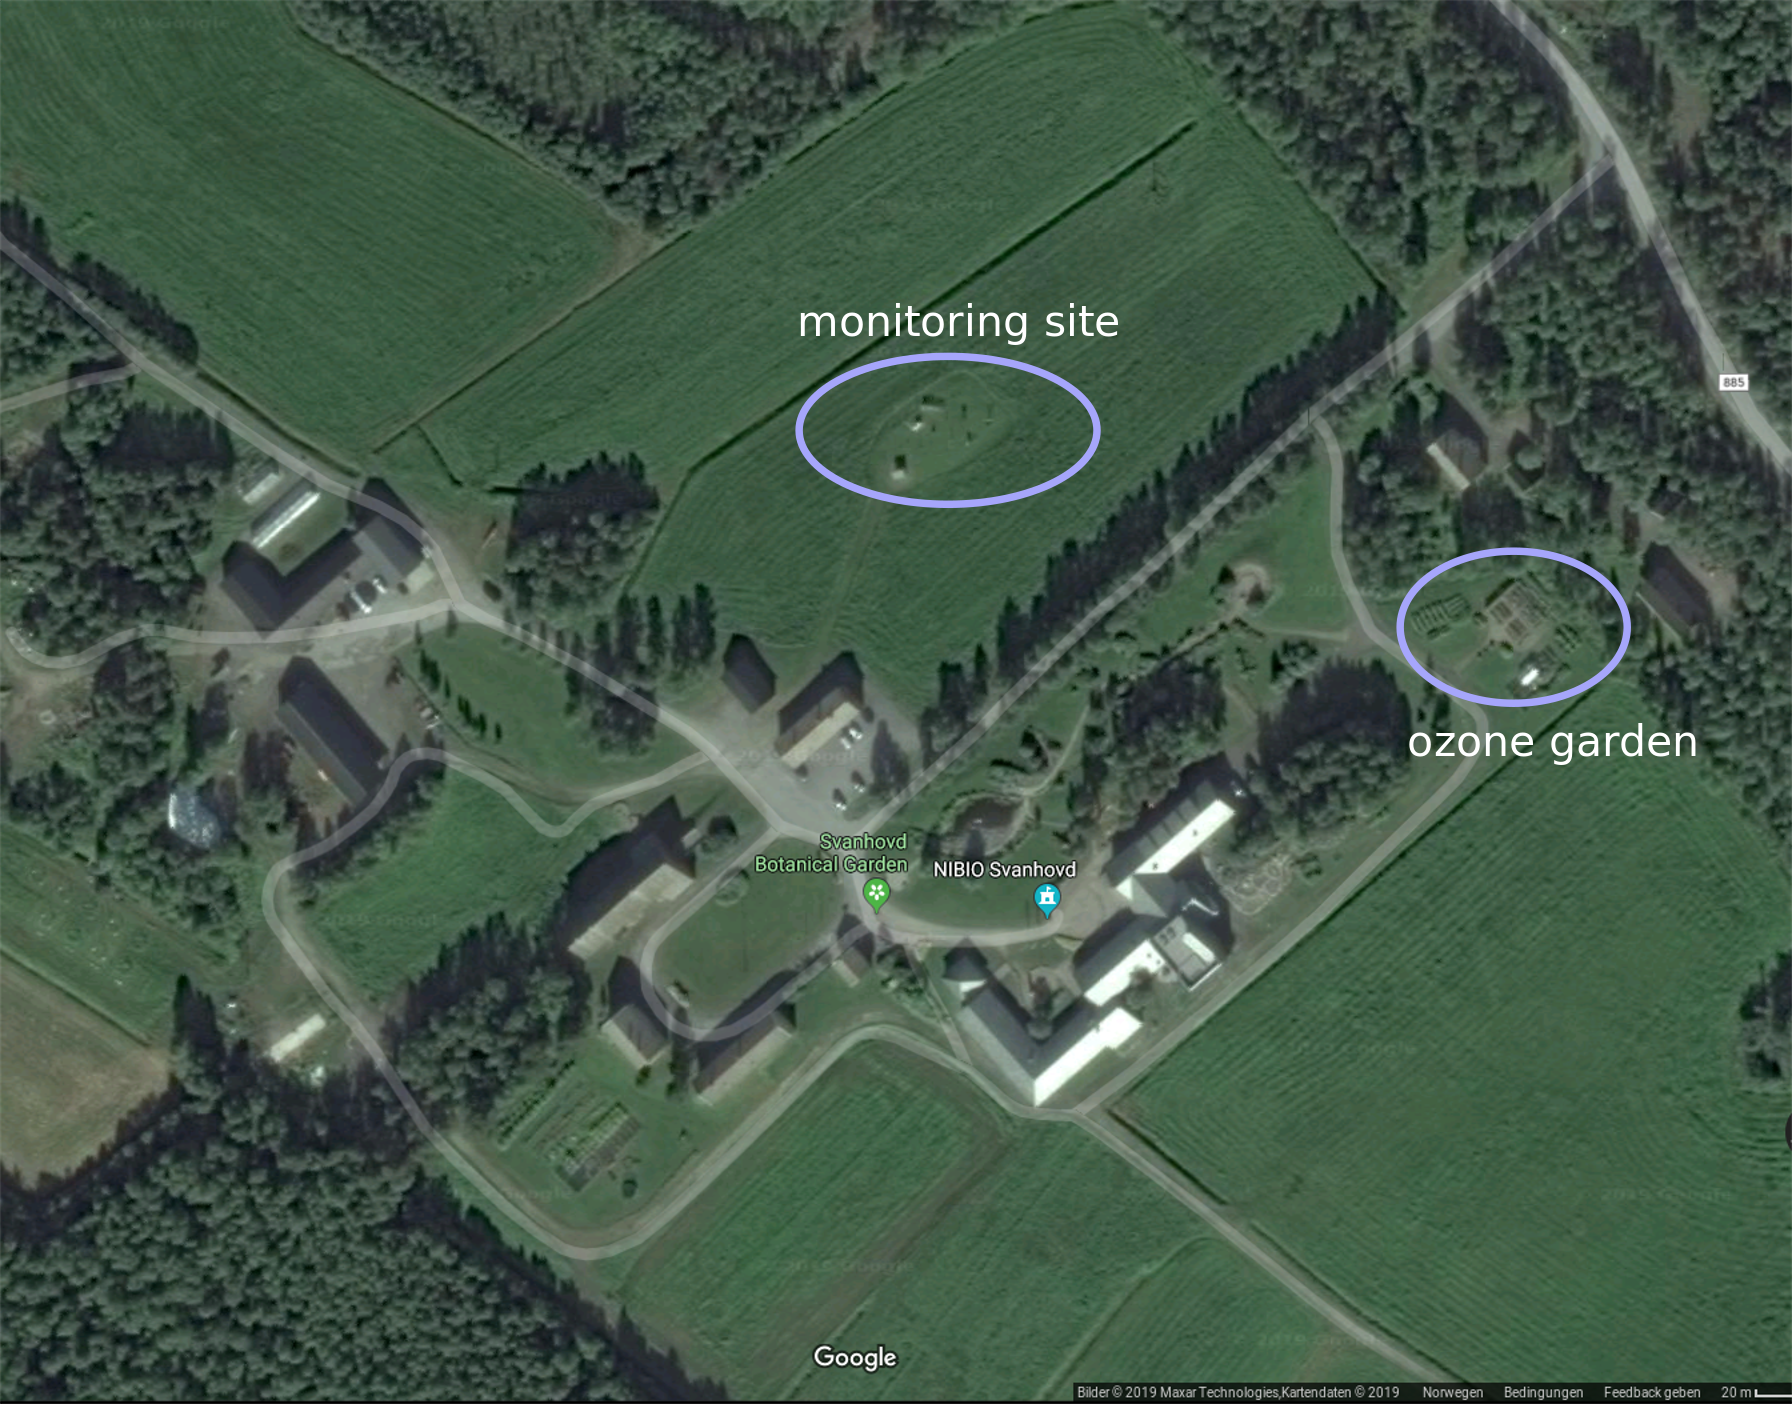
\includegraphics[width=8.3cm]{svanhovd_researchstation}
  \caption{NIBIO Environment Centre Svanhovd close by the settlement of Svanvik, Norway. Atmospheric monitoring site and ozone garden have been marked. Aerial photography \copyright Norges Kartverk.}
  \label{fig:svanhovd_research_station}
\end{figure}


\subsubsection{Atmospheric monitoring}
\label{subsubsec:atmo_svanvik}
For the growing seasons 2018/19, monitoring data of key variables (temperature, precipitation, and ozone) have been downloaded from \href{luftkvalitet.no}{luftkvalitet.no} which is operated by NILU.

All agrometeorological variables including temperature and precipitation are available from September 1992 to present day (LandbruksMeteorologisk Tjeneste provided by NIBIO -- \href{https://lmt.nibio.no/}{lmt.nibio.no}, note the station name here is Pasvik).

{\bf TODO: Some more (technical) details about ozone and atmospheric monitoring at Svanhovd? $\rightarrow$ Sverre?}

\emph{Comment: We refrain from doing a full cross-evaluation for these meteorological fields, since this has been done elsewhere. It's somewhat clear that this is a job of the operators in the monitoring network \citep{MetNOR2019}.}

Relevant data for the growing season 2018/19 are shown in Fig.~\ref{fig:data_svanvik_2018_2019}. The hatched areas mark times when no ozone data was recorded. Note, while the downtime during winter was planned, missing data in two weeks of July 2018 (July 9--23) were due to problems in data acquisition.

Ozone concentrations \chem{[O_3]} measured in $2\,\unit{m}$ height above ground are averaged hourly. As can be seen in Fig.~\ref{fig:data_svanvik_2018_2019}a), \chem{[O_3]} peaks in spring (April/May) and reaches its minimum in late summer (July/August). The spring peak has not been captured completely in 2019, for data acquisition started later than in 2018. In summer 2018 (June--August), high ozone concentrations ($\chem{[O_3]} > 40\,\unit{ppb}$) were recorded 50 times. The highest summer ozone concentration ($\chem{[O_3]} = 50.2\,\unit{ppb}$) was measured on July 25. This coincides with the period of the most extensive forest fires in central Swedish (G\"{a}vleborgs, J\"{a}mtlands, and Dalarnas l\"{a}n) which occurred from July 12--29 and destroyed about $18000\,\unit{hectare}$ of forest \citep{SOU2019}. {\bf TODO: Do we need a corresponding \chem{CO_2} emission here?} However, due to the above mentioned data acquisition problems, we missed most of the corresponding ozone data for this event and most likely also the peak ozone concentration. In contrast, ozone concentration only rose 18 times above the threshold of $40\,\unit{ppb}$ during the summer of 2019.

Hourly averaged $2\,\unit{m}$ temperatures below $-20\,\unit{^\circ C}$ were observed in winter (January/February), while high temperatures (above $20\,\unit{^\circ C}$) occurred in summer (July), though more regularly in 2018 than in 2019 (Fig.~\ref{fig:data_svanvik_2018_2019}b). In 2018, temperature regularly rose above freezing only in May, while in 2019 this occurred already early in March/April. 2019 saw a very cold November with temperatures regularly below $-10\unit{^\circ C}$.

More rain events with accumulated daily precipitation $\sum_d \mathrm{Precip}$ above $10\,\unit{mm}$ occurred in the summer of 2018 compared to 2019 (Fig.~\ref{fig:data_svanvik_2018_2019}c). $\sum_d \mathrm{Precip} \ge 20\,\unit{mm}$ was only breached twice in 2018 and once in 2019.

In 2018, global irradiance $Q_0$ (Fig.~\ref{fig:data_svanvik_2018_2019}d) displays more sequentially high values in spring (May) and summer (July) compared to 2019, while June 2019 saw more consecutive high irradiance than 2018. In both years, the maximum recorded $Q_0$ was roughly $750\,\unit{W\,m^{-2}}$ reached only in June.

\begin{figure*}[t]
  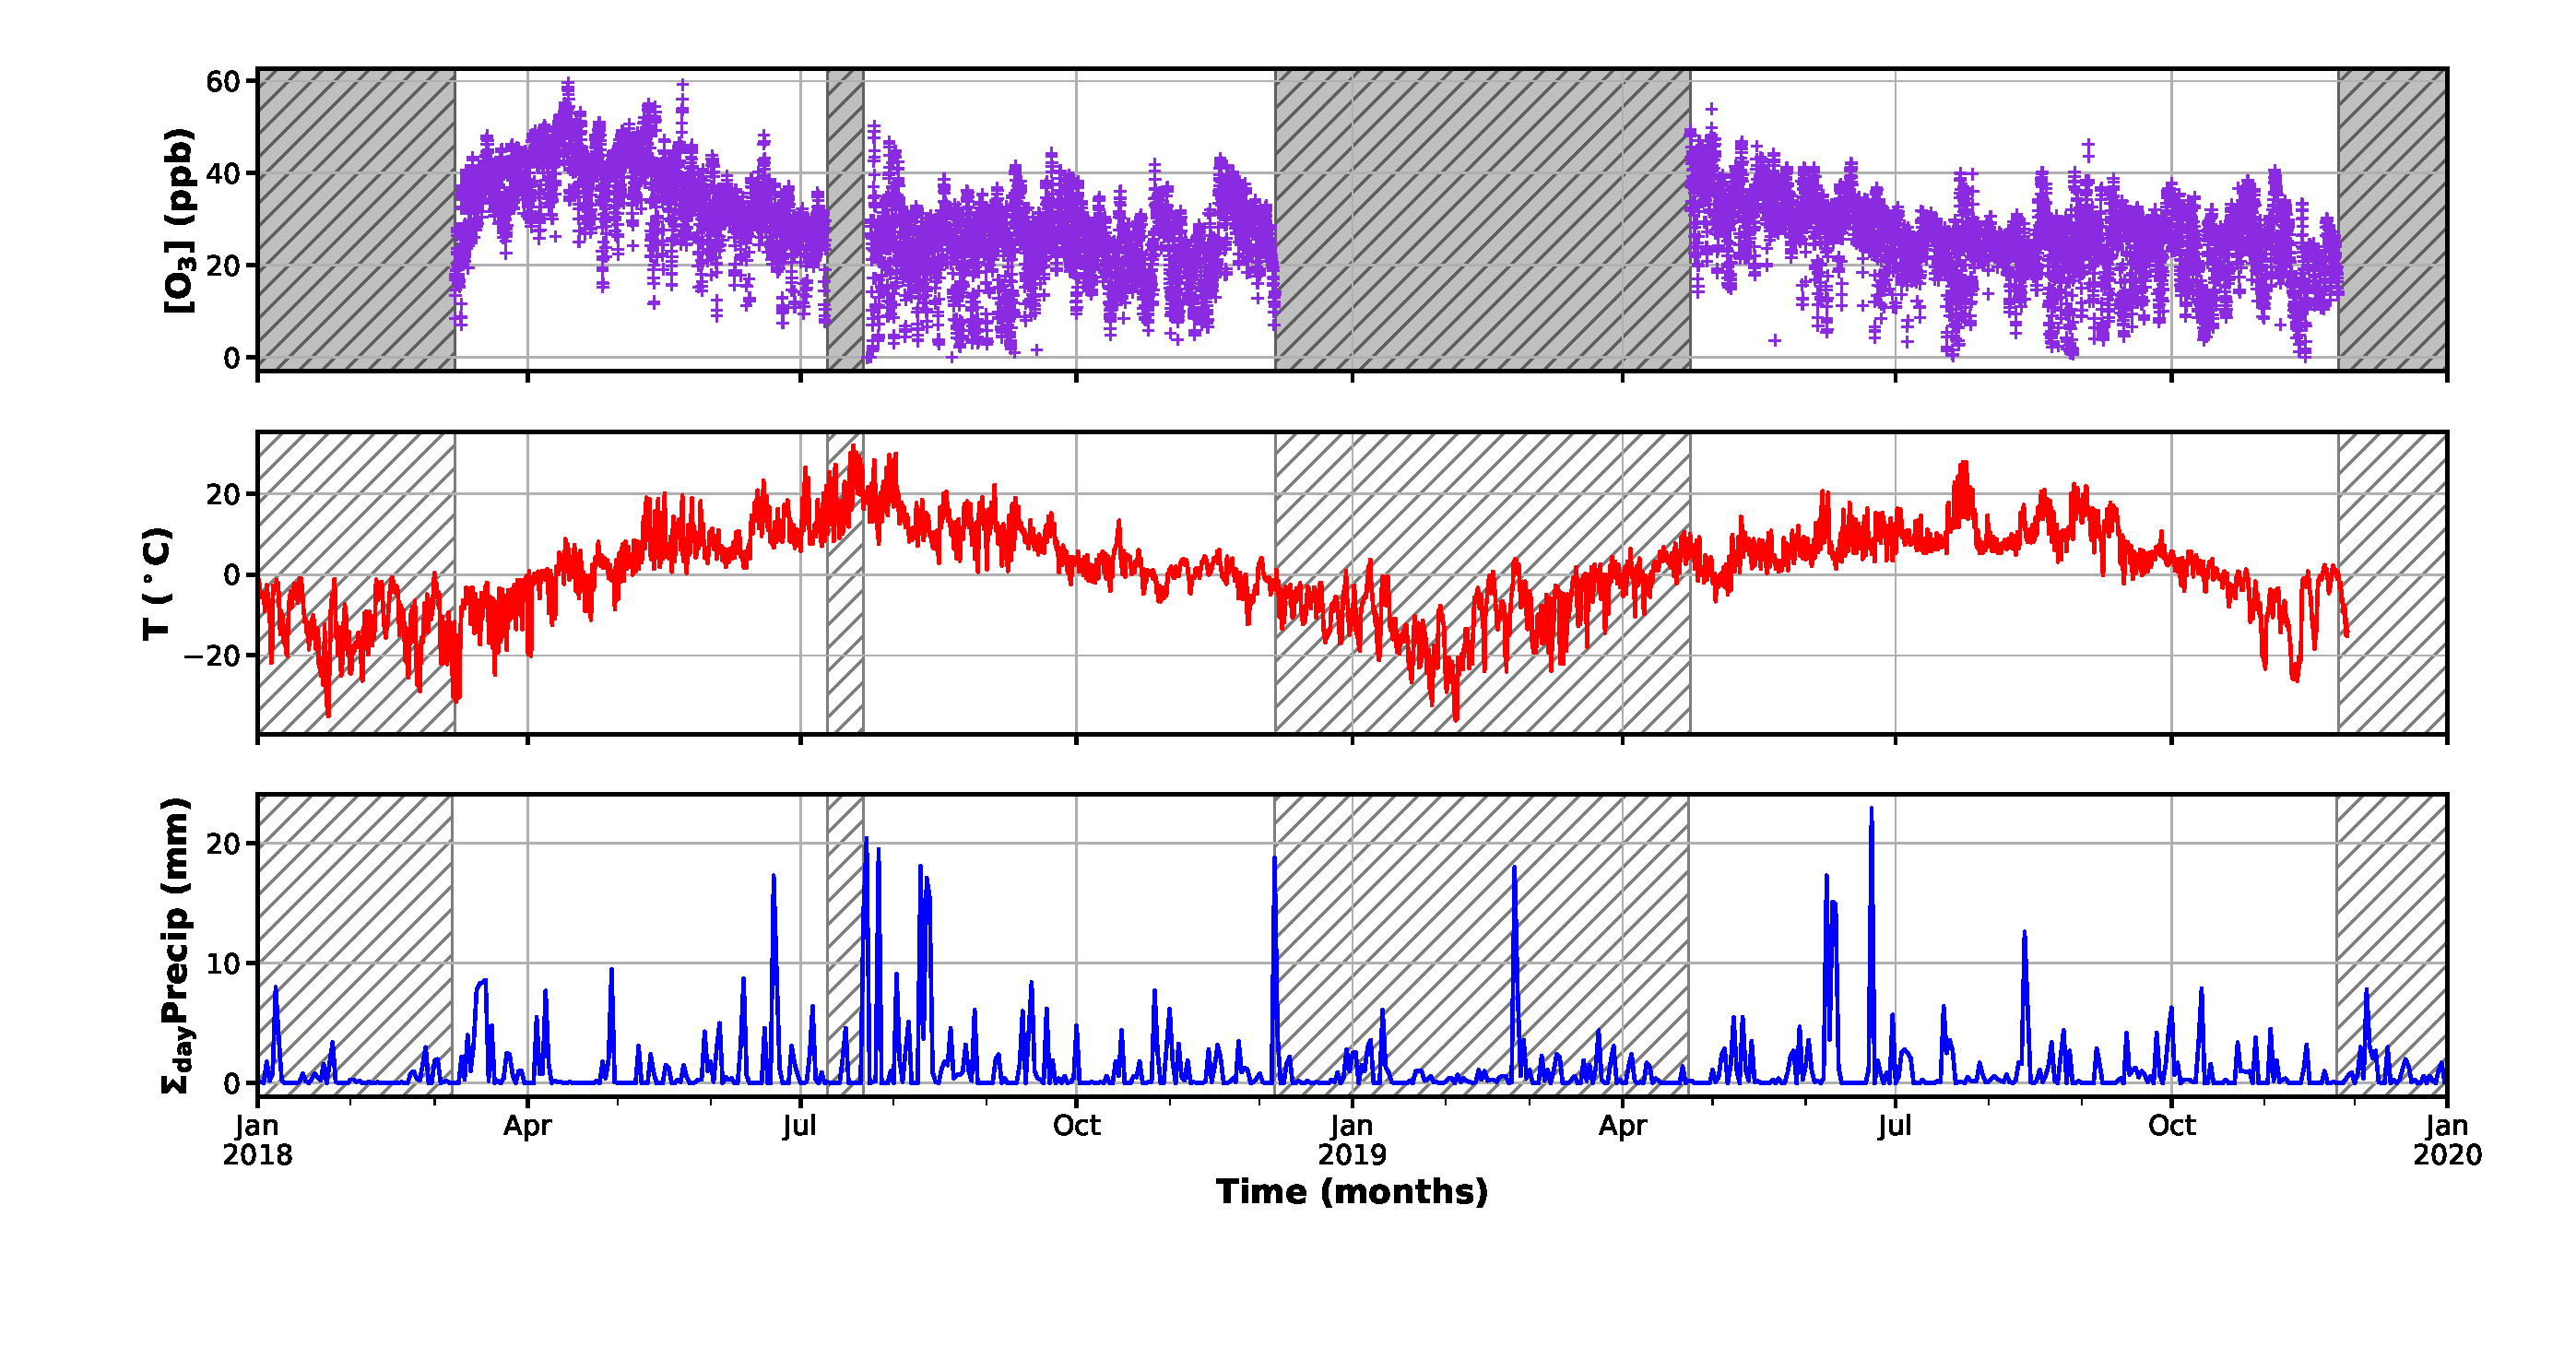
\includegraphics[width=12cm]{data_svanvik_2018_2019}
  \caption{Observational data from atmospheric monitoring at Svanhovd in 2018/19. The hatched areas indicate missing ozone monitoring data. (a) Hourly averaged ozone concentration; (b) hourly averaged temperature; (c) daily accumulated precipitation; (d) hourly averaged global irradiance.}
  \label{fig:data_svanvik_2018_2019}
\end{figure*}


\subsubsection{Ozone garden}
\label{subsubsec:ozone_garden}
      {\bf TODO: Details about the ozone garden and observed damage on ozone sensitive plants. We will need to come back to this in the discussion section after the Do3se modeling part.} \emph{Author: Ane/Aud -- pictures are welcome, just upload them on overleaf or send them to me.}



\subsection{Other data}
\label{subsec:other_data}
To determine the significance of the ozone conditions in 2018, we have to derive a surface ozone concentration climatology for Svanvik. From 1986--1996 ozone monitoring has been operated by NILU at Svanhovd, but no ozone measurements have been conducted for the past $14\,\unit{years}$. Due to probable changes in northern hemispheric tropospheric background ozone and a reduction of summertime peak values related to ozone precursors that fell under air quality regulations {\bf TODO: Citations!}, we also have to have a look at ozone observations at other sites in northern Fennoscandia. In regard to ozone, available observational data are sparse in this region. An overview over the geographical locations of conducted atmospheric monitoring in the past and present is given in Fig.~\ref{fig:station_map_fennoscandia}. The data is described in Section~\ref{subsubsec:ebas}. 
As additional complement to observational data which is not available at all times and spatially sparse, we also look at various ozone reanalysis products (Section~\ref{subsubsec:ozone_rea}).

\begin{figure}[t]
  \includegraphics[width=8.3cm]{station_map_fennoscandia}
  \caption{Cap of the North. Locations of past and present ozone observation sites in northern Fennoscandia used within this study. For more details see Tab.~\ref{tab:ebas_obs}. The same color coding for each station as displayed herein will be used in all following figures.}
  \label{fig:station_map_fennoscandia}
\end{figure}

\subsubsection{Surface ozone observations}
\label{subsubsec:ebas}
All surface ozone observations used in this study are available from the EBAS database operated by NILU (\href{http://ebas.nilu.no/}{ebas.nilu.no}). In Table~\ref{tab:ebas_obs}, we give an overview over the exact locations and time range of operational data taking. All stations with available long term observations are located on higher ground than Svanhovd which will result in higher surface ozone concentrations in comparison as ozone abundance, in general, decreases with decreasing altitude in the absence of local precursors. {\bf TODO: Citation see references in \citet{AB:Klingberg2009}!} {\bf TODO: The following has to be confirmed and elaborated on! Ane?} The vegetation at all sites is similar and consists mainly of pine forests, birch, and heath.

Data from before the 1990s is available solely from Svanvik and Karasjok. These data, however, do not follow the high quality standard procedures implemented nowadays and have to be treated with care \citep{NILU2003}. Especially, ozone monitors did not undergo a regular re-calibration. This probably leads to drifts in the observed data and may impose a false periodicity. In 1997, the ozone monitoring at Jergul was relocated downstream the river Karasjokka to a site close by Karasjok. Although the same equipment has been used, this might have introduced a breaking point in the combined data series, denoted as Jergul/Karasjok in the following, which would be of a problem if this was the sole data to compare with. Only few data have been taken upstream the Pasvik river at Janiskovski, hence these will not be taken into further consideration, but are shown for completion. As can be seen in Fig.~\ref{fig:ozone_timesseries_fenoscandic_obs}, there is an overlap of about $4\,\unit{years}$ between data taken at Esrange, Jergul/Karasjok, and Svanvik. The hatched areas indicate time periods with insufficient quality control as mentioned above.

\begin{table}[t]
  \caption{Past and present ozone observation sites in northern Fennoscandia. Data available on \href{http://ebas.nilu.no/}{EBAS}.}
  \label{tab:ebas_obs}
  \begin{tabular}{lllllrl}
    \tophline
    Name       & Country & ID      & \multicolumn{3}{c}{Location} & Operational\\
    &         &         & lat             & lon               & alt            &\\
    &         &         & (\unit{^\circ N}) & (\unit{^\circ E})  & (\unit{m})     &\\
    \middlehline
    Esrange    & SWE     & SE0013R & 67.83           & 21.07             & 475            & 1991 -- present\\
    Janiskoski & RUS     & RU0001R & 68.93           & 28.85             & 118            & 1995 -- 1997\\
    Jergul     & NOR     & NO0030R & 69.45           & 24.60             & 255            & 1997 -- 2011\\
    Karasjok   & NOR     & NO0055R & 69.467          & 25.217            & 333            & 1988 -- 1997\\
    Pallas     & FIN     & FI0096G & 69.97           & 24.12             & 565            & 1995 -- present\\
    Svanvik    & NOR     & NO0047R & 69.45           & 30.03             & 30             & 1986 -- 1996$^\dagger$\\
    \bottomhline
  \end{tabular}
  \belowtable{$^\dagger$ Exclusive ozone monitoring growing seasons 2018/19 operated by NILU.} % Table Footnotes
\end{table}


\begin{figure*}[t]
  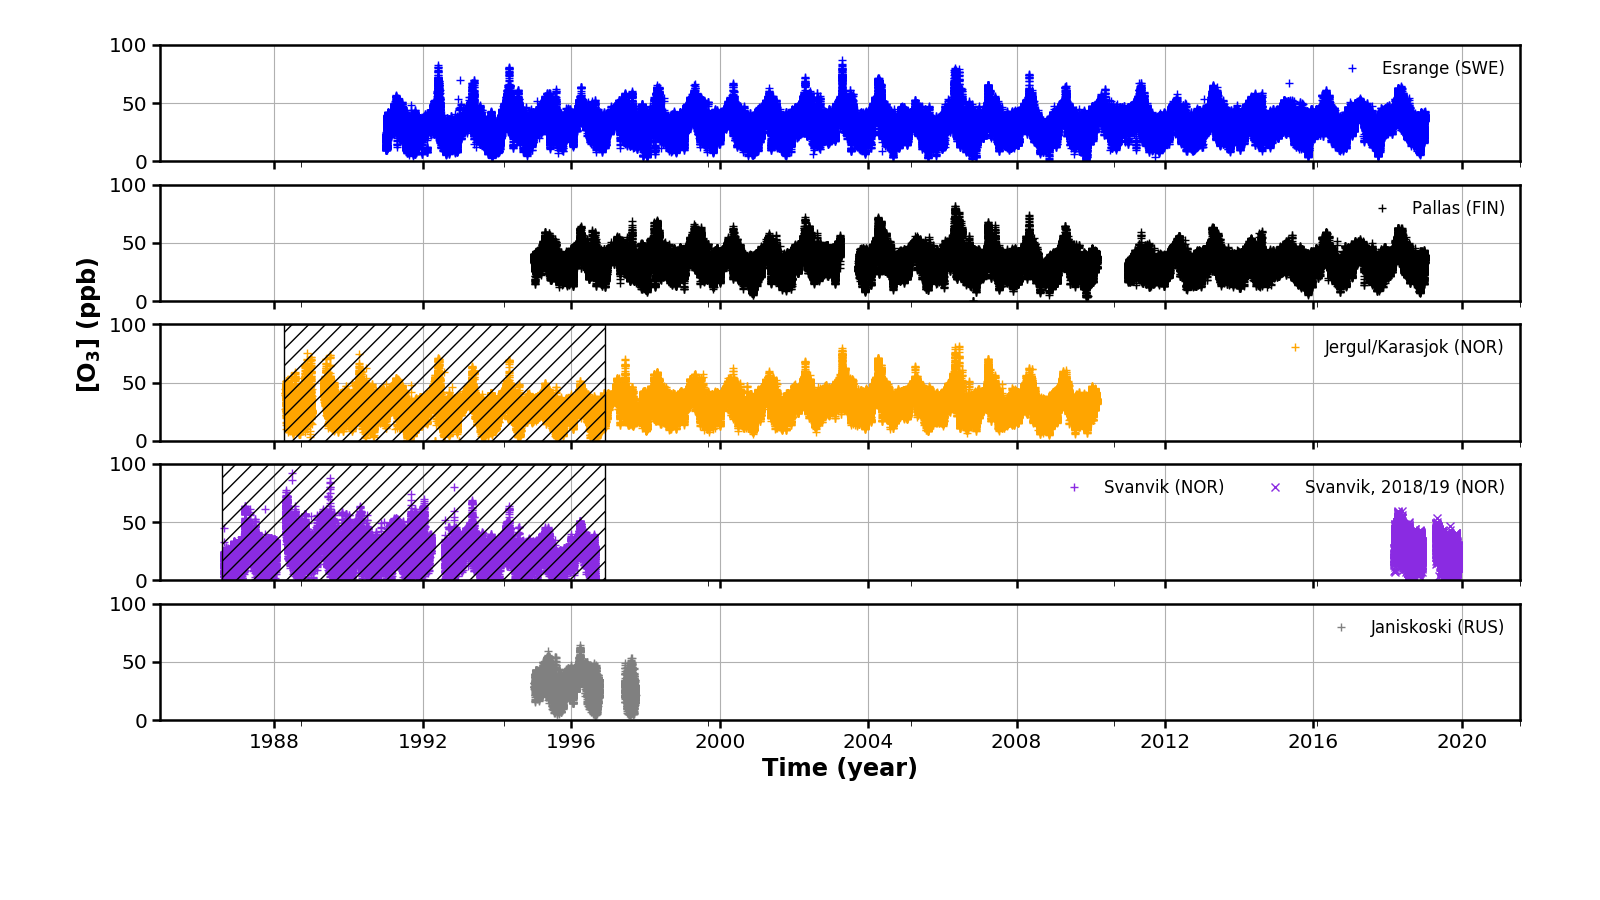
\includegraphics[width=12cm]{ozone_timeseries_fenoscandic_obs.png}
  \caption{Time series of ozone observations in northern Fennoscandia (Tab.~\ref{tab:ebas_obs}). Data taken from EBAS. The hatched areas indicate time periods with insufficient quality control \citep{NILU2003}.}
  \label{fig:ozone_timesseries_fenoscandic_obs}
\end{figure*}

\subsubsection{Ozone reanalysis}
\label{subsubsec:ozone_rea}

Details of reanalysis data sets referred to in this work are listed in Table~\ref{tab:ozone_rea}.
There are two global reanalysis products available at the European Centre for Medium-Range Weather Forecasts (ECMWF) that include atmospheric tracers, in particular ozone (MACC and CAMSRA) \citep{ACP:Inness2013, ACP:Inness2019}. The temporal as well as spatial resolution of these reanalysis products is rather coarse: 3-hourly and $0.75^\circ\times 0.75^\circ$ or roughly $29.3\,\unit{km}\times 83.4\,\unit{km}$ at the location of Svanvik, respectively. In addition, higher resolution surface ozone reanalysis for whole Europe is available from Copernicus service for regional air quality control ({\bf TODO: From May 31st on through the CAMS Atmosphere Data Store (ADS)}). The regional air quality model reanalysis ensemble (CAMS regional Ensemble) is based on nine European state-of-the-art numerical air quality models ({\bf TODO: Reference -  https://atmosphere.copernicus.eu/documentation-regional-systems, last accessed April 2020}). The ensemble mean is at fairly high spatial and temporal resolution compared to the global reanalysis from ECMWF: $0.1^\circ\times 0.1^\circ$ or roughly $3.9\,\unit{km}\times 11.1\,\unit{km}$ and 1-hourly, respectively. The covered time periods differ and no data are available for before the turn of the millennium. The CAMSRA and CAMS Regional Air Quality ensemble mean are available in near real time, but only former covers a period of sufficient length for climate analysis (2003 -- present). All reanalyses use different but, at that time, latest versions of the operational weather forecast system (OpenIFS) from ECMWF. They differ substantially in the assimilated observational ozone data. The MACC reanalysis assimilates only satellite derived tropospheric column ozone (TC), while CAMSRA also includes ozone profiles from satellite retrievals. Most importantly for our study, in situ observations from ozone surface station networks are only assimilated in the CAMS Regional Ensemble. The quality with respect to observations in northern Fennoscandia will be discussed in Section~\ref{subsubsec:clim_ozone}. Without too much foreshadowing, the results prevented us from fetching the whole CAMSRA data.

\begin{table}[t]
  \caption{Ozone related reanalysis products used in this study: \href{https://www.ecmwf.int/en/newsletter/158/meteorology/new-cams-global-reanalysis-atmospheric-composition}{Global reanalysis (ECMWF)}; \href{https://www.regional.atmosphere.copernicus.eu/}{ensemble mean of regional reanalysis for Europe (Copernicus)}.}
  \label{tab:ozone_rea}
\begin{tabular}{llcclcc}
\tophline
Name & Provider & \multicolumn{2}{c}{Resolution} & Time period & Meteorological forcing & \chem{O_3} assimilation\\
&              & spatial & temporal & & \\
\middlehline
MACC & ECMWF & $0.75^\circ \times 0.75^\circ$ & 3-hourly & 2003 -- 2012 & OPS & satellite $^\triangledown$\\
CAMSRA & ECMWF & $0.75^\circ \times 0.75^\circ$ & 3-hourly & 2003 -- 2012 $^\dagger$ & ERA5 / OPS $^\ddagger$ & satellite $^\blacktriangledown$\\
CAMS Regional Ensemble & Copernicus & $0.1^\circ \times 0.1^\circ$ & 1-hourly & 2014 -- 2018 $^\dagger$ & OPS $^\star$ & in situ $^\vartriangle$\\
\bottomhline
\end{tabular}
\belowtable{$^\dagger$ Subset of the data used in this study. The full data set extends into near real time; $^\ddagger$ ERA5 (2003--2016), OPS (later); $^\star$ EURAD uses WRF for downscaling of operational IFS; $^\triangledown$ MLS, OMI - tropospheric column; $^\blacktriangledown$ SCIAMACHY, MIPAS, MLS, OMI, GOME2, SBUV2 - tropospheric column + profile; $^\vartriangle$ METEO France NRT.} % Table Footnotes
\end{table}


\section{Statistical analysis of environmental key variables}
\label{sec:stats}
In this section, we will evaluate atmospheric conditions in the growing seasons of 2018/19 by statistical means. We will derive climatologies for both, temperature, precipitation, global irradiance, and ozone for Svanvik (Section~\ref{subsec:climatologies}). The ozone measurements will be put into a climatological as well as regional context. We will look at anomalies of the atmospheric key variable mentioned above (Section~\ref{subsec:anomalies}).

\subsection{Derived climatologies}
\label{subsec:climatologies}

\subsubsection{Temperature, precipitation, and global irradiance}
\label{subsubsec:clim_temp_prec}
The location of Svanvik at $69.45\,\unit{^\circ N}$ suggests a subarctic climate. The derived climate diagram following Walter and Lieth shown in Fig.~\ref{fig:climatediagram} supports this very well. The diagram is based on climatological data from Svanvik (1992--2012) downloaded from LandbruksMeteorologiske Tjeneste. Monthly averaged temperatures (red line) are displayed with standard error of mean as error band. Averaged monthly accumulated precipitation (blue bars) is shown with standard deviation of mean as error bars. Months with average temperatures below freezing are denoted with a star. As can be seen, temperatures stay below freezing for 5 consecutive months, while only 2 months breach $10\,\unit{^\circ C}$ regularly (July, August), satisfying the conditions for K\"{o}ppens climate classification of a regular subarctic climate (Dfc). The highest monthly average temperature is $(13.1\pm 1.1)\,\unit{^\circ C}$ in July and the lowest $(-12.8\pm 2.0)\,\unit{^\circ C}$ in February. In the time period 1992--2012, the coldest measured temperature was $-45.2\,\unit{^\circ C}$ observed January 27, 1999, while the highest temperature on July 16 the same year was $29.4\,\unit{^\circ C}$.

Winter and spring (November--April, except for March) are relatively dry ($\sum_m \mathrm{Precip} < 20\,\unit{mm}$). The driest month is January with $\sum_m \mathrm{Precip} = (16.7\pm 3.0)\,\unit{mm}$. The most precipitation occurs in the summer months, with a highest monthly averaged accumulated precipitation $\sum_m \mathrm{Precip} = (58.5\pm 9.2)\,\unit{mm}$ in August. The average annual accumulated precipitation given with standard error of mean is $(383\pm 86)\,\unit{mm}$. Precipitation shows a large variability throughout the years.

A climatology derived for global irradiance $Q_0$ is shown in Appendix Fig.~\ref{fig:global_rad_clim}a) for both, climatological average of hourly maximum $\left<Q_0^\mathrm{max}\right>$, minimum $\left<Q_0^\mathrm{min}\right>$, and mean $\left<Q_0^\mathrm{mean}\right>$ irradiance observed at Svanvik. In agreement with the geometrically derived sunshine duration shown in Appendix Fig.~\ref{fig:sunlight_fennoscandia}, $\left<Q_0^\mathrm{max}\right>$ approaches zero in December/January commonly known as polar night and reaches its maximum in June/July commonly referred to as midnight sun conditions. The highest observed $\left<Q_0^\mathrm{max}\right>$ is about $800\,\unit{W\,m^{-2}}$, while on average $\left<Q_0^\mathrm{mean}\right>$ it is about $450\,\unit{W\,m^{-2}}$ (regularly reached in May--July). The maximum of the climatological minimum $\left<Q_0^\mathrm{min}\right>$ lies at about $200\,\unit{W\,m^{-2}}$.

\begin{figure}[t]
  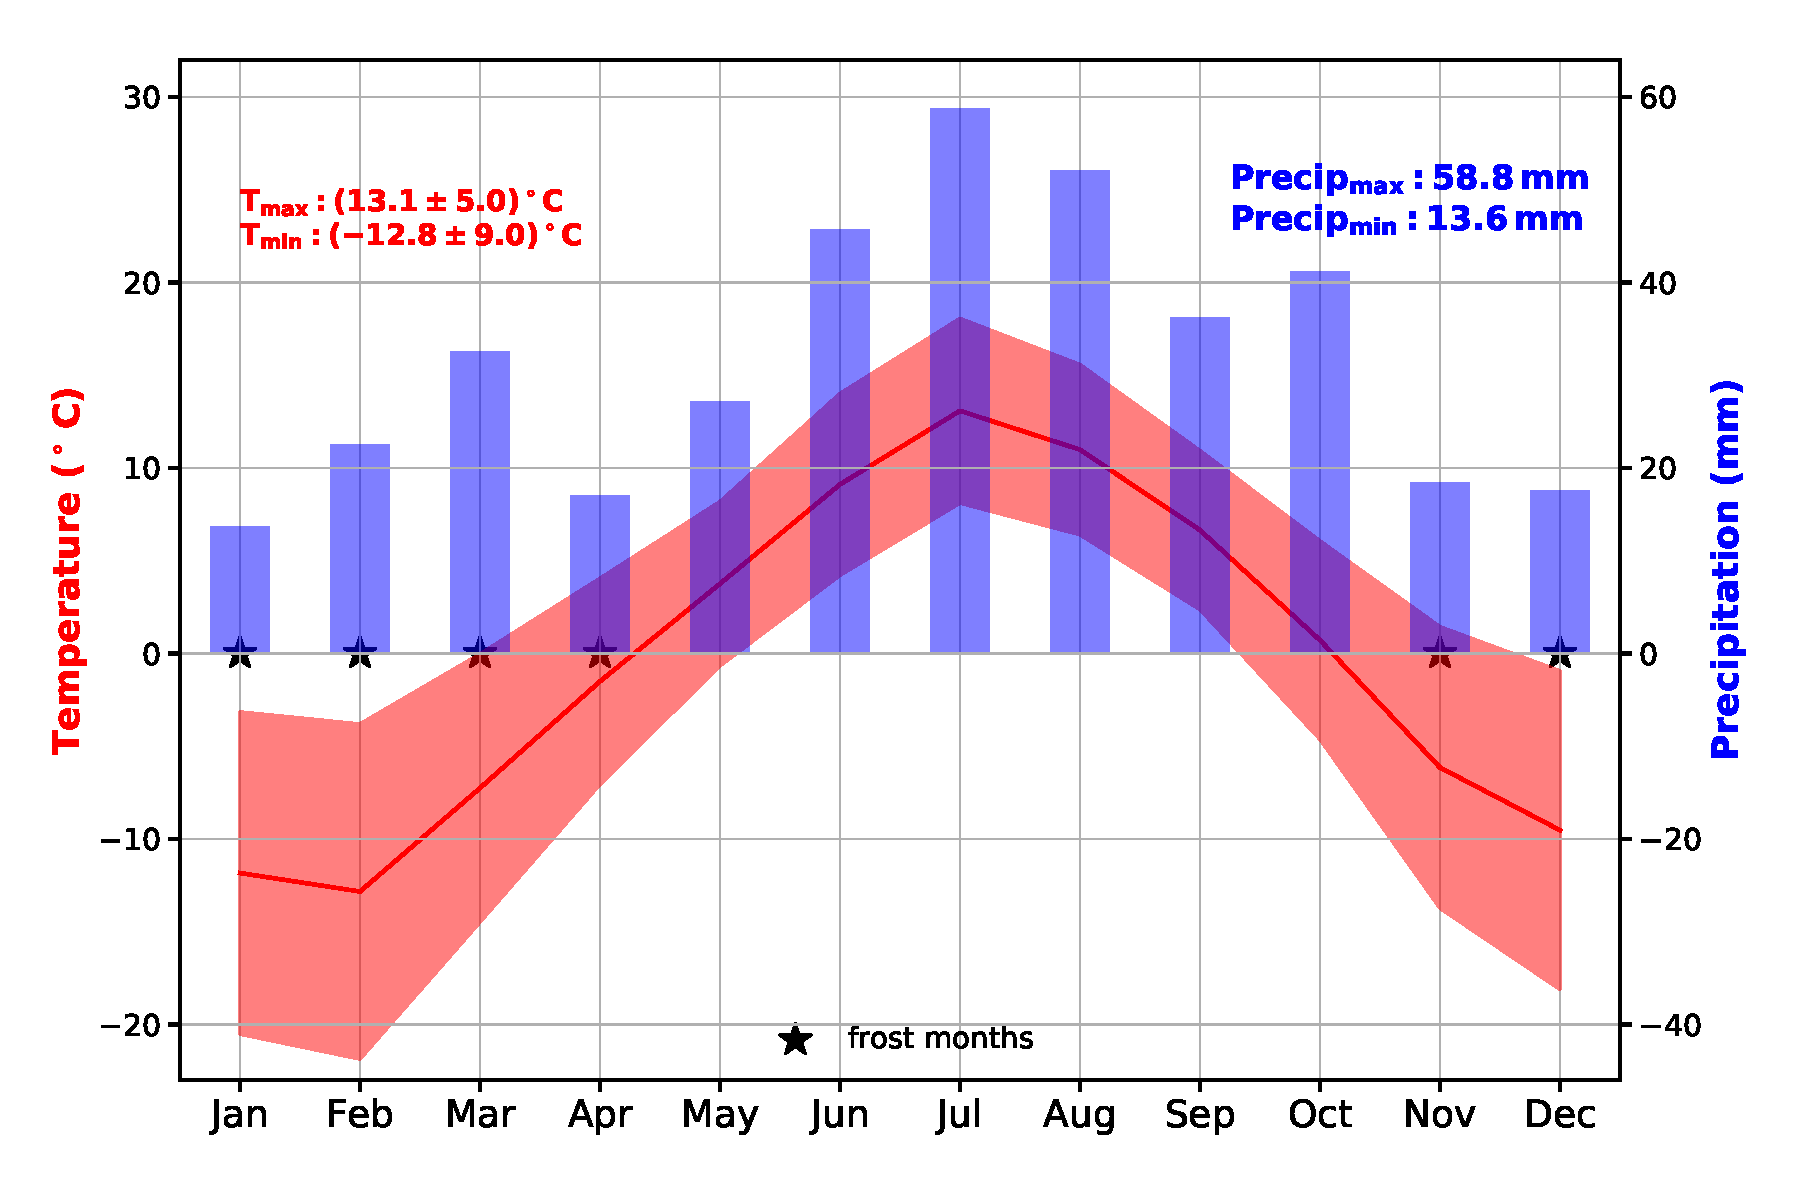
\includegraphics[width=8.3cm]{climatediagram}
  \caption{Climate diagram following Walter and Lieth. The diagram is based on climatological data for Svanvik/Pasvik (1992--2012) downloaded from LandbruksMeteorologiske Tjeneste. Monthly averaged temperatures (red line) are displayed with standard error of mean as error band. Averaged monthly accumulated precipitation (blue bars) is shown with standard deviation of mean as error bars. Months with average temperatures below freezing are denoted with a star.}
  \label{fig:climatediagram}
\end{figure}

\subsubsection{Ozone}
\label{subsubsec:clim_ozone}
In the following, we will look at derived ozone climatologies from different perspectives.
The multi-annual means of daily mean ozone, for simplicity here without standard deviations, at observation sites in northern Fennoscandia (refer to Table~\ref{tab:ebas_obs} for details) are shown in Fig.~\ref{fig:ozone_climatology_fenoscandic_obs}. All climatologies peak in spring, with peak values of about $48\,\unit{ppb}$ in late April. The annual average ozone concentration \chem{\left<[O_3]\right>} declines throughout the growing season until it reaches its minimum in late summer/fall ($24-30\,\unit{ppb}$). The turning points lie approximately in June and November. The ozone climatology lags about 3 months behind the temperature climatology. At Svanvik, \chem{\left<[O_3]\right>} is $6.6\,\unit{ppb}$ lower than on sites at Jergul/Karasjok (NOR), Esrange (SWE), and Pallas (FIN). The large spread in case of Svanvik and Janiskoski can be explained due to the lower overall statistics.

\begin{figure}[t]
  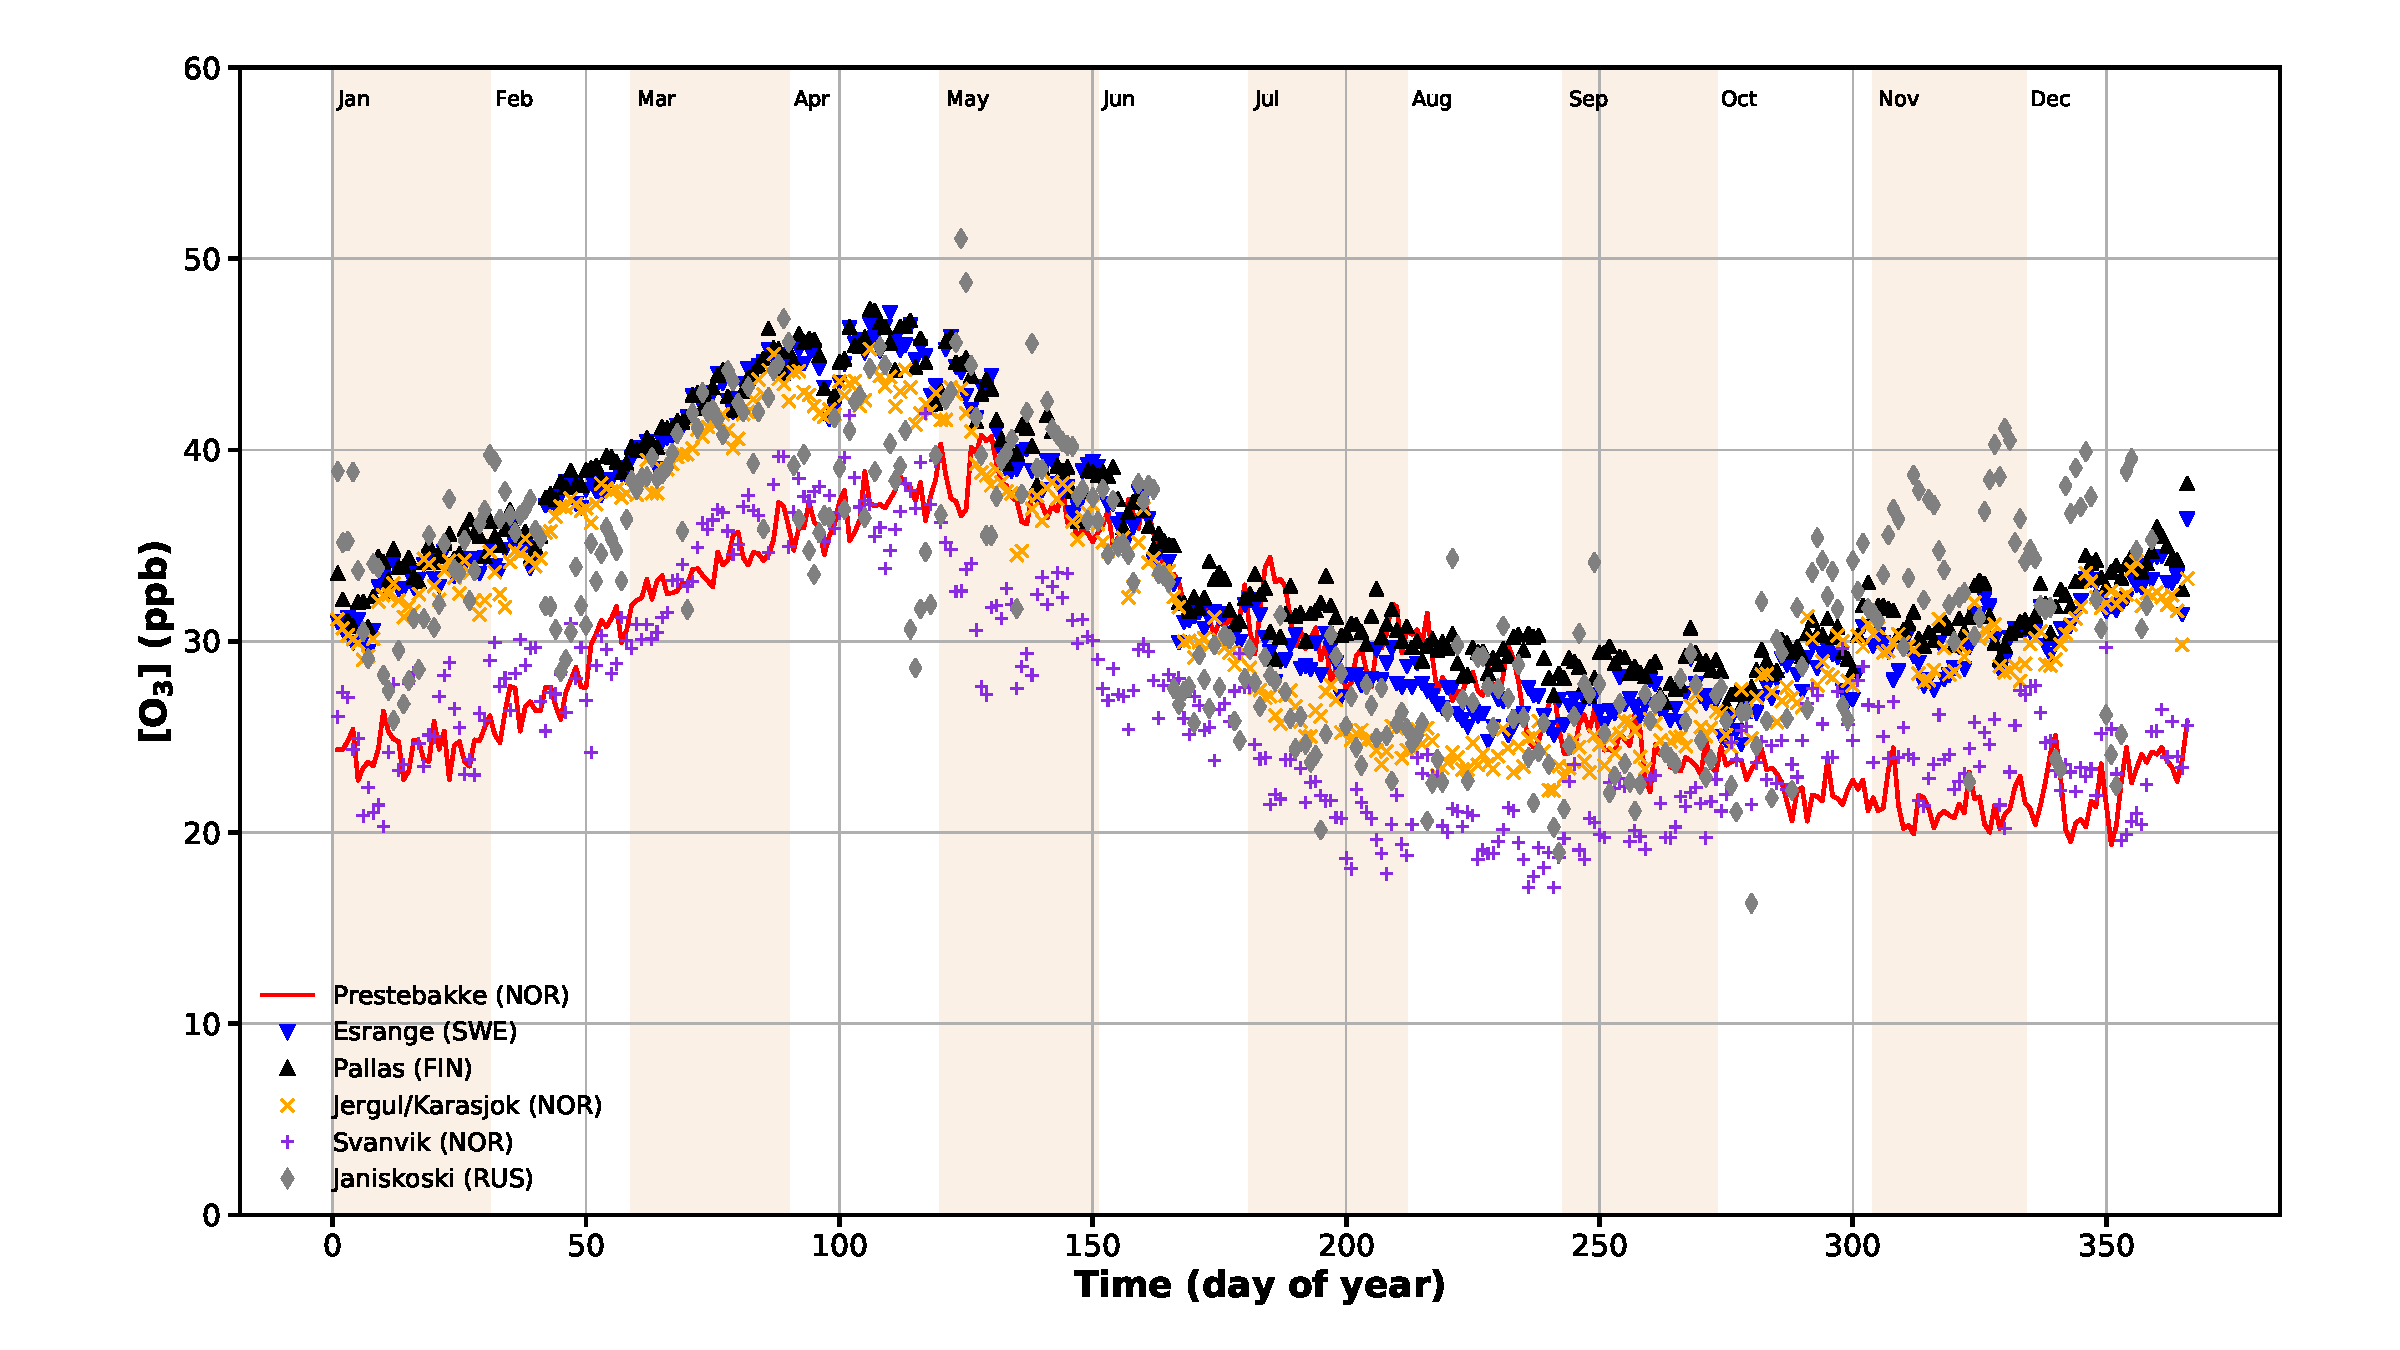
\includegraphics[width=8.3cm]{ozone_climatology_fenoscandic_obs}
  \caption{Multi-annual mean of daily mean ozone at observation sites in Fennoscandia. The large spread in case of Svanvik and Janiskoski is due to the lower statistics. All climatologies peak in spring, with peak values in April. The annual average ozone concentration \chem{\left<[O_3]\right>} at Svanvik is $6.6\,\unit{ppb}$ lower than at the sites at Jergul/Karasjok (NOR), Esrange (SWE), and Pallas (FIN).}
  \label{fig:ozone_climatology_fenoscandic_obs}
\end{figure}

The correlation of \chem{[O_3]} between Esrange, Pallas, and Jergul/Karasjok is fairly high ($r^2\approx 0.8$, Appendix Fig.~\ref{fig:density_distribution}a, b), hence we can put those data series together to derive a general ozone climatology for northern Fennoscandia. The correlation between Svanvik and Esrange and Pallas is rather low, 0.4 and 0.6, respectively. Thus, Svanvik cannot directly be represented by any measurements taken at either Esrange or Pallas. We shall come back to this in Section~\ref{subsec:ozone_reco}.

In Figure~\ref{fig:ozone_climatology_fenoscandic_obs_spline}, the 2 dimensional density distributions for the thus defined northern Fennoscandia (Fig.~\ref{fig:ozone_climatology_fenoscandic_obs_spline}a) and Svanvik (Fig.~\ref{fig:ozone_climatology_fenoscandic_obs_spline}b) are shown. Darker colors indicate higher probability to observe these values. On top of the density distributions, $10\,\unit{days}$ averages of daily mean \chem{\left<[O_3]\right>_\mathrm{10\,\unit{d}, mean}}, daily maximum \chem{\left<[O_3]\right>_\mathrm{10\,\unit{d}, max}}, and daily minimum \chem{\left<[O_3]\right>_\mathrm{10\,\unit{d}, min}} are displayed together with the $1 \sigma$ uncertainties, respectively. In addition, \chem{\left<[O_3]\right>_\mathrm{10\,\unit{d}, mean}} is also shown with standard error of mean (albeit small and hardly visible). Splines have been fitted through the data for easier inter-comparison with reanalysis data.

From the northern Fennoscandic climatology, one can deduce several features. The maximum of \chem{\left<[O_3]\right>_\mathrm{10\,\unit{d}, min}} peaks about $20\,\unit{days}$ earlier than the \chem{\left<[O_3]\right>_\mathrm{10\,\unit{d}, mean}}, and \chem{\left<[O_3]\right>_\mathrm{10\,\unit{d}, max}}. With respect to the periodicity of \chem{\left<[O_3]\right>_\mathrm{10\,\unit{d}, mean}}, it takes about $7.5\,\unit{months}$ from minimum concentration to maximum concentration, while from maximum to minimum it only takes about $4.5\,\unit{months}$. The maximum of \chem{\left<[O_3]\right>_\mathrm{10\,\unit{d}, max}} is at $52\,\unit{ppb}$ in late April and the minimum of \chem{\left<[O_3]\right>_\mathrm{10\,\unit{d}, min}} occurs at $15\,\unit{ppb}$ in the beginning of September. The steep rise of \chem{\left<[O_3]\right>_\mathrm{10\,\unit{d}, mean}} in spring is in coincidence with increasing temperatures as well as increase in global irradiance. The decrease in \chem{\left<[O_3]\right>_\mathrm{10\,\unit{d}, mean}} begins about one month ahead of the estimated onset of the greening season. Based on data from SeNorge.no and the agricultural rule of thumb that the daily average temperature has to be above $5\,\unit{^\circ C}$ for $5\,\unit{days}$ consecutively, we find $\left<G_\mathrm{begin}\right> = (150 \pm 14)\,\unit{days of the year}$ at Svanvik (Appendix Fig~\ref{fig:greening_season_change_Svanvik}), which translates into the end of May.

The density distribution for Svanvik and the respective \chem{\left<[O_3]\right>_\mathrm{10\,\unit{d}, mean}}, and \chem{\left<[O_3]\right>_\mathrm{10\,\unit{d}, max}} (Fig.~\ref{fig:ozone_climatology_fenoscandic_obs_spline}b) display a similar pattern as the northern Fennoscandic climatology. The spring peak apparently occurs slightly earlier (in the beginning of April). As Svanvik is located at lower altitude than the other sites, the earlier ozone peak may point to an interplay with ozone uptake by vegetation. {\bf TODO: The data from SeNorge seems to point to a later onset of greening, than what I interfered from OpenIFS data. This means that the beginning of the growing season is not a good measure for the termination of the ozone spring peak. This does not exclude the early start of pine forest photosynthesis as a driver. Coniferous forest starts to photosynthesis earlier than what the growing season begin would mark. \chem{CO_2} uptake and phenology of coniferous trees \citep{TB:Kolari2007} starts as early as doy 100, acclimates to leaf temperature history - photosynthesis drops at around doy 200--250.} The average ozone concentration at Svanvik is lower than at the other sites, as already mentioned, which is in league with a decrease in tropospheric ozone with decreasing altitude. In July--September, ozone is occasionally almost completely depleted during night time.

\begin{figure}[t]
  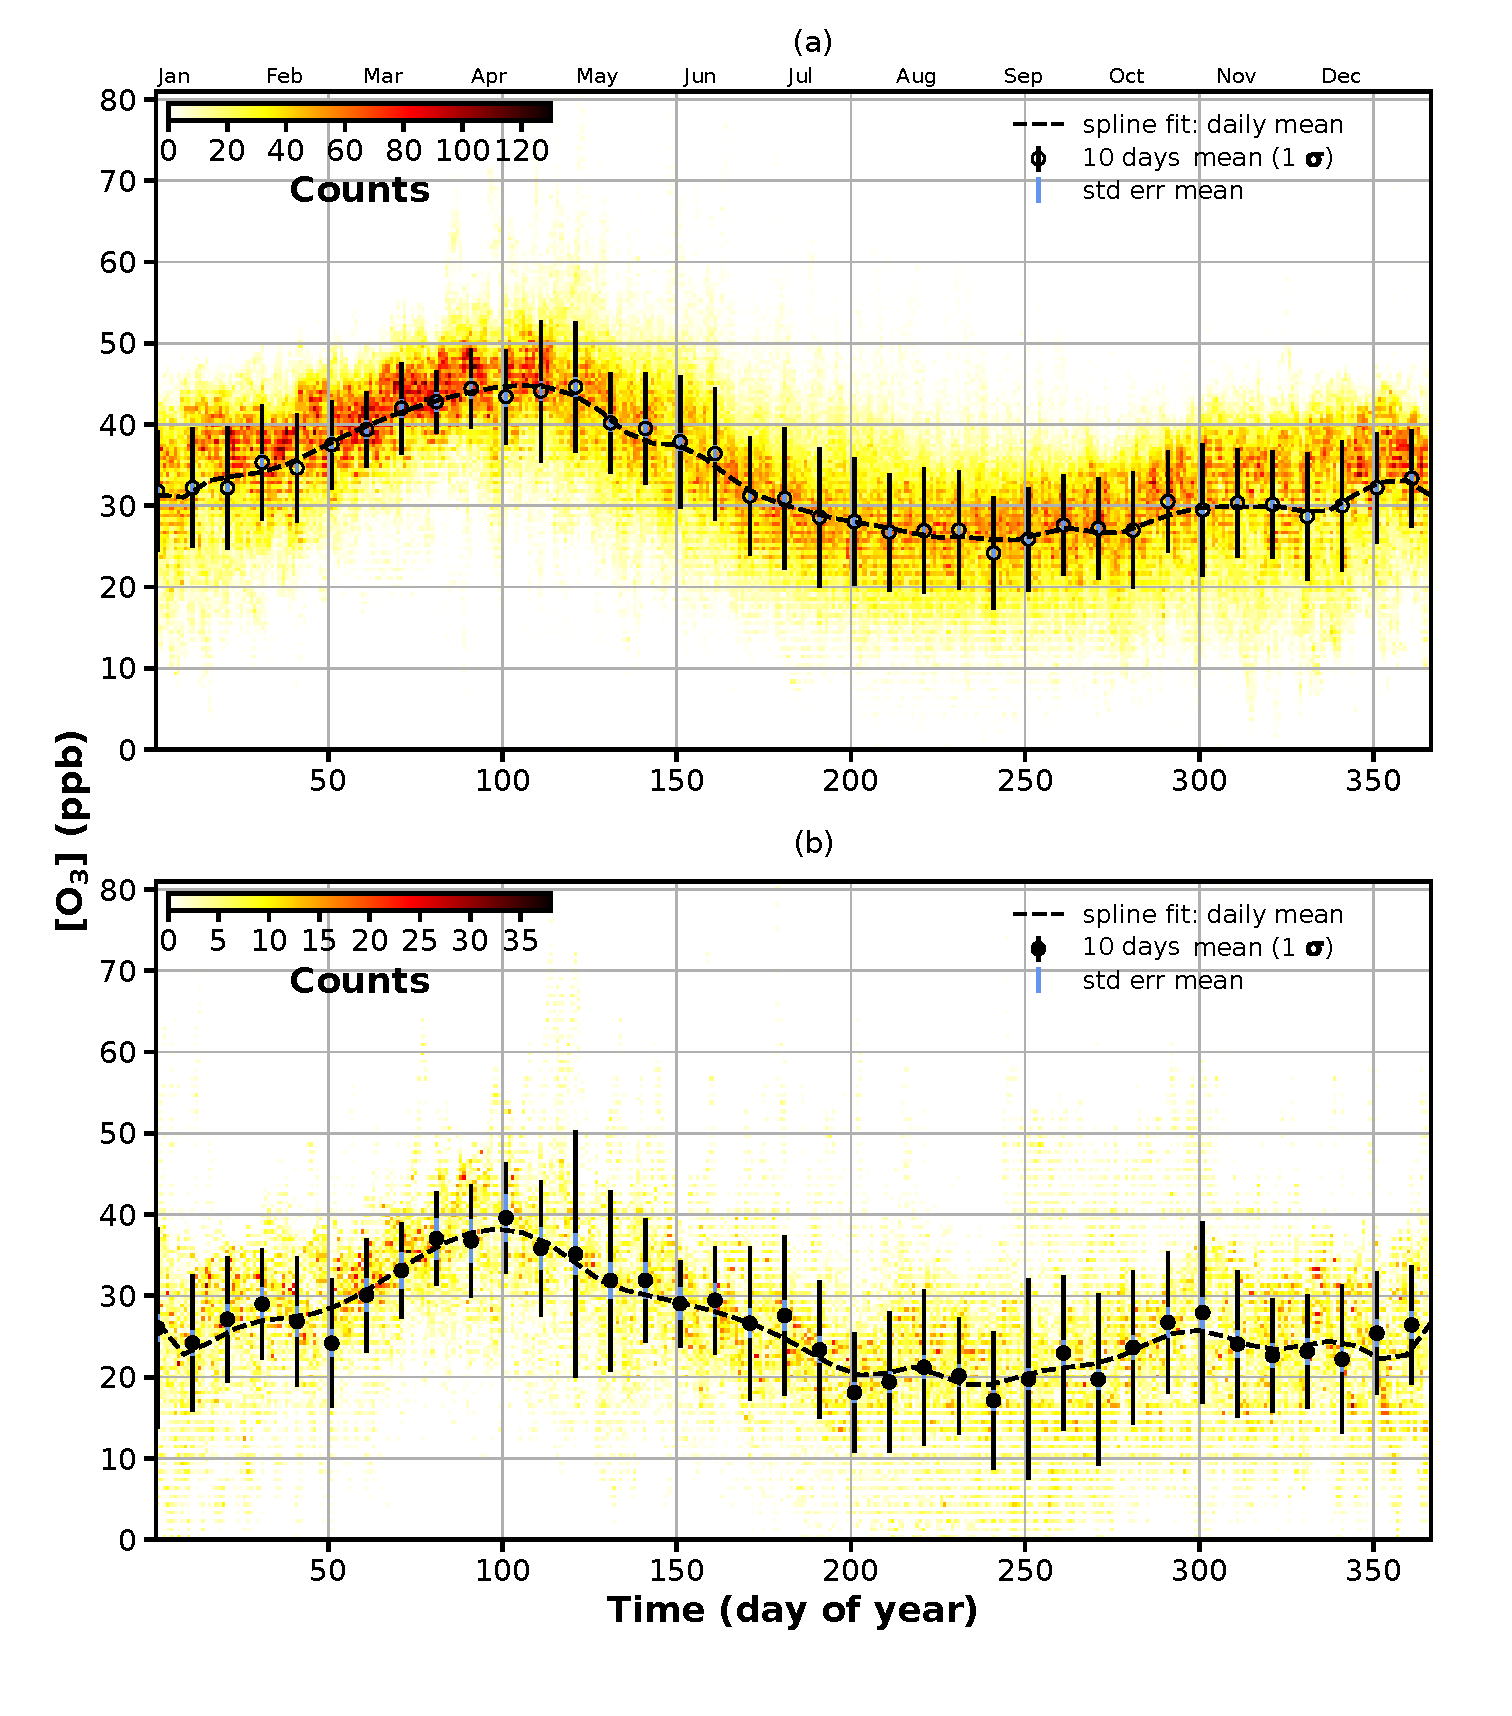
\includegraphics[width=8.3cm]{ozone_climatology_fenoscandic_obs_spline}
  \caption{Derivation of ozone climatologies. Density distributions are shown together with multi-annual mean of daily ozone concentrations \chem{[O_3]}. Splines have been fitted though daily mean and max \chem{[O_3]}. The climatology of daily mean ozone is shown together with $1\,\sigma$ standard deviation and standard error of the mean. Since \chem{[O_3]} are strongly correlated for sites at Jergul/Karasjok (NOR), Esrange (SWE), and Pallas (FIN) (see Fig.~\ref{fig:density_distribution}), data of these have been averaged together to derive a climatology for northern Fennoscandia. (a) Northern Fennoscandia; (b) Svanvik.}
  \label{fig:ozone_climatology_fenoscandic_obs_spline}
\end{figure}

Finally, we shall look at the comparison of climatologies derived from observational ozone data and the various reanalysis products (Fig.~\ref{fig:ozone_climatologies}). As representative for the sites, the nearest neighboring grid point has been chosen. The ECMWF products do not reproduce observed surface ozone well. The MACC reanalysis (Fig.~\ref{fig:ozone_climatologies}a) is in general too low ($(9\pm 7)\,\unit{ppb}$) and displays a erroneous seasonal cycle. Ozone concentrations peak already in March followed by a second peak in July. Also CAMSRA matches the observed ozone climatology poorly (Fig.~\ref{fig:ozone_climatologies}b). Despite displaying only one ozone peak, it still does not reproduce the seasonality in northern Fennoscandia well. The CAMSRA spring peak appears to lag behind by $1\,\unit{month}$ and is $5\,\unit{ppb}$ lower, whereas the minimum occurs in January compared to August/September. The annual amplitude ($(26\pm 1)\,\unit{ppb}$) is larger than in the climatology derived from observations ($19\,\unit{ppb}$). Modeled \chem{[O_3]} at Svanvik are even slightly higher than at Pallas. In contrast, the ensemble mean of the Copernicus regional model reanalysis does reproduce the seasonal cycle in northern Fennoscandia quite well (Fig.~\ref{fig:ozone_climatologies}c), but is on average still slightly too low ($(2.8\pm 0.5)\,\unit{ppb}$).

\begin{figure}[t]
  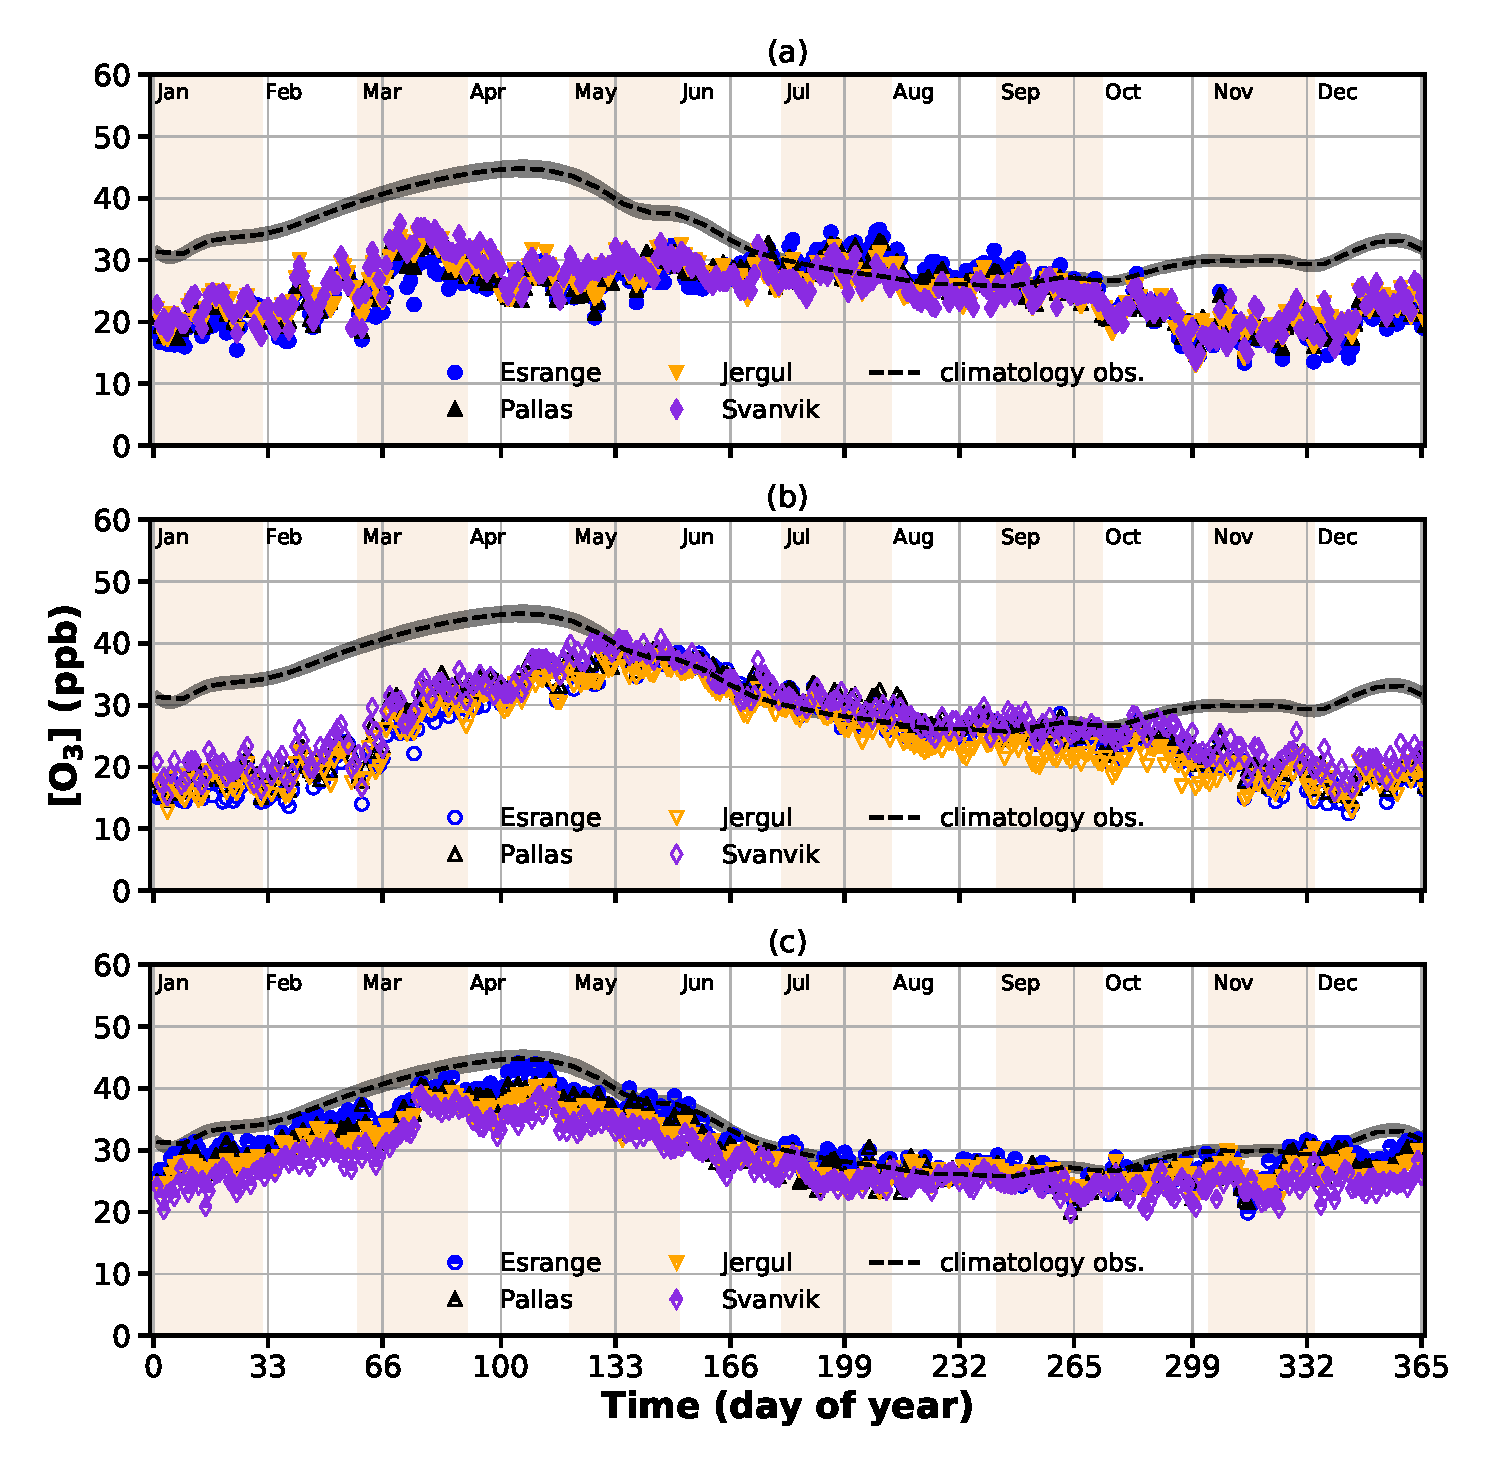
\includegraphics[width=8.3cm]{ozone_climatologies_portrait}
  \caption{Comparison of climatologies derived from observational data (EBAS, see Fig.~\ref{fig:ozone_climatology_fenoscandic_obs}) with various ozone reanalysis products: (a) ECMWF: MACC reanalysis; (b) ECMWF: CAMS reanalysis; (c) Copernicus: Regional model reanalysis ensemble mean. As representative for the sites, the nearest neighboring grid point has been chosen. The ECMWF products do not reproduce observed surface ozone well. The MACC reanalysis is in general too low and displays a erroneous seasonal cycle. The CAMS reanalysis matches better but does not reproduce the seasonality in northern Fennoscandia. The ensemble mean of the Copernicus regional model reanalysis does reproduce the seasonal cycle in northern Fennoscandia, though the modeled ozone concentrations are slightly too low.}
  \label{fig:ozone_climatologies}
\end{figure}

There are many probable explanations for the discovered differences in the climatologies derived from the three reanalyses. The effective changes from the MACC reanalysis to CAMSRA have been reported and discussed by \citet{ACP:Inness2019} on a global level. Amongst others, an assimilation of ozone profiles from satellite retrieval and an upgraded ozone chemistry scheme have lead to the enhanced performance of latter. The higher spatial resolution of the regional air quality models used in the CAMS Regional Ensemble compared to the global reanalyses does capture more localized depletion and peak episodes in \chem{[O_3]} better and enhances the capability of the models with respect to daily and seasonal cycles in ozone {\bf TODO: Any citable source for this assumption?}. Latter is, of course, also affected by upgrades in the OpenIFS used as meteorological forcing. However, we can assume that the main driver for the strikingly different results are the assimilated observational ozone data. Satellite retrievals resolve \chem{[O_3]} at the surface rather poorly and hence do not constrain the global models well enough {\bf TODO: Any citable source for this?}.

\subsection{2018/19 anomalies}
\label{subsec:anomalies}
Using these established climatologies, we look at the anomalies in 2018/19 and discuss the differences between the two years. 

\subsubsection{Temperature, precipitation, and global irradiance}
\label{subsubsec:anomal_tpq}
In Fig.~\ref{fig:plot_temperature_anomalies_svanvik}, temperature anomalies at Svanvik are shown as percentage of days warmer/colder than $\pm 1\,\sigma$ from the climatological mean for each month. Negative deviations from climatology are displayed as negative percentage. The full annual positive/negative deviations are indicated in the respective corners (right upper/right lower). The hatched area between the dashed lines indicates the expected percentage of values falling above/below $\pm 1\,\sigma$ if a normal distribution is assumed ($15.9\,\unit{\%}$). The summer of 2018 was significantly warmer than average. Especially in May and July more than $40\,\unit{\%}$ of days were significantly warmer than normal temperature. Temperatures continued to be significantly warmer throughout fall into early winter (August--November) with the exception of October. March 2018 was unusually cold. The summer of 2019 was fairly average, however significantly colder in July, while August was both significantly colder and warmer. Temperatures in April were significantly warmer than average.

\begin{figure}[t]
  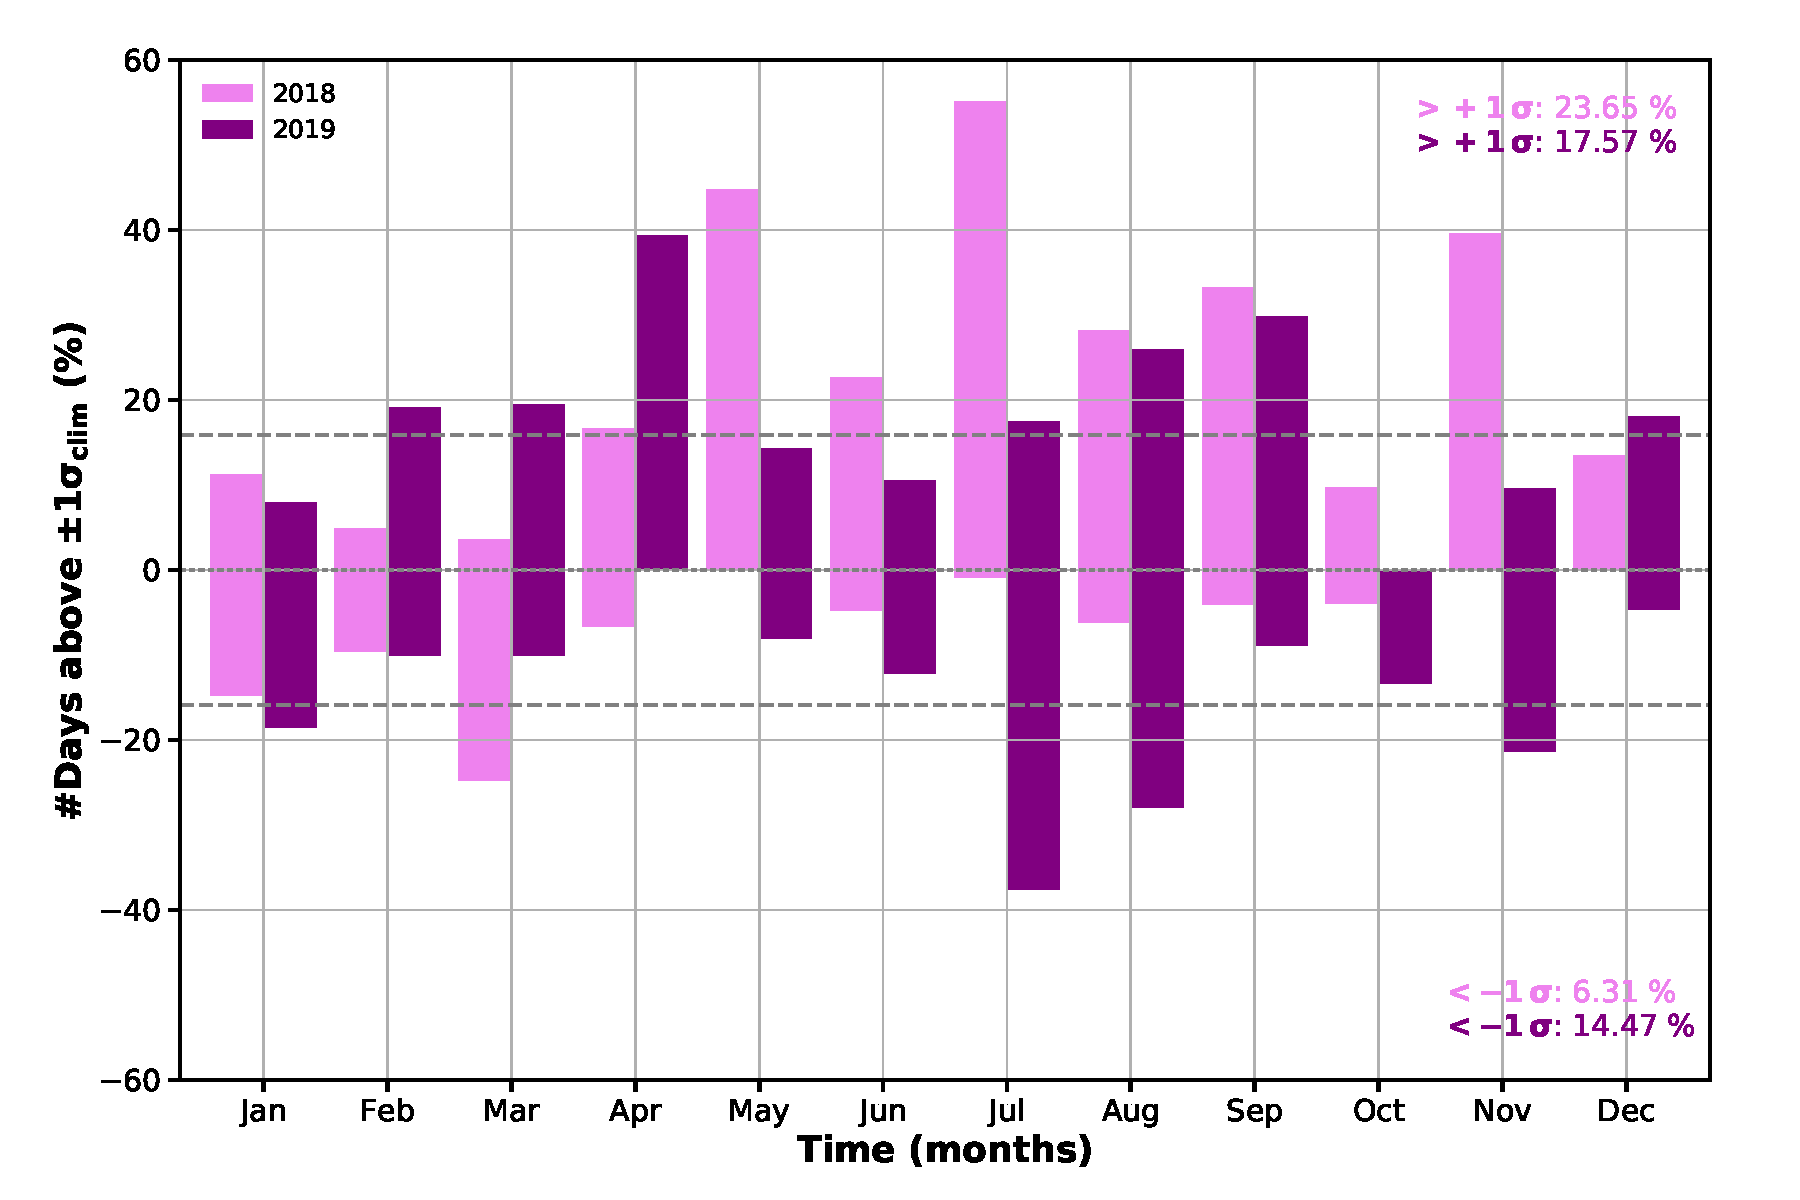
\includegraphics[width=8.3cm]{temperature_signific_1}
  \caption{Temperature anomalies at Svanvik. Percentage of days warmer/colder than $\pm 1\,\sigma$ from climatological mean displayed for each month. Negative deviations from climatology are shown as negative percentage. The annual positive/negative deviations are indicated in the respective corners (right upper/right lower). The hatched area between the dashed lines indicates the expected percentage of values falling above/below $\pm 1\,\sigma$ if a normal distribution is assumed ($15.9\,\unit{\%}$). The summer of 2018 was significantly warmer than average, especially May and July. The summer of 2019 was fairly average but significantly warmer than average in April and colder in July/August.}
  \label{fig:plot_temperature_anomalies_svanvik}
\end{figure}

In a similar way, the precipitation anomalies at Svanvik are displayed in Fig.~\ref{fig:plot_precipitation_anomalies_svanvik}. However, the percentage of days wetter/drier than $\pm \frac{1}{2}\,\sigma$ from the climatological mean is shown for each month, due to the larger variability in observed precipitation too few days showed a significance of $1 \sigma$ or higher. As above, negative deviations from the climatology are shown as negative percentage and annual positive/negative deviations are indicated in the respective corners. The hatched area between the dashed lines indicates the expected percentage of values falling above $\pm\frac{1}{2}\,\sigma$ if a normal distribution is assumed ($30.8\,\unit{\%}$). Unlike for the temperature anomalies, the picture is not as clear. While March 2018 was unusually wet, summer and fall (May/July, September/October) were significantly drier than average. 2019 was rather average throughout the year, with drier than usual fall (September/October) and a wet December.

\begin{figure}[t]
  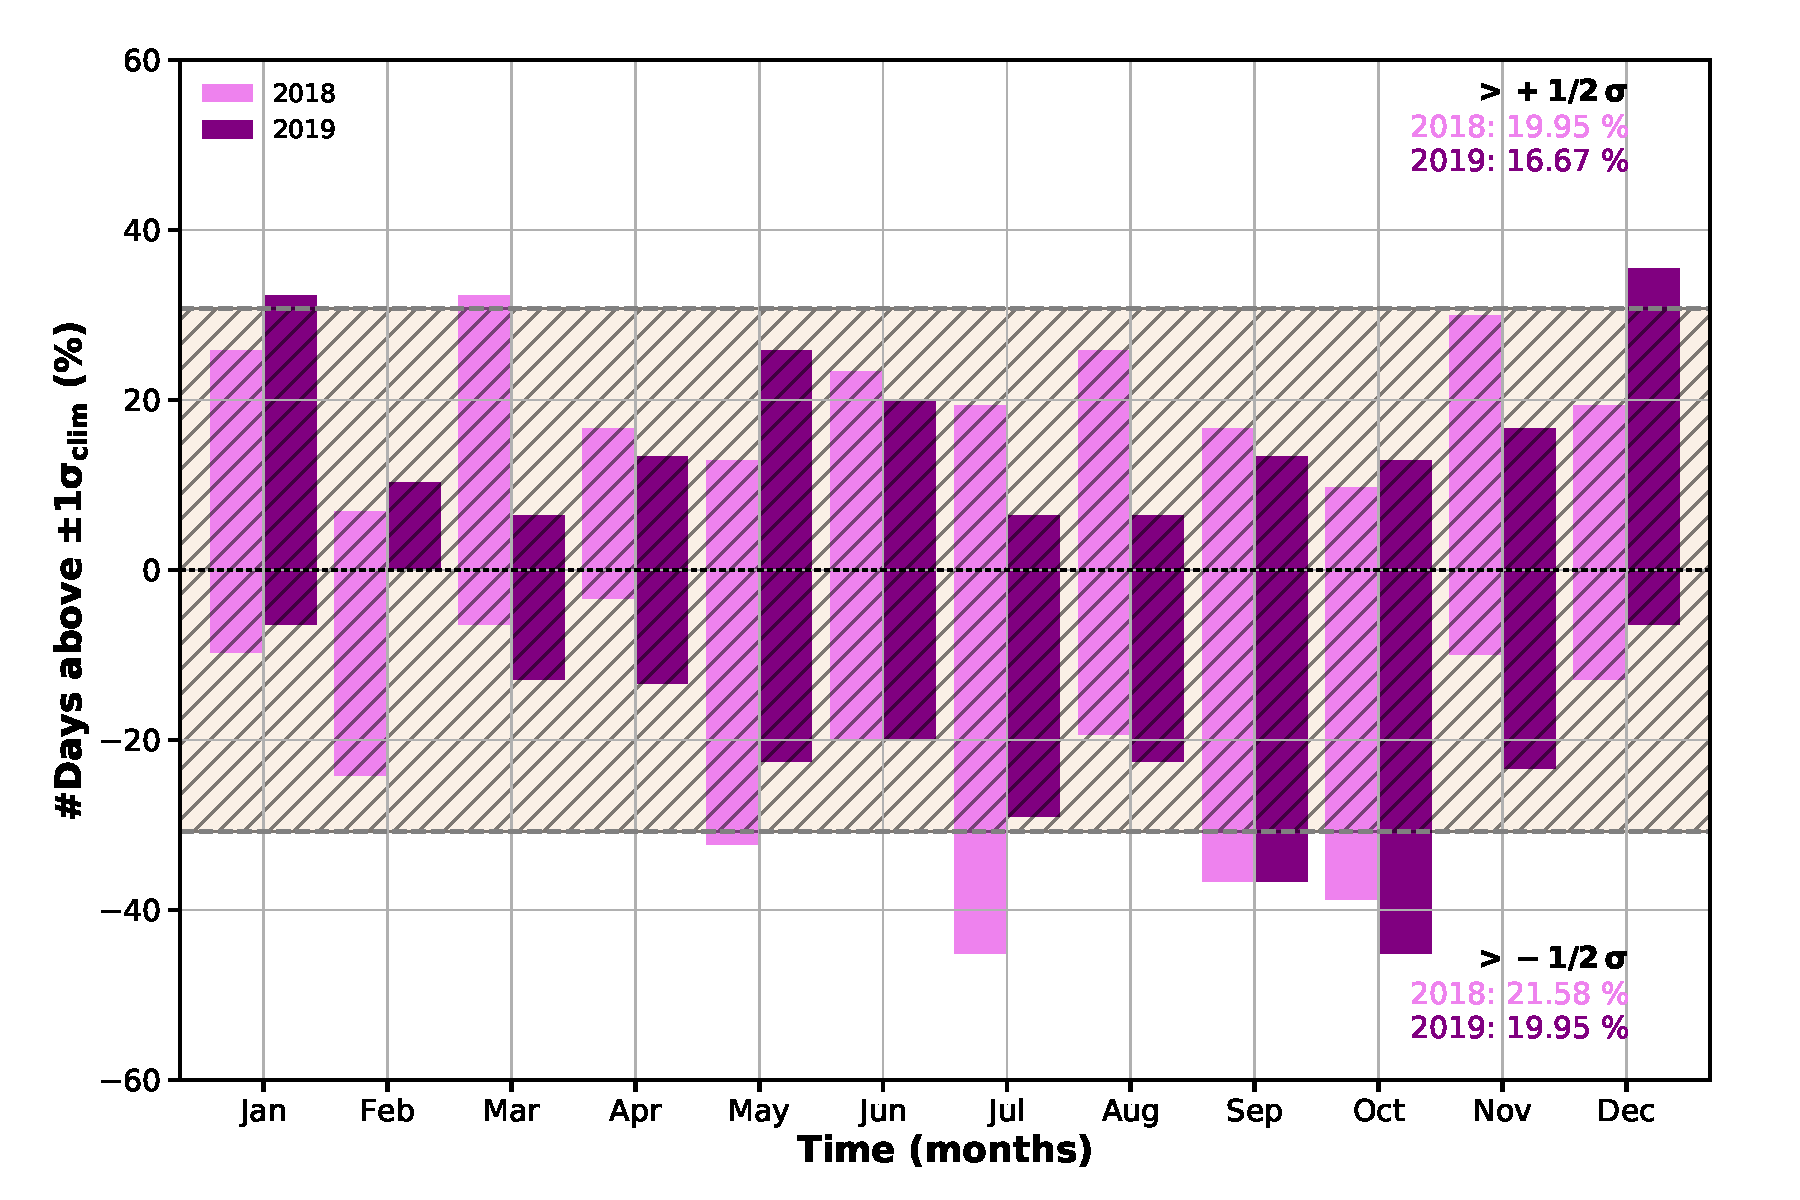
\includegraphics[width=8.3cm]{precipitation_signific_1}
  \caption{Precipitation anomalies at Svanvik. Percentage of days wetter/drier than $\pm \frac{1}{2}\,\sigma$ from climatological mean displayed for each month. Negative deviations from climatology are shown as negative percentage. The annual positive/negative deviations are indicated in the respective corners (right upper/right lower). The hatched area between the dashed lines indicates the expected percentage of values falling above $\pm\frac{1}{2}\,\sigma$ if a normal distribution is assumed ($30.8\,\unit{\%}$). Summer was significantly dry only in 2018, while fall was significantly dry in both years.}
  \label{fig:plot_precipitation_anomalies_svanvik}
\end{figure}

Similarly, the global irradiance anomalies at Svanvik are presented in Fig.~\ref{fig:global_rad_signific}. The percentage of days above/below $\pm 1\,\sigma$ from the climatological mean is displayed for each month. The hatched area between the dashed lines indicates the expected percentage of values falling above/below $\pm 1\,\sigma$ if a normal distribution is assumed. In summer 2018 (May/July), global irradiance was significantly higher than on average, while 2019 was generally an average year with a slightly darker spring (April/May).

\begin{figure}[t]
  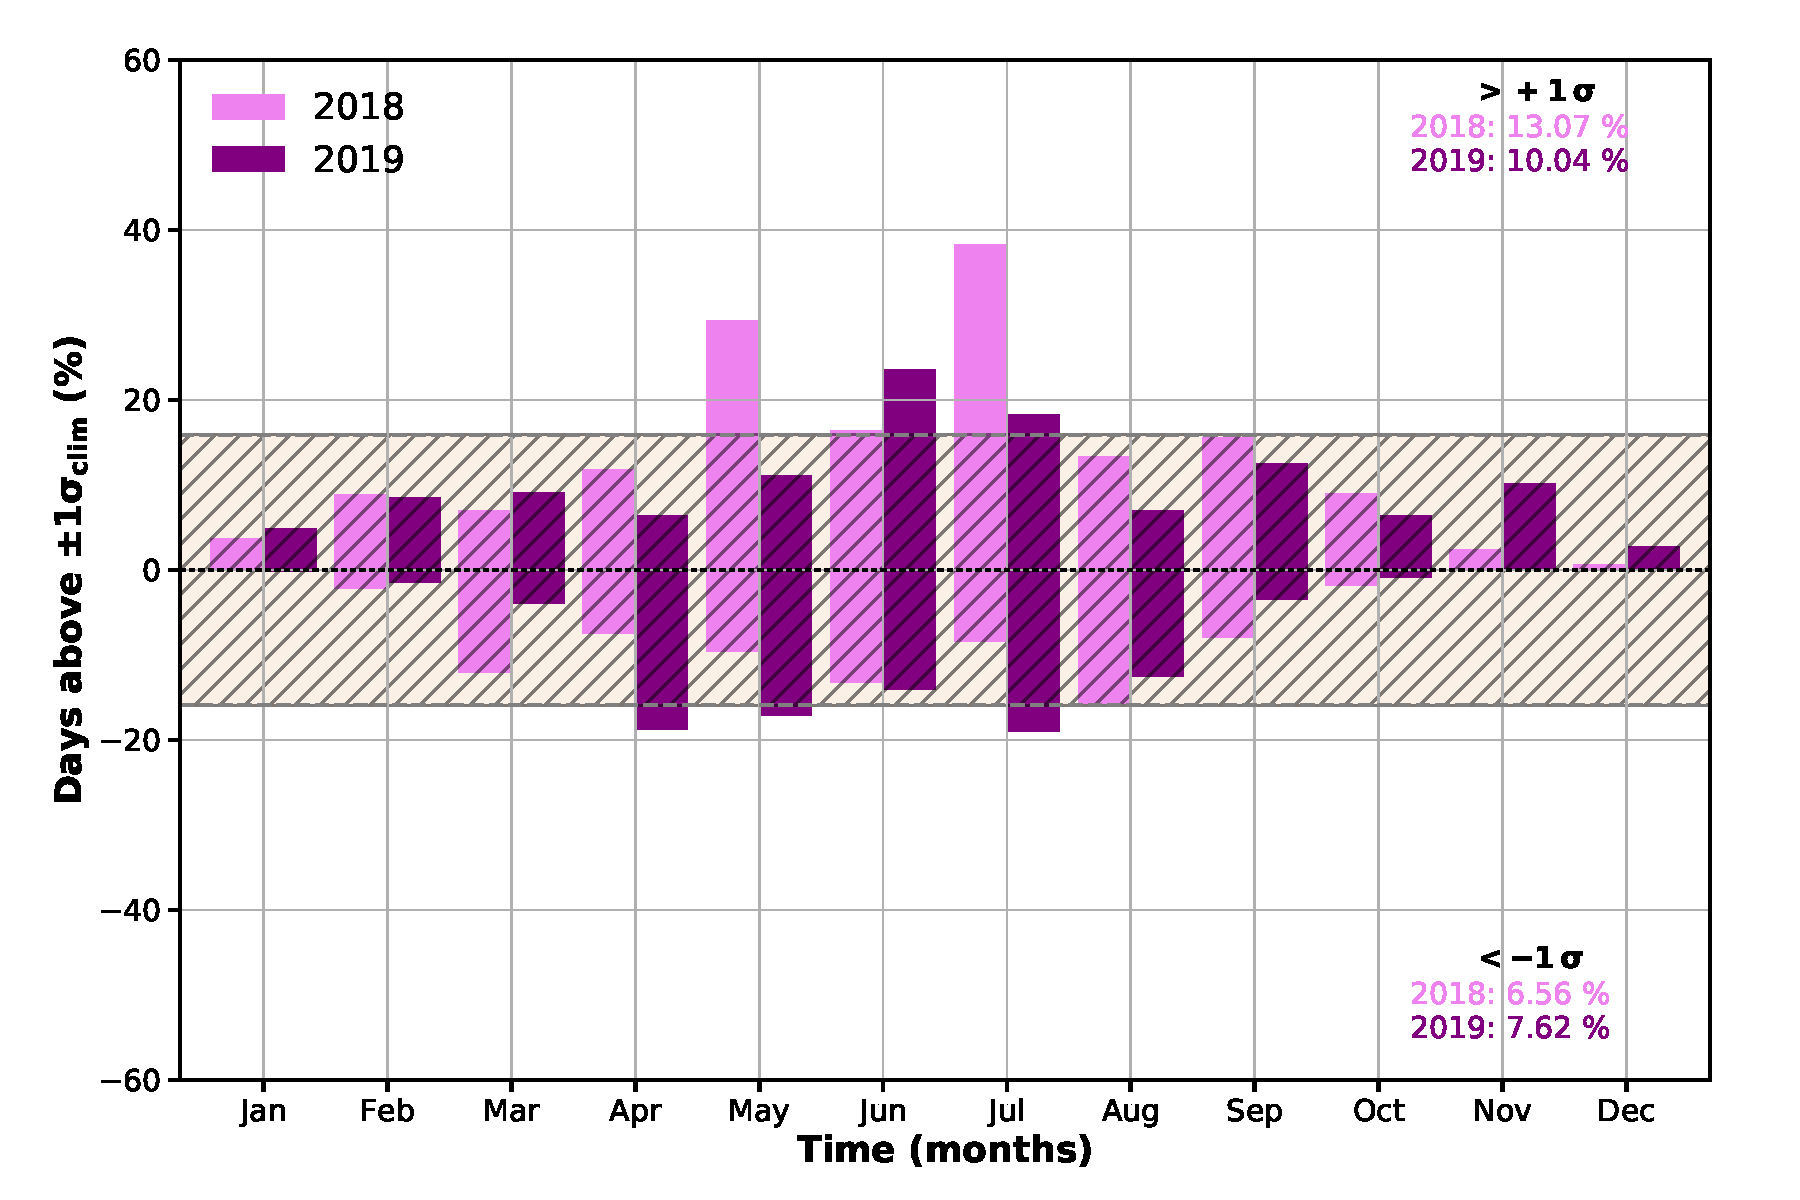
\includegraphics[width=8.3cm]{global_rad_signific_1}
  \caption{Global irradiance anomalies at Svanvik. Percentage of days above/below $\pm 1\,\sigma$ from climatological mean displayed for each month. Negative deviations from climatology are shown as negative percentage. The annual positive/negative deviations are indicated in the respective corners (right upper/right lower). The hatched area between the dashed lines indicates the expected percentage of values falling above/below $\pm 1\,\sigma$ if a normal distribution is assumed ($15.9\,\unit{\%}$). In summer 2018 (May/July), global irradiance was significantly higher than on average, while 2019 had significantly less than normal irradiance in April/May and more in June.}
  \label{fig:global_rad_signific}
\end{figure}

In summary, 2018 was significantly warmer, drier, and lighter than the climatological average, while 2019 was a rather average year.

\subsubsection{Ozone}
\label{subsubsec:anomal_ozone}
As we discussed in the preceding Section~\ref{subsubsec:anomal_tpq}, meteorological conditions in 2018 were significantly different from the climatological average. How does this translate into observed ozone anomalies \chem{\Delta[O_3]}?

If the data collected at Svanvik had been complete in 2018 and the climatology had extended into the resent past, we could have assessed the significance of ozone anomalies in the same way as for temperature, precipitation, and global irradiance. In Section~\ref{subsubsec:clim_ozone}, we described the construction of climatologies for northern Fennoscandia based on long term observations at Esrange, Jergul/Karasjok, and Pallas. For Svanvik this assessment is based on rather uncertain observations from 1986--1996. We also discussed the general patterns, similarities and differences. We shall now investigate \chem{\Delta[O_3]} in 2018/19 with respect to these climatologies in more detail.

In the following, we will use the interchangeable terms anomalies and residuals to distinguish between a climatological (anomalies) and a statistical (residuals) point of view.
All the above factors make it necessary to look not only at anomalies but statistically assess ozone concentration residuals at Svanvik as well as at Esrange and Pallas in comparison. Since the climatology of latter is more reliable, we will start with surface ozone concentration residuals \chem{\Delta[O_3]} at Esrange and Pallas in 2018. As data for 2019 has not yet been available from EBAS (last access, February 2020), we refrain from looking into these.

In Appendix Fig.~\ref{fig:ozone_climatology_fenoscandic_obs_residuals}, the probability density functions of daily mean ozone concentration residuals for Esrange and Pallas are shown. Both stations display a clear deviation from the climatological mean, however, not significant. On average, \chem{[O_3]} had been elevated by $(1.9\pm 5.7)\,\unit{ppb}$ and $(1.9\pm 5.4)\,\unit{ppb}$, respectively. Both distributions are slightly skewed towards positive deviations with $\frac{1}{4}$ of days (3. quantile, q3) falling above $5.8\,\unit{ppb}$ and $5.6\,\unit{ppb}$, respectively.

Appendix Figure~\ref{fig:ozone_climatology_fenoscandic_obs_residuals-Svanvik} displays the probability density functions of daily mean ozone concentration residuals for Svanvik based on data taken in 2018/19 with respect to the climatology derived for northern Fennoscandia (denoted NF in Appendix Fig.~\ref{fig:ozone_climatology_fenoscandic_obs_residuals-Svanvik}a) and the climatology derived for Svanvik (Appendix Fig.~\ref{fig:ozone_climatology_fenoscandic_obs_residuals-Svanvik}b).
As previously mentioned, \chem{\left<[O_3]\right>} at Svanvik are $(6.6\pm 7.1)\,\unit{ppb}$ lower than the northern Fennoscandic climatology. For 2018 and 2019, we find $\Delta\chem{\left<[O_3]\right>} = (-3.8\pm 5.6)\,\unit{ppb}$ and $\Delta\chem{\left<[O_3]\right>} = (-5.2\pm 5.0)\,\unit{ppb}$, respectively. While the probability density of the residuals between the two climatologies is skewed towards negative values, the skew of 2018/19 is positive.
With respect to the climatology for Svanvik (Appendix Fig.~\ref{fig:ozone_climatology_fenoscandic_obs_residuals-Svanvik}b), the probability density functions average for 2018/19 lies at $\Delta\chem{\left<[O_3]\right>} = (2.6\pm 5.8)\,\unit{ppb}$ and $\Delta\chem{\left<[O_3]\right>} = (1.2\pm 5.0)\,\unit{ppb}$, respectively.
Neither of the \chem{\Delta\left<[O_3]\right>} is significant by statistical means, but daily average ozone concentrations are slightly elevated in 2018 compared to 2019.

The \chem{\left<\Delta\left<[O_3]\right>\right>} for Svanvik in 2018 is slightly larger than for Esrange and Pallas. This could mean either that 2018 had been more exceptional at Svanvik or the derived climatology may need a correction for increased tropospheric background ozone concentration. Based on the meteorological conditions, we assume 2019 as average year which leads to a constant bias of about $1.2\,\unit{ppb}$. Daily \chem{\Delta_{present-past}\left<[O_3]\right>} from Esrange and Pallas, wherein present is defined as the average of 2010--2018 and past as the respective beginning of data taking until 1997, do not reveal a clear trend: We find for Esrange $(1.5\pm 3.1)\,\unit{ppb}$ and for Pallas $(-2.5\pm 3.7)\,\unit{ppb}$. Former is compatible with our assumed bias for the climatology derived for Svanvik.

To further investigate the ozone residuals, we conduct a Student's~t-test ($t = \frac{\chem{\Delta[O_3]}}{\sigma}$), assuming the same sample uncertainty $\sigma$ in both, climatology and the year in question. Results for Esrange and Pallas are shown in Appendix Fig.~\ref{fig:ozone_climatology_fenoscandic_obs_test}. This t-test clearly shows, that at both sites the residuals are significant on the $1\sigma$ level for at least $50\,\unit{\%}$. In Appendix Fig.~\ref{fig:ozone_climatology_fenoscandic_obs_test-Svanvik}, the test statistics for Svanvik are displayed. From Appendix Fig.~\ref{fig:ozone_climatology_fenoscandic_obs_test-Svanvik}a), we can deduce, that the residuals between the Svanvik climatology and the northern Fennoscandic climatology are significant on the $2\sigma$ level for at least half of the data, while the residuals are less certain in 2018 and 2019. In Appendix Fig.~\ref{fig:ozone_climatology_fenoscandic_obs_test-Svanvik}b) the same is shown for the years 2018/19 with respect to the climatology from Svanvik. We find that less than $50\,\unit{\%}$ of ozone concentration residuals are significant on the $1\sigma$ level.

In accordance to the above findings, we adjust the derived ozone climatology for Svanvik by adding a constant bias correction factor $\Delta\chem{[O_3]_\mathrm{bias-corr}} = 1.2\,\unit{ppb}$ and estimate the ozone concentration anomalies for 2018/19. In Fig.~\ref{fig:ozone_signific}, the resulting percentage of days above/below $\pm 1\,\sigma$ from the bias-corrected climatological mean is displayed for each month. Negative deviations from climatology are shown as negative percentage. Note that missing bars for certain months are both due to data availability (see Section~\ref{subsubsec:atmo_svanvik} for details about the time range of data taking at Svanhovd) and anomalies not meeting the criteria of $\pm 1\sigma$ deviation from climatological mean. In April/May 2018, ozone was significantly enhanced, while 2019 was generally an average year. In both years, ozone concentrations were significantly below average in November. July 2018 has not been corrected for the missing data due to data acquisition problems. The corrected value is, however, indicated by the star (refer to Section~\ref{subsec:ozone_reco} for details of the used method for gap filling).

\begin{figure}[t]
  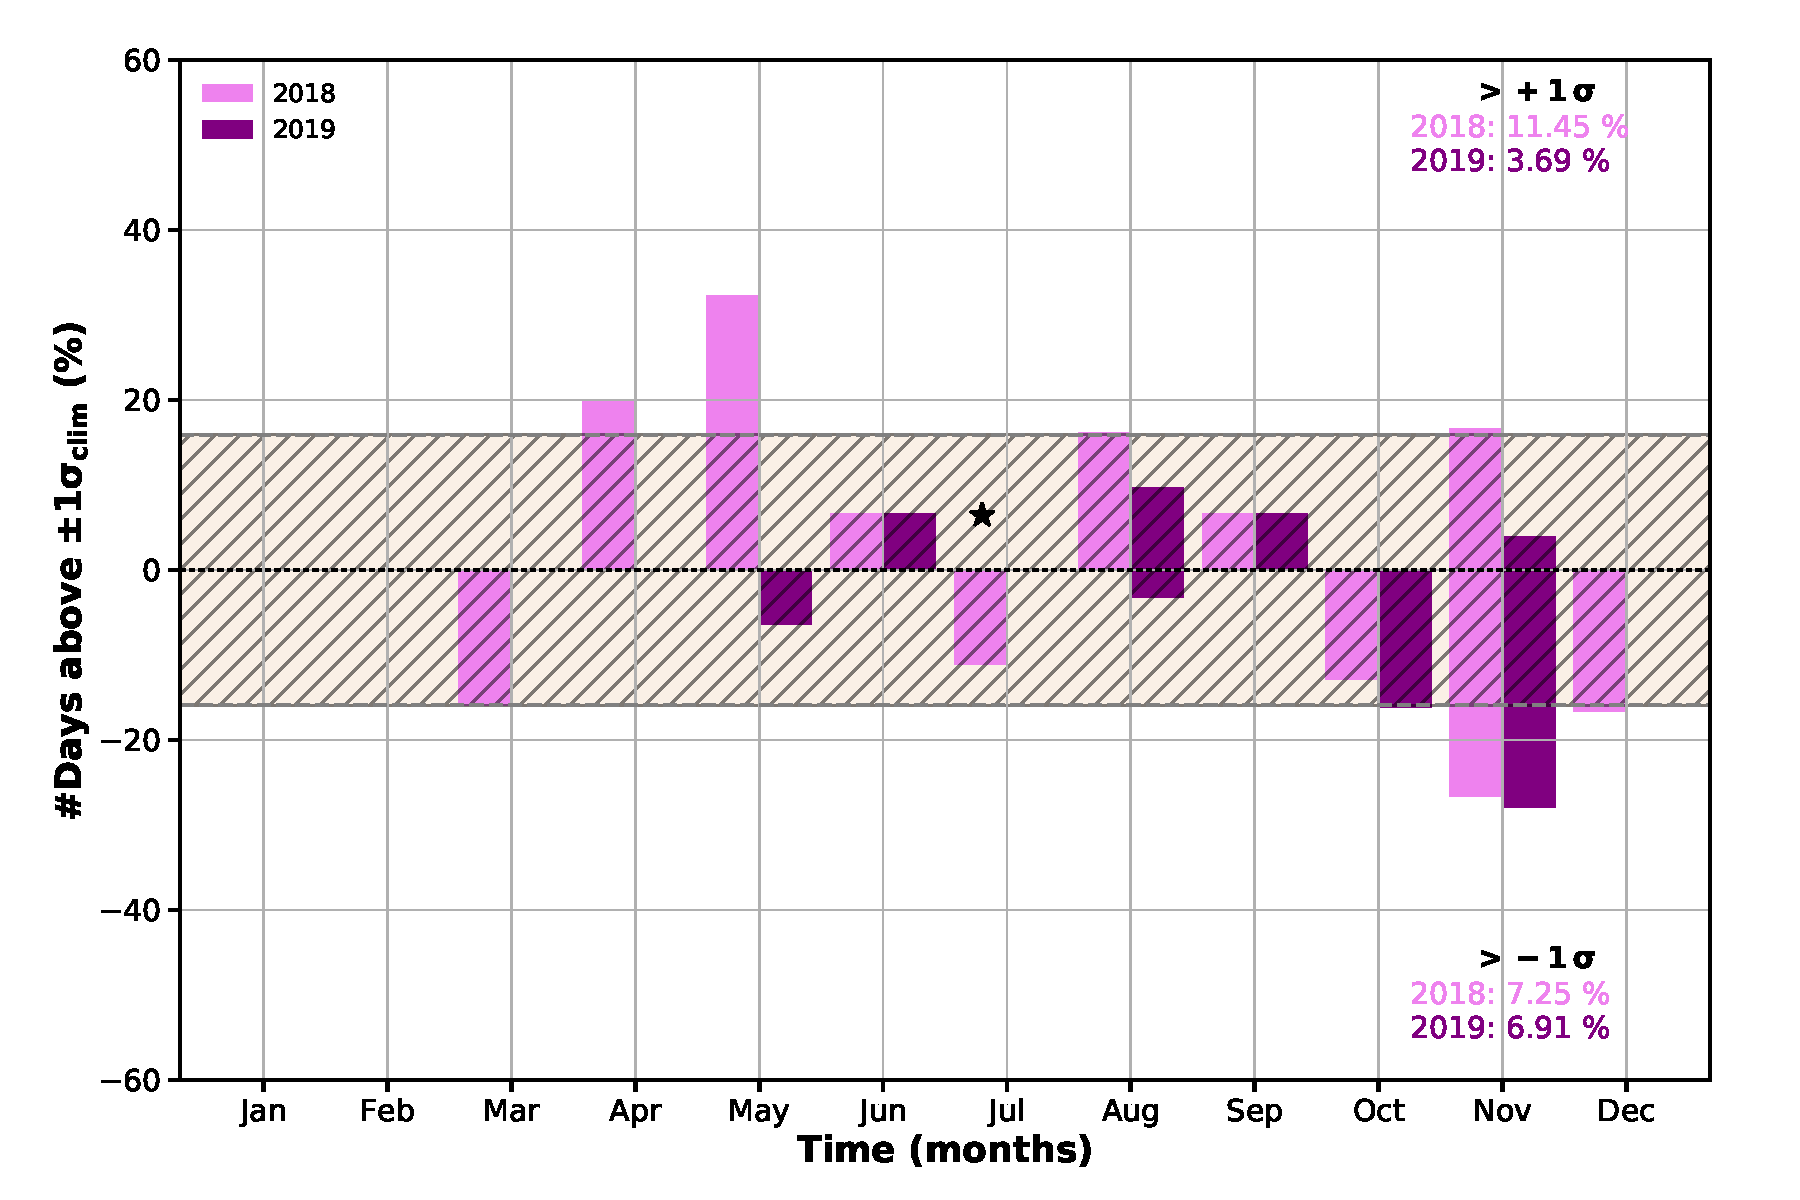
\includegraphics[width=8.3cm]{ozone_signific_1}
  \caption{Ozone concentration anomalies at Svanvik. Ozone climatology has been corrected for an constant negative bias of $-1.2\,\unit{ppb}$. Percentage of days above/below $\pm 1\,\sigma$ from climatological mean displayed for each month. Negative deviations from climatology are shown as negative percentage. The annual positive/negative deviations are indicated in the respective corners (right upper/right lower). The hatched area between the dashed lines indicates the expected percentage of values falling above/below $\pm 1\,\sigma$ if a normal distribution is assumed ($15.9\,\unit{\%}$). July 2018 has not been corrected for the missing data due to data acquisition problems. The corrected value is indicated by the star (refer to Section~\ref{subsec:ozone_reco} for details). In April/May 2018, ozone was significantly higher than on average, while 2019 was generally an average year. In both years ozone concentrations were significantly below average in November.}
  \label{fig:ozone_signific}
\end{figure}

To conclude, ozone concentrations in 2018 have been elevated compared to the respective climatologies, however, on average not significantly by statistical means. At Esrange and Pallas at least $25\,\unit{\%}$ (3.~quantile) of anomalies are significant on a $3\sigma$ level or more, while at Svanvik the 3.~quantile lies at about $2\sigma$. This means that in 2018 the stations at Esrange and Pallas saw more days with elevated ozone than was monitored at Svanvik.

\section{DO3SE modeling}
\label{sec:do3se}
To investigate which of the environmental factors lead to the observed ozone damage on clover and tobacco in 2018 in contrast to 2019, when no such damage was found on the clovers but only on the sensitive tobacco cultivar, we model the ozone uptake using the DO3SE model.

\subsection{Reconstruction of missing ozone values in 2018}
\label{subsec:ozone_reco}
As we have shown, the available reanalysis products have their limitations. Although the quality of the Copernicus Regional Model Reanalysis is fairly good, we additionally deem it necessary to reconstruct the missing data in 2018 for the purpose of DO3SE modeling. In Appendix Fig.~\ref{fig:ozone_reconstruction_2018_07}, the procedure for a probable reconstruction is shown. First, we derive hourly climatologies for northern Fennoscandia \chem{\left<[O_3]\right>_{hourly}} and Svanvik \chem{\left<[O_3]\right>_{hourly}^{Svanvik}} (Appendix Fig.~\ref{fig:ozone_reconstruction_2018_07}a). Then we compute temporal correlations between Svanvik and all other stations with respect to a temporal shift (Appendix Fig.~\ref{fig:time_lag_correlation}) to estimate a probable time lag between the stations (e.g., $3\,\unit{h}$ for Esrange and Pallas). Because of the high correlation with Svanvik observations, we have chosen Pallas as reference station for the reconstruction. We correct the Fennoscandic climatology for the found time lag\chem{\left<[O_3]\right>_{hourly,\,t-3}} and use it to derive a mapping function:
\begin{equation}
  X = \frac{\chem{\left<[O_3]\right>_{hourly}^{Svanvik}}}{\chem{\left<[O_3]\right>_{hourly,\,t-3}}}.
  \label{eq:mapping}
\end{equation}
Performing a time lag correction basically means to shift the respective time series back in time by $3\,\unit{h}$.
As an intermediate step, hourly anomalies are computed
\begin{equation}
  \chem{\Delta[O_3]_{hourly}^{Pallas}} = \chem{[O_3]_{hourly}^{Pallas}}-\chem{\left<[O_3]\right>_{hourly}}.
\end{equation}
In Appendix Fig.~\ref{fig:ozone_reconstruction_2018_07}b), hourly ozone concentration anomalies are shown for Pallas as well as for Esrange and Svanvik. We also correct ozone anomalies for Pallas for the time lag \chem{\Delta[O_3]_{hourly,\,t-3}^{Pallas}} and use the mapping function in Eq.~(\ref{eq:mapping}) to derive reconstructed anomalies for the missing values:
\begin{equation}
    \chem{\Delta [O_3]_{hourly}^{Svanvik,\,reco}} = \chem{\Delta[O_3]_{hourly,\,t-3}^{Pallas}} \cdot X
\end{equation}
Finally, we add the bias corrected Svanvik ozone climatology and derive a reconstructed ozone concentration time series \chem{[O_3]_{hourly}^{Svanvik,\,reco}}. In Appendix Fig.~\ref{fig:ozone_reconstruction_2018_07}c), the result is shown together with the observed data and the Copernicus Regional Model Reanalysis at the nearest grid point for comparison.

\subsection{Model description and input data}

{\bf TODO: Some general words about DO3SE model?}
           

\subsection{POD and ozone impact}

{\bf TODO: Model results for natural and semi-natural vegetation (birch, pine, clover, tobacco(?))}
\begin{itemize}
\item climatological ozone impact
\item 2018
\item 2019
\end{itemize}


\conclusions  %% \conclusions[modified heading if necessary]
\label{sec:conc}
TEXT

%% The following commands are for the statements about the availability of data sets and/or software code corresponding to the manuscript.
%% It is strongly recommended to make use of these sections in case data sets and/or software code have been part of your research the article is based on.

%\codeavailability{TEXT} %% use this section when having only software code available


\dataavailability{TEXT} %% use this section when having only data sets available


%\codedataavailability{TEXT} %% use this section when having data sets and software code available


\sampleavailability{TEXT} %% use this section when having geoscientific samples available


%\videosupplement{TEXT} %% use this section when having video supplements available


\appendix
\section{Derived climatologies}    %% Appendix A

\subsection{Temperature, precipitation, and global irradiance}     %% Appendix A1, A2, etc.

\appendixfigures  %% needs to be added in front of appendix figures
\begin{figure*}[t]
  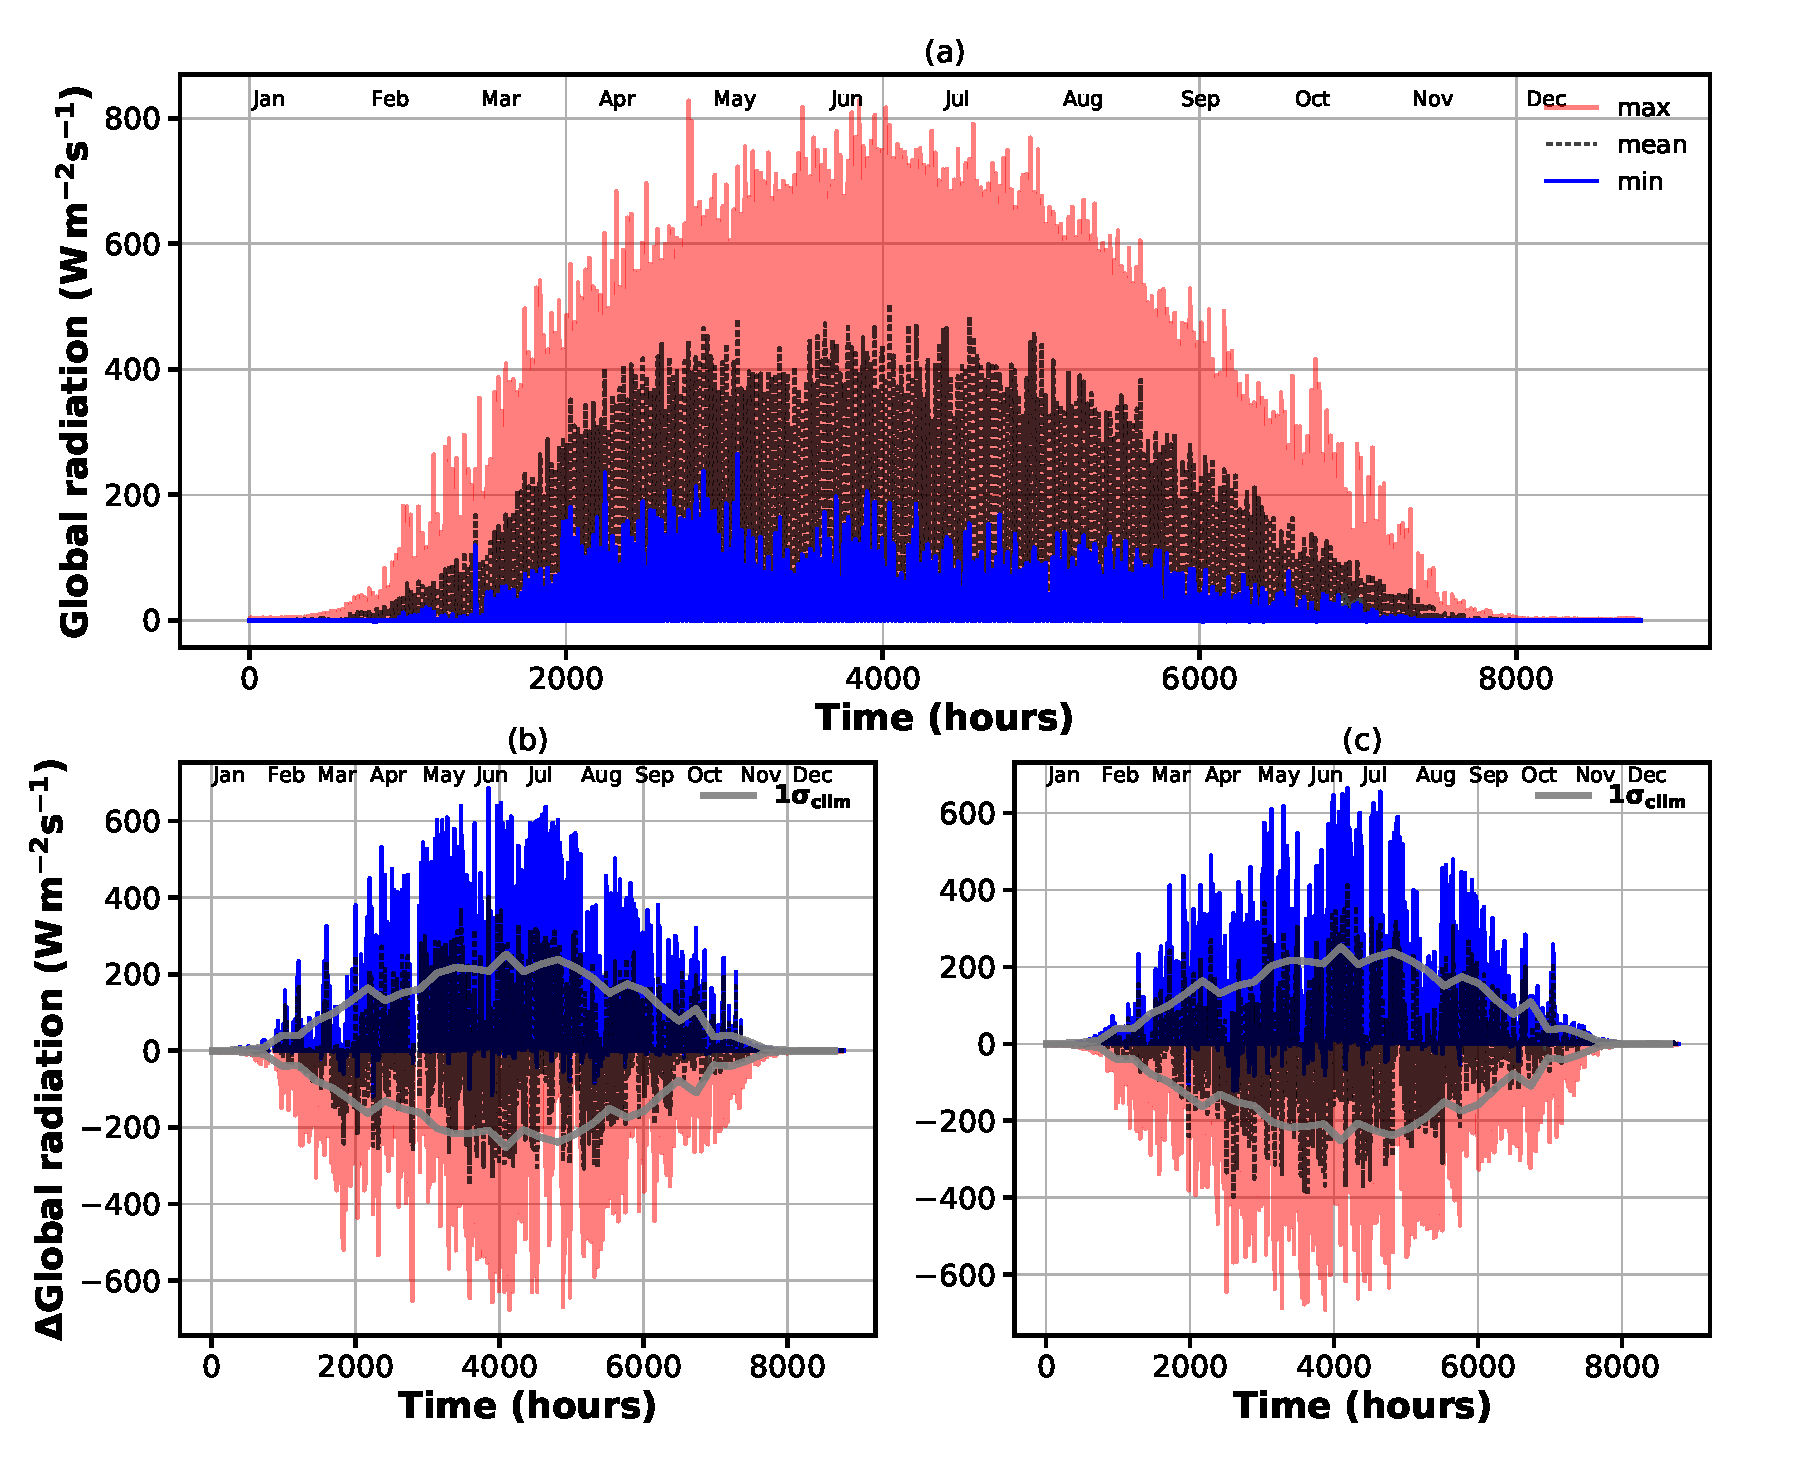
\includegraphics[width=12cm]{global_rad_clim}
  \caption{Observed global irradiance at Svanvik. The cyan lines indicate the $1\,\sigma$ level deducted from the climatology. (a) Climatology (hourly maxima, mean, and minima); deviation from climatology (b) 2018; (c) 2019.}
  \label{fig:global_rad_clim}
\end{figure*}

\begin{figure*}[t]
  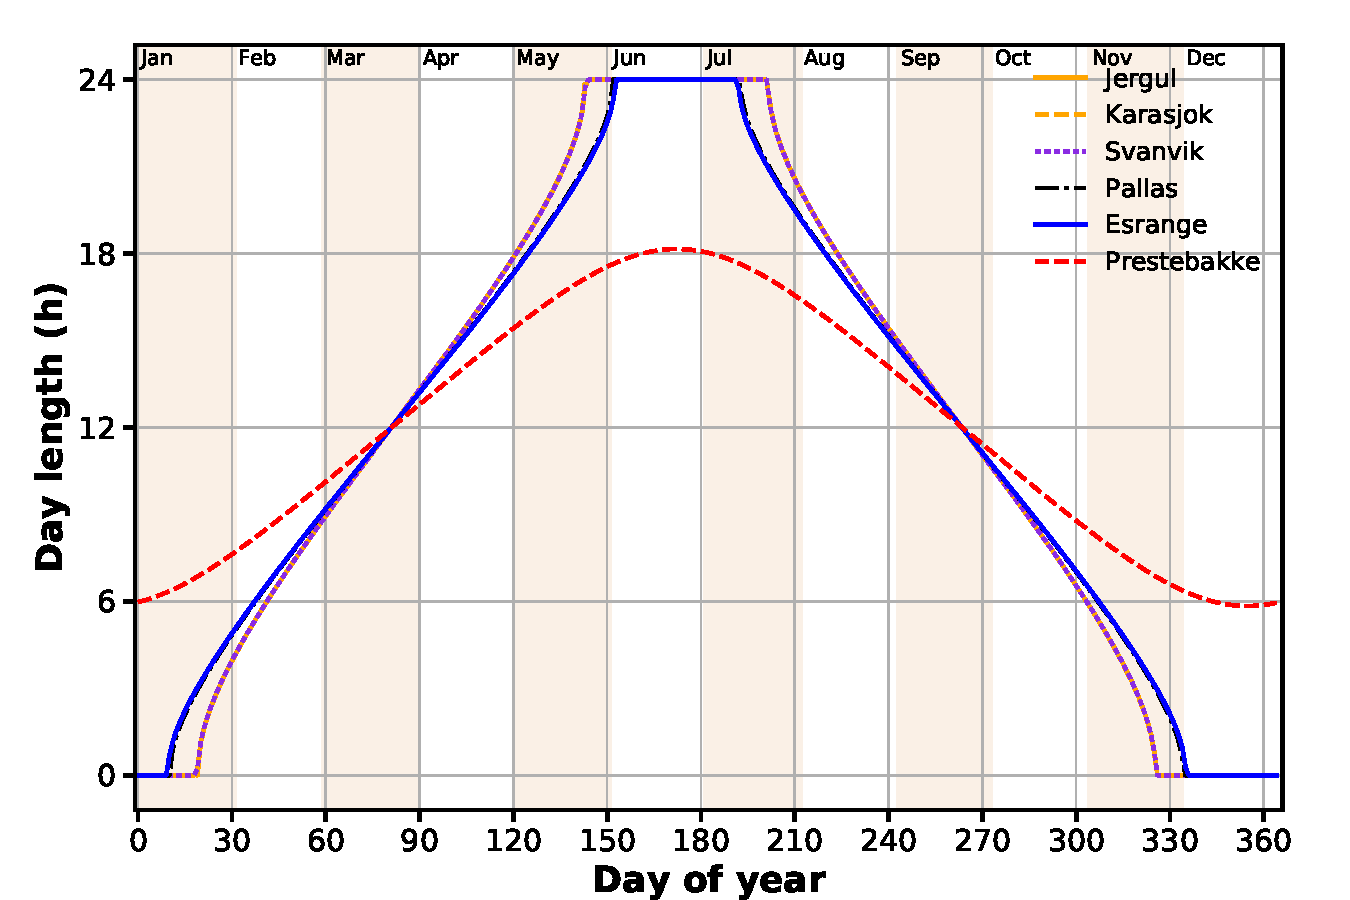
\includegraphics[width=12cm]{test_fennoscandia}
  \caption{Maximum daily sun shine duration based on geometrical calculations at different sites in Fennoscandia. Midnight sun conditions at Jergul/Karasjok and Svanvik prevail from the end of May until the end of July, while at Esrange and Pallas they only prevail from the beginning of June until mid of July.}
  \label{fig:sunlight_fennoscandia}
\end{figure*}

\begin{figure*}[t]
  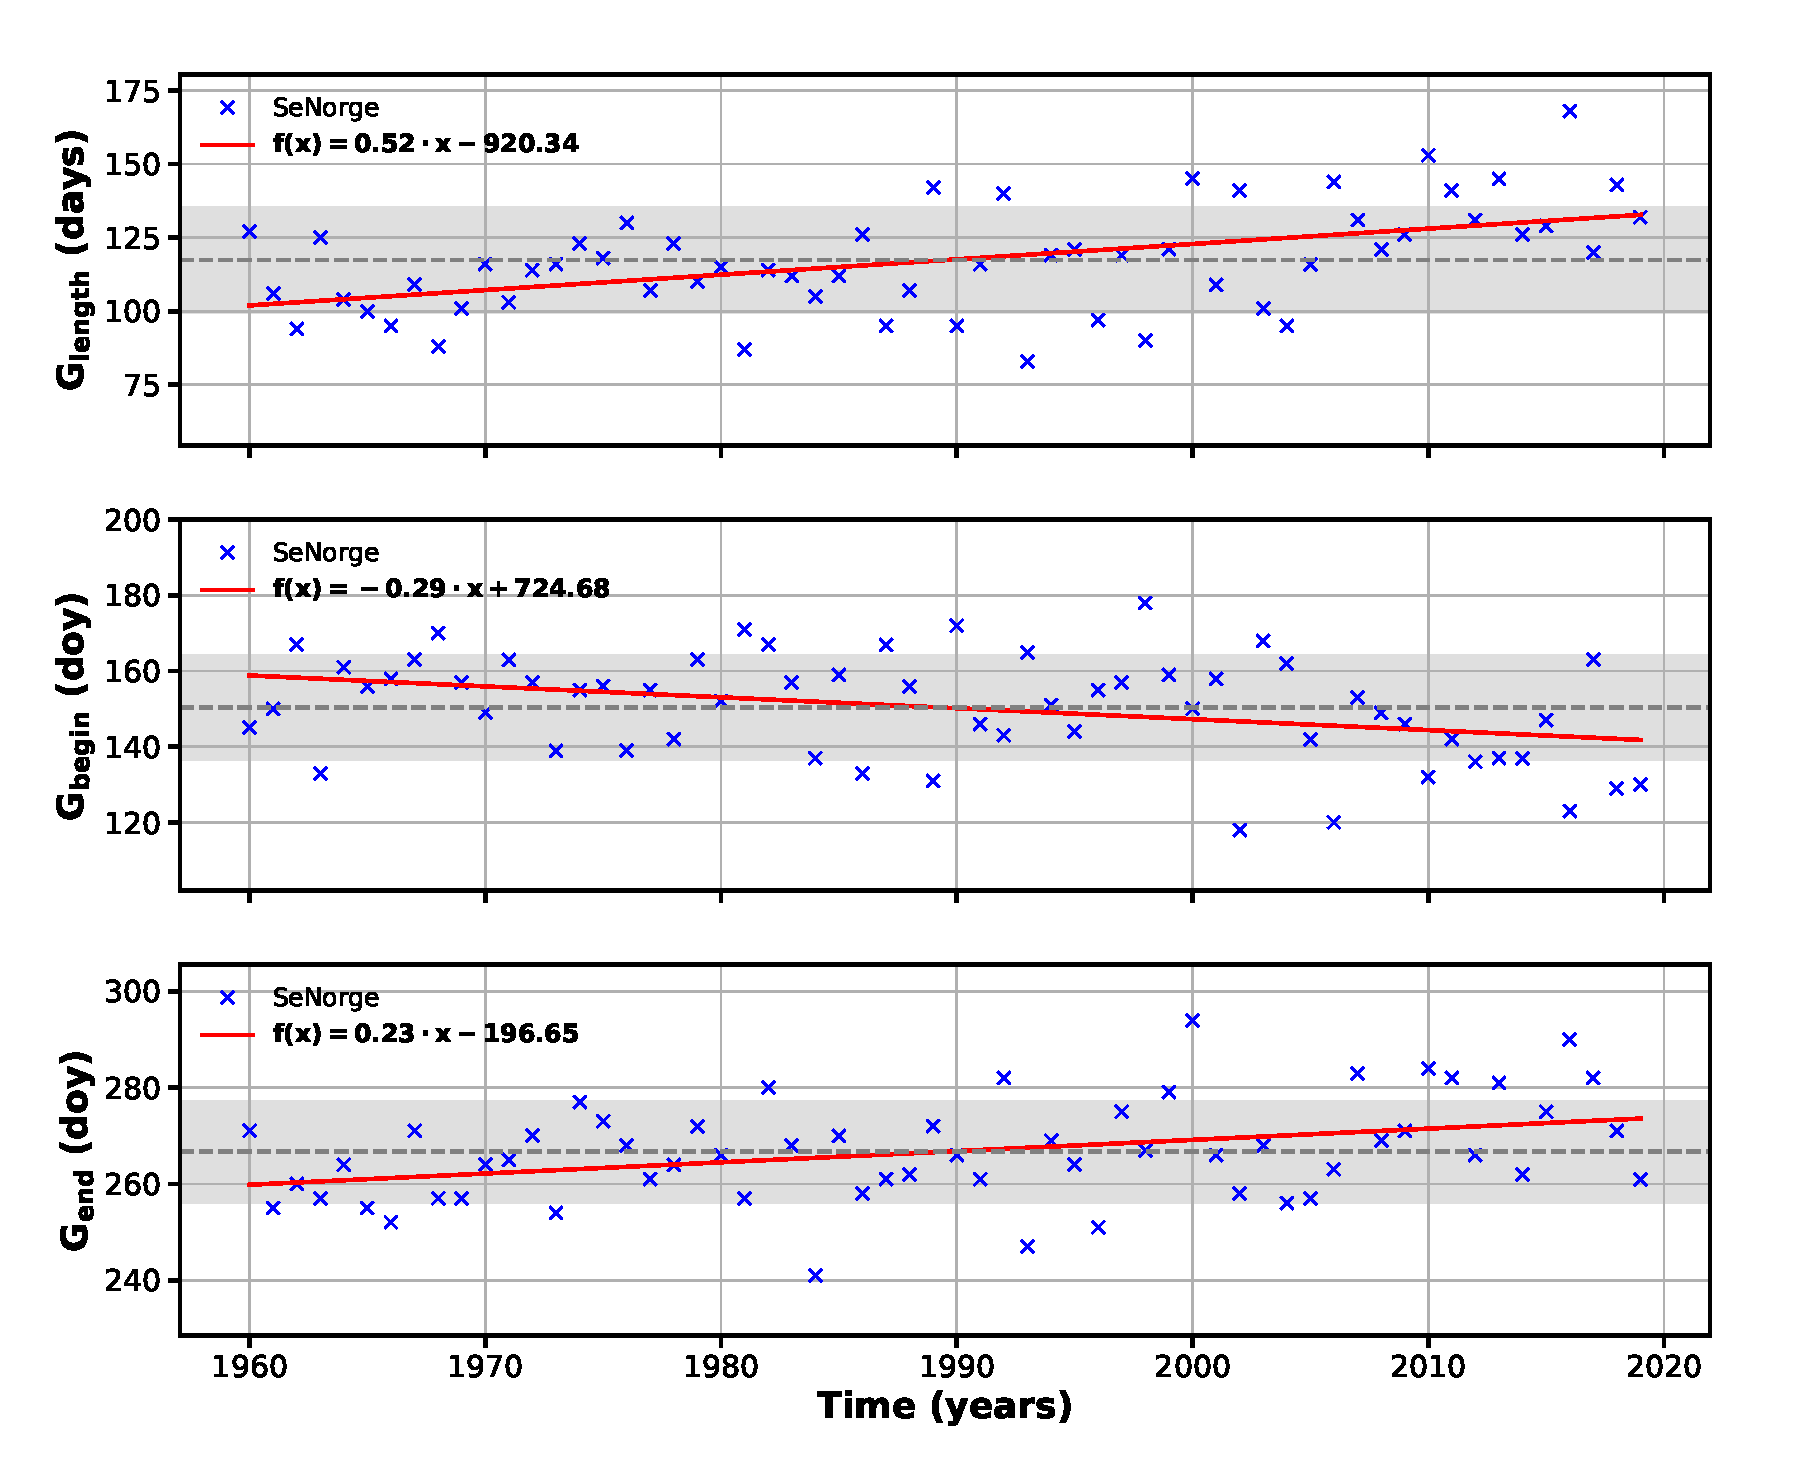
\includegraphics[width=12cm]{greening_season_change_Svanvik}
  \caption{Estimated shift and prolongation of greening season at Svanhovd over the past 6 decades based on data from SeNorge.no {\bf TODO: citation http://www.senorge.no}.}
  \label{fig:greening_season_change_Svanvik}
\end{figure*}
\clearpage


\subsection{Ozone}

\begin{figure*}[t]
  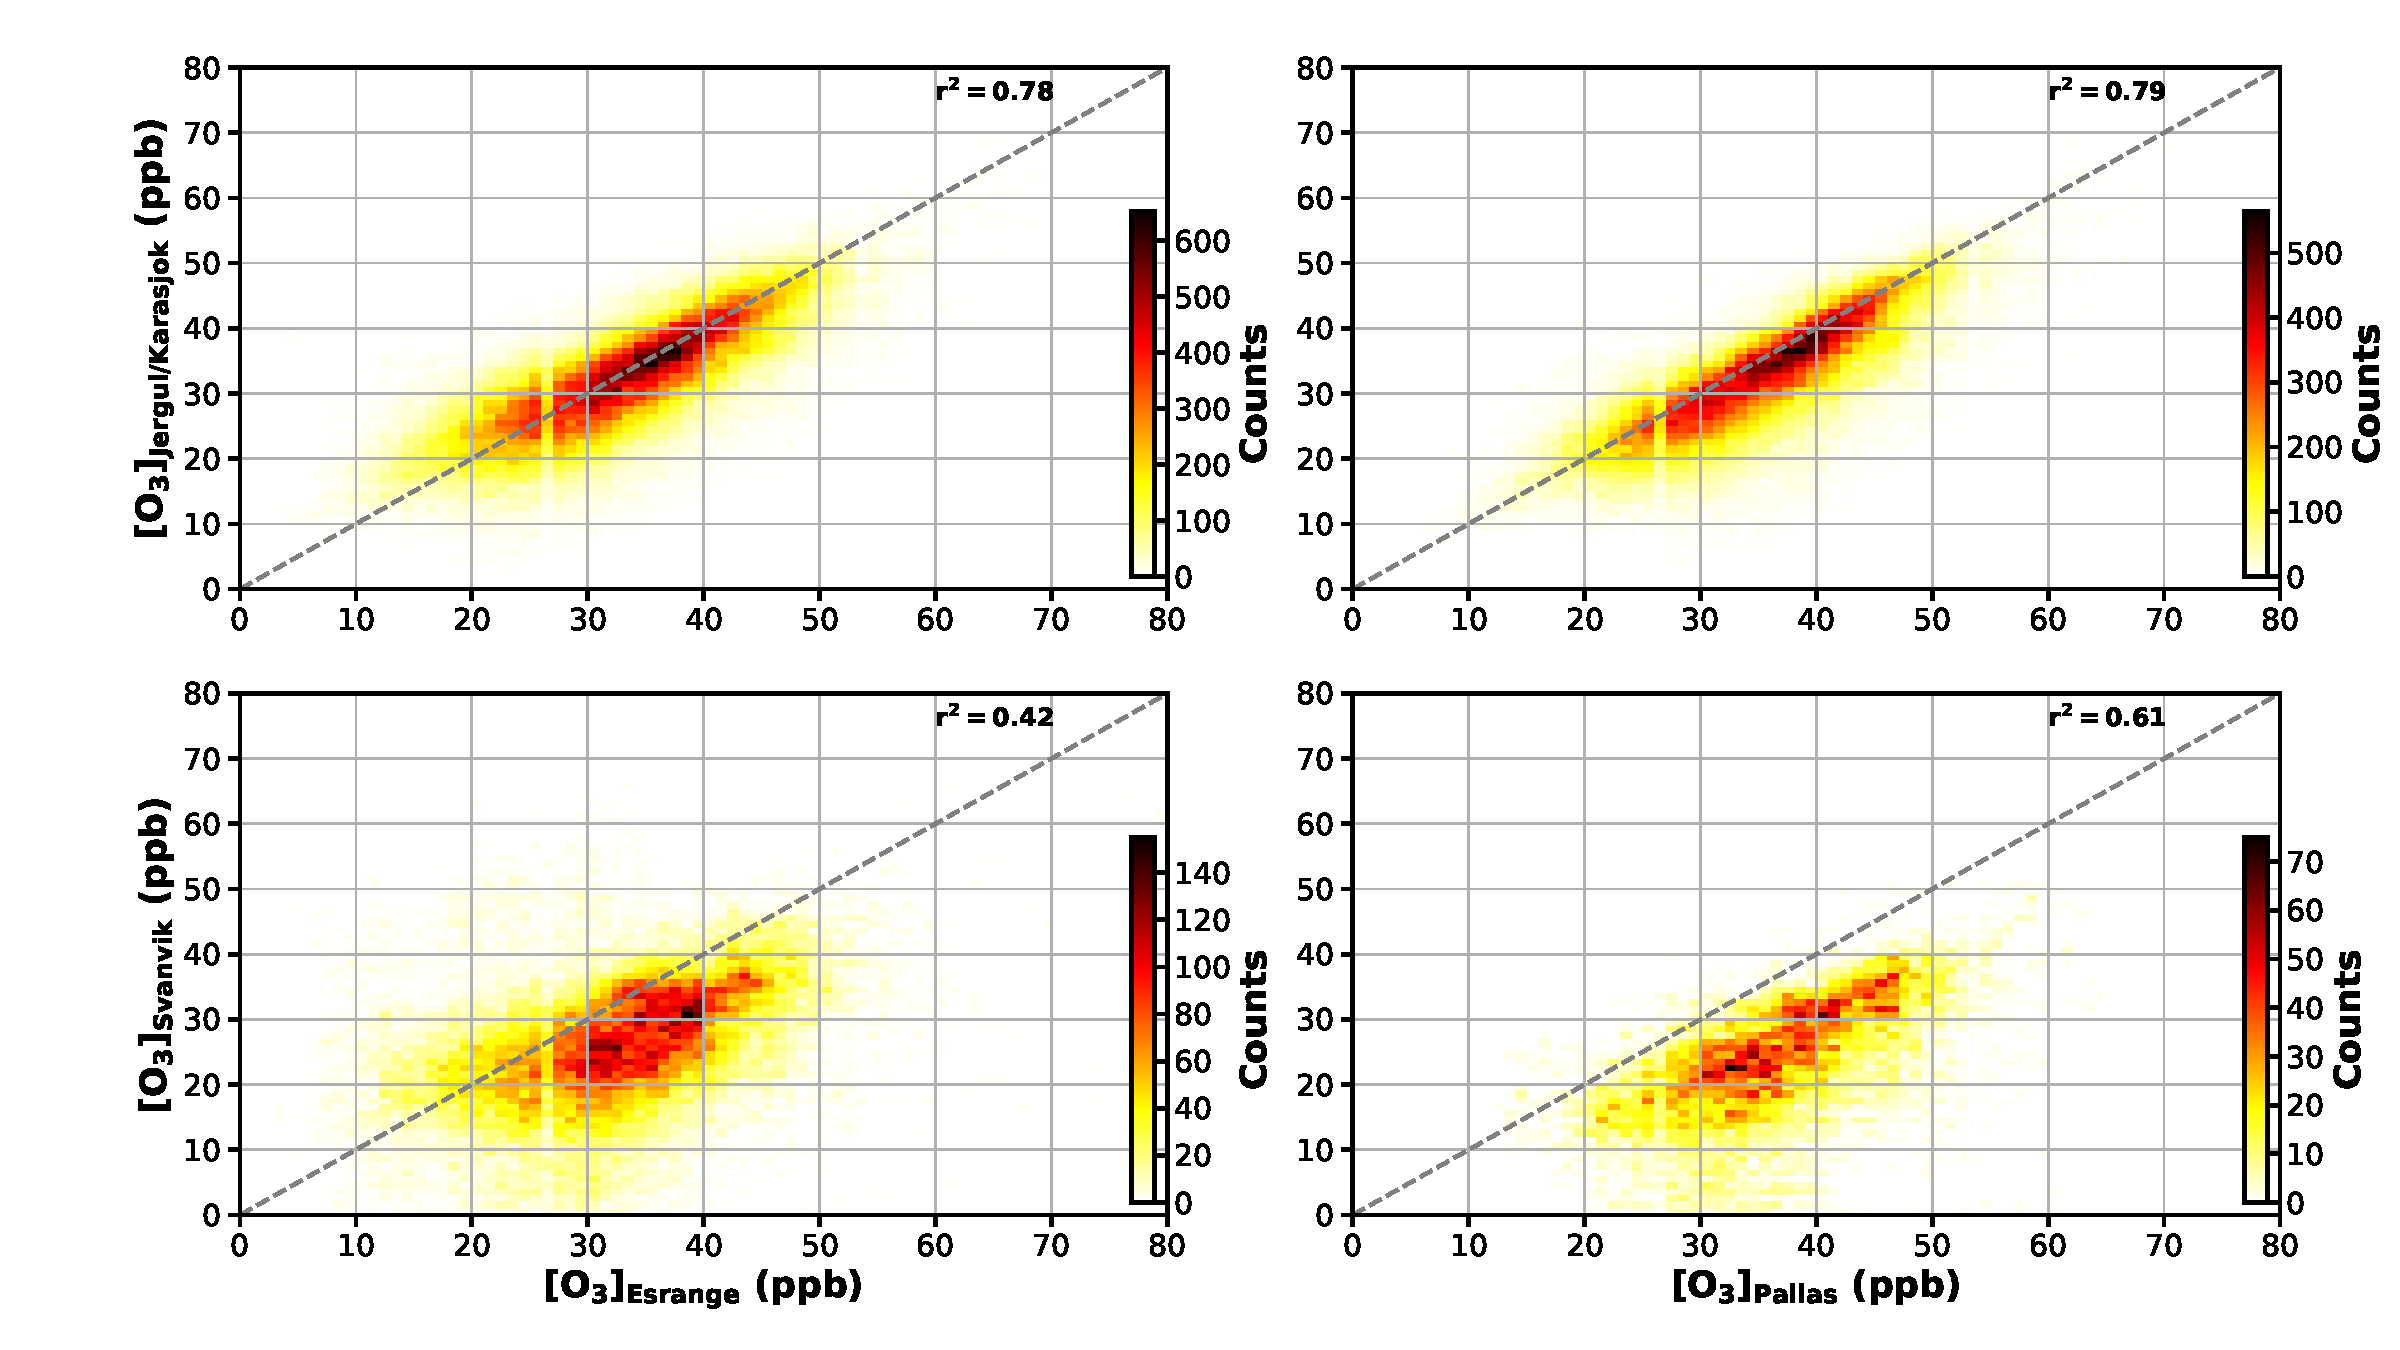
\includegraphics[width=12cm]{density_distribution}
  \caption{Probability densities and correlation coefficient for \chem{[O_3]} between different sites in northern Fennoscandia. Jergul/Karasjok is well correlated with Esrange, and Pallas. Svanvik displays highest correlation with Pallas. (a) Jergul/Karasjok--Esrange; (b) Jergul/Karasjok--Pallas; (c) Svanvik--Esrange; (d) Svanvik--Pallas.}
  \label{fig:density_distribution}
\end{figure*}

\begin{figure*}[t]
  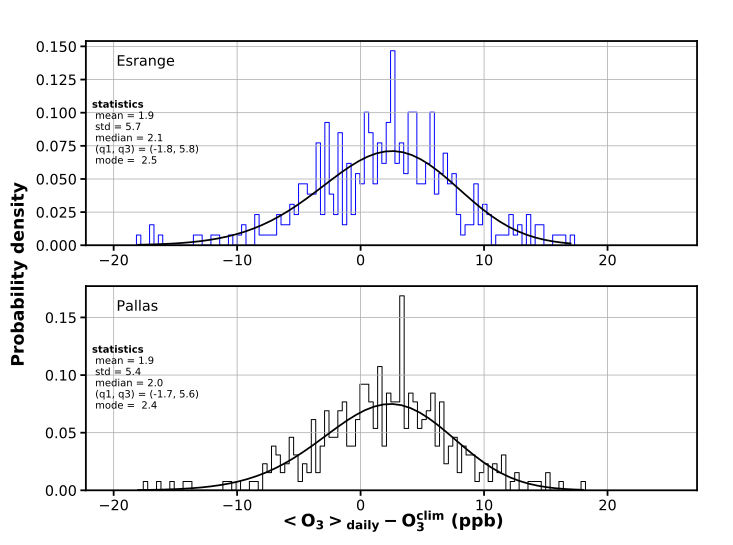
\includegraphics[width=12cm]{ozone_climatology_fenoscandic_obs_residuals}
  \caption{Probability density functions of ozone concentration residuals. 2018 with respect to respective climatology for different sites in Fennoscandia. (a) Esrange; (b) Pallas.}
  \label{fig:ozone_climatology_fenoscandic_obs_residuals}
\end{figure*}

\begin{figure*}[t]
  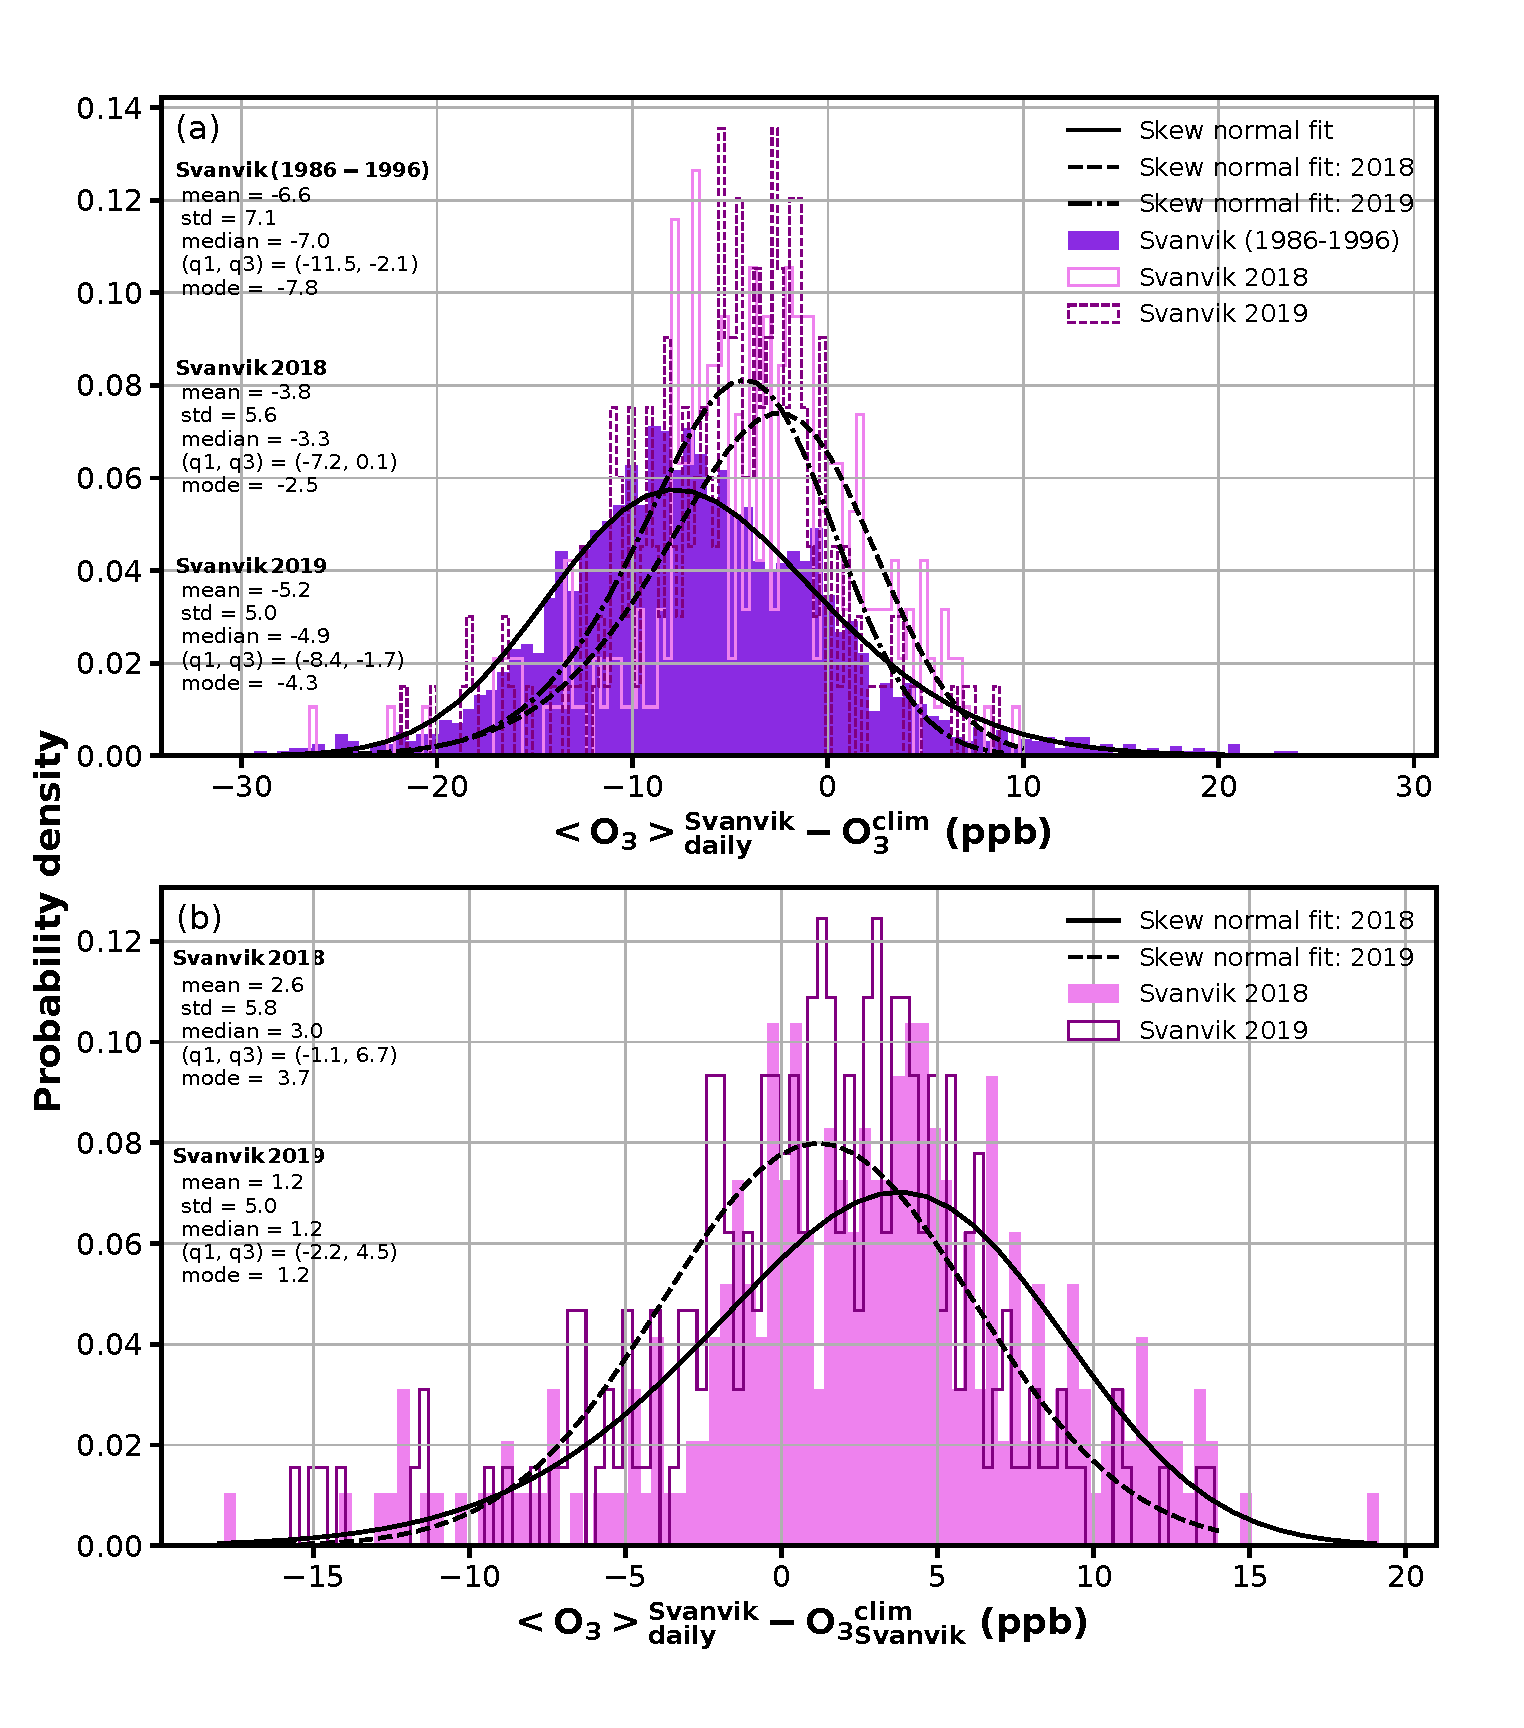
\includegraphics[width=12cm]{ozone_climatology_fenoscandic_obs_residuals-Svanvik}
  \caption{Probability density functions of ozone concentration residuals. 2018/19 observations at Svanhovd with respect to derived climatologies for (a) Northern Fennoscandia; (b) Svanvik.}
  \label{fig:ozone_climatology_fenoscandic_obs_residuals-Svanvik}
\end{figure*}

\begin{figure*}[t]
  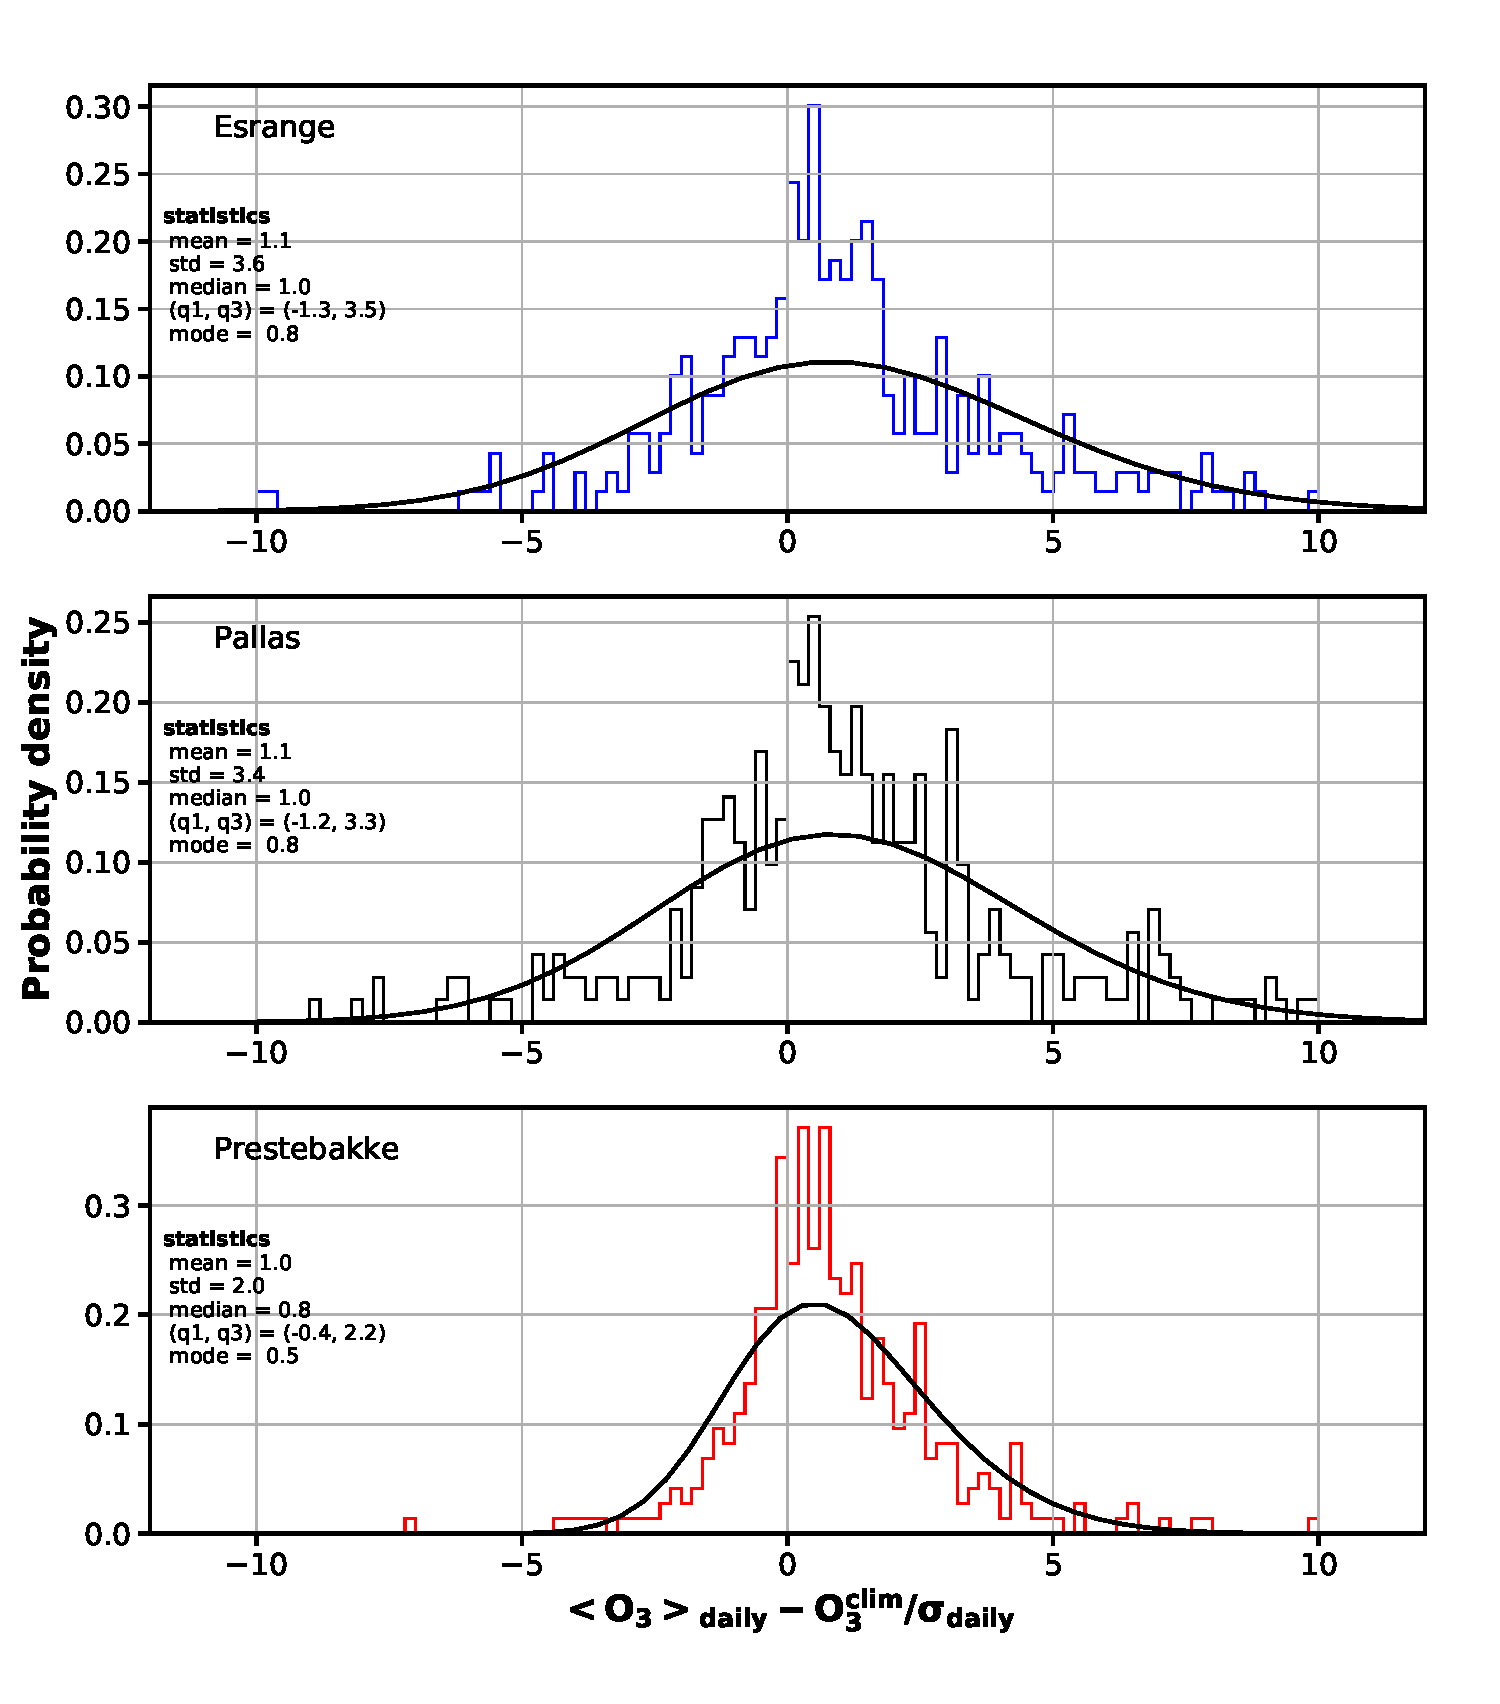
\includegraphics[width=12cm]{ozone_climatology_fenoscandic_obs_test}
  \caption{Student's t-test assuming same sample uncertainty in both, climatology and 2018 observations for different sites in Fennoscandia. \chem{\Delta[O_3]} in Fig.~\ref{fig:ozone_climatology_fenoscandic_obs_residuals} are significantly different from zero-hypothesis on the $1\,\sigma$ level. (a) Esrange; (b) Pallas.}
  \label{fig:ozone_climatology_fenoscandic_obs_test}
\end{figure*}

\begin{figure*}[t]
  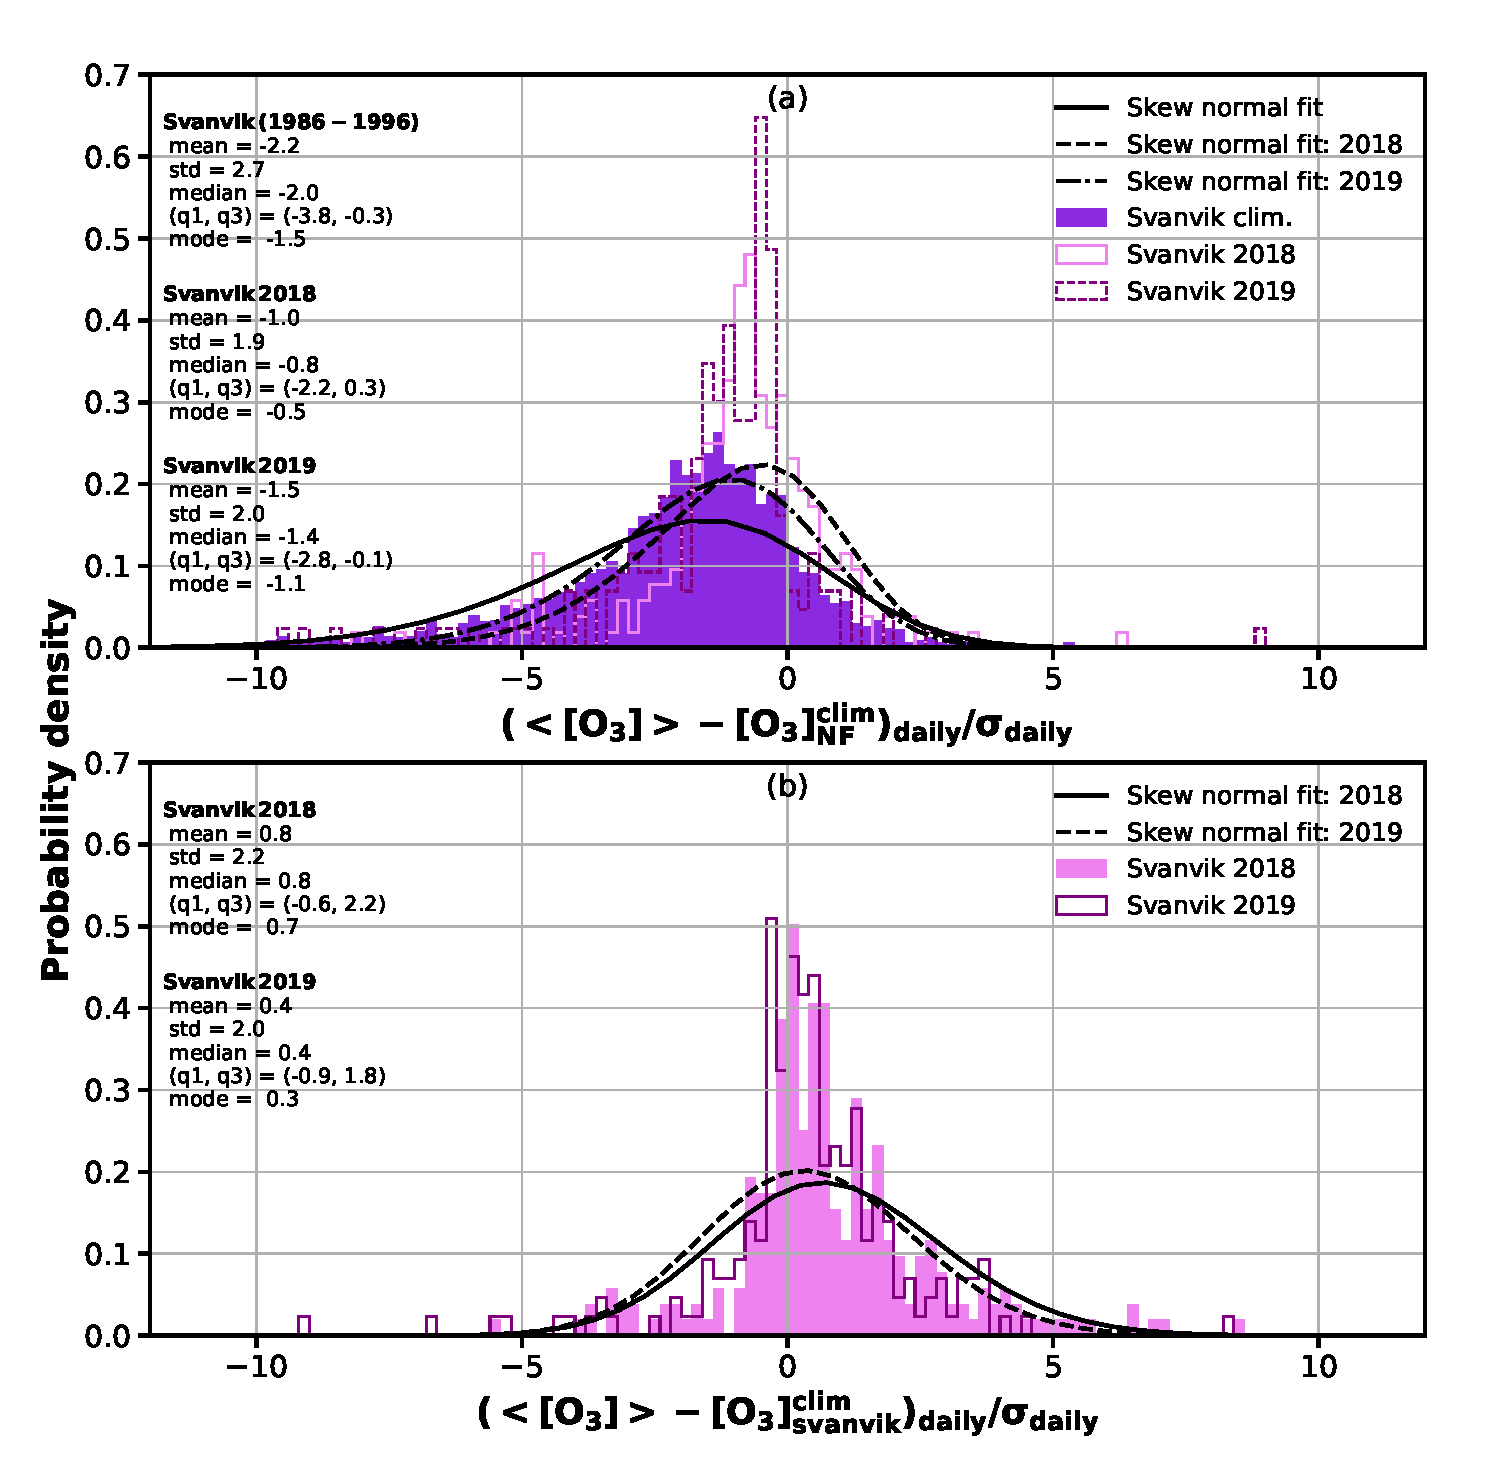
\includegraphics[width=12cm]{ozone_climatology_fenoscandic_obs_test-Svanvik}
  \caption{Student's t-test assuming same sample uncertainty in both, climatology and 2018/19 observations at Svanhovd with respect to derived climatologies for (a) Northern Fennoscandia; (b) Svanvik. \chem{\Delta[O_3]} in Fig.~\ref{fig:ozone_climatology_fenoscandic_obs_residuals}a) are significantly different from zero-hypothesis on the $2\,\sigma$,  $1\,\sigma$ level, respectively. \chem{\Delta[O_3]} in Fig.~\ref{fig:ozone_climatology_fenoscandic_obs_residuals}b) are not significantly different from zero-hypothesis.}
  \label{fig:ozone_climatology_fenoscandic_obs_test-Svanvik}
\end{figure*}

\begin{figure*}[t]
  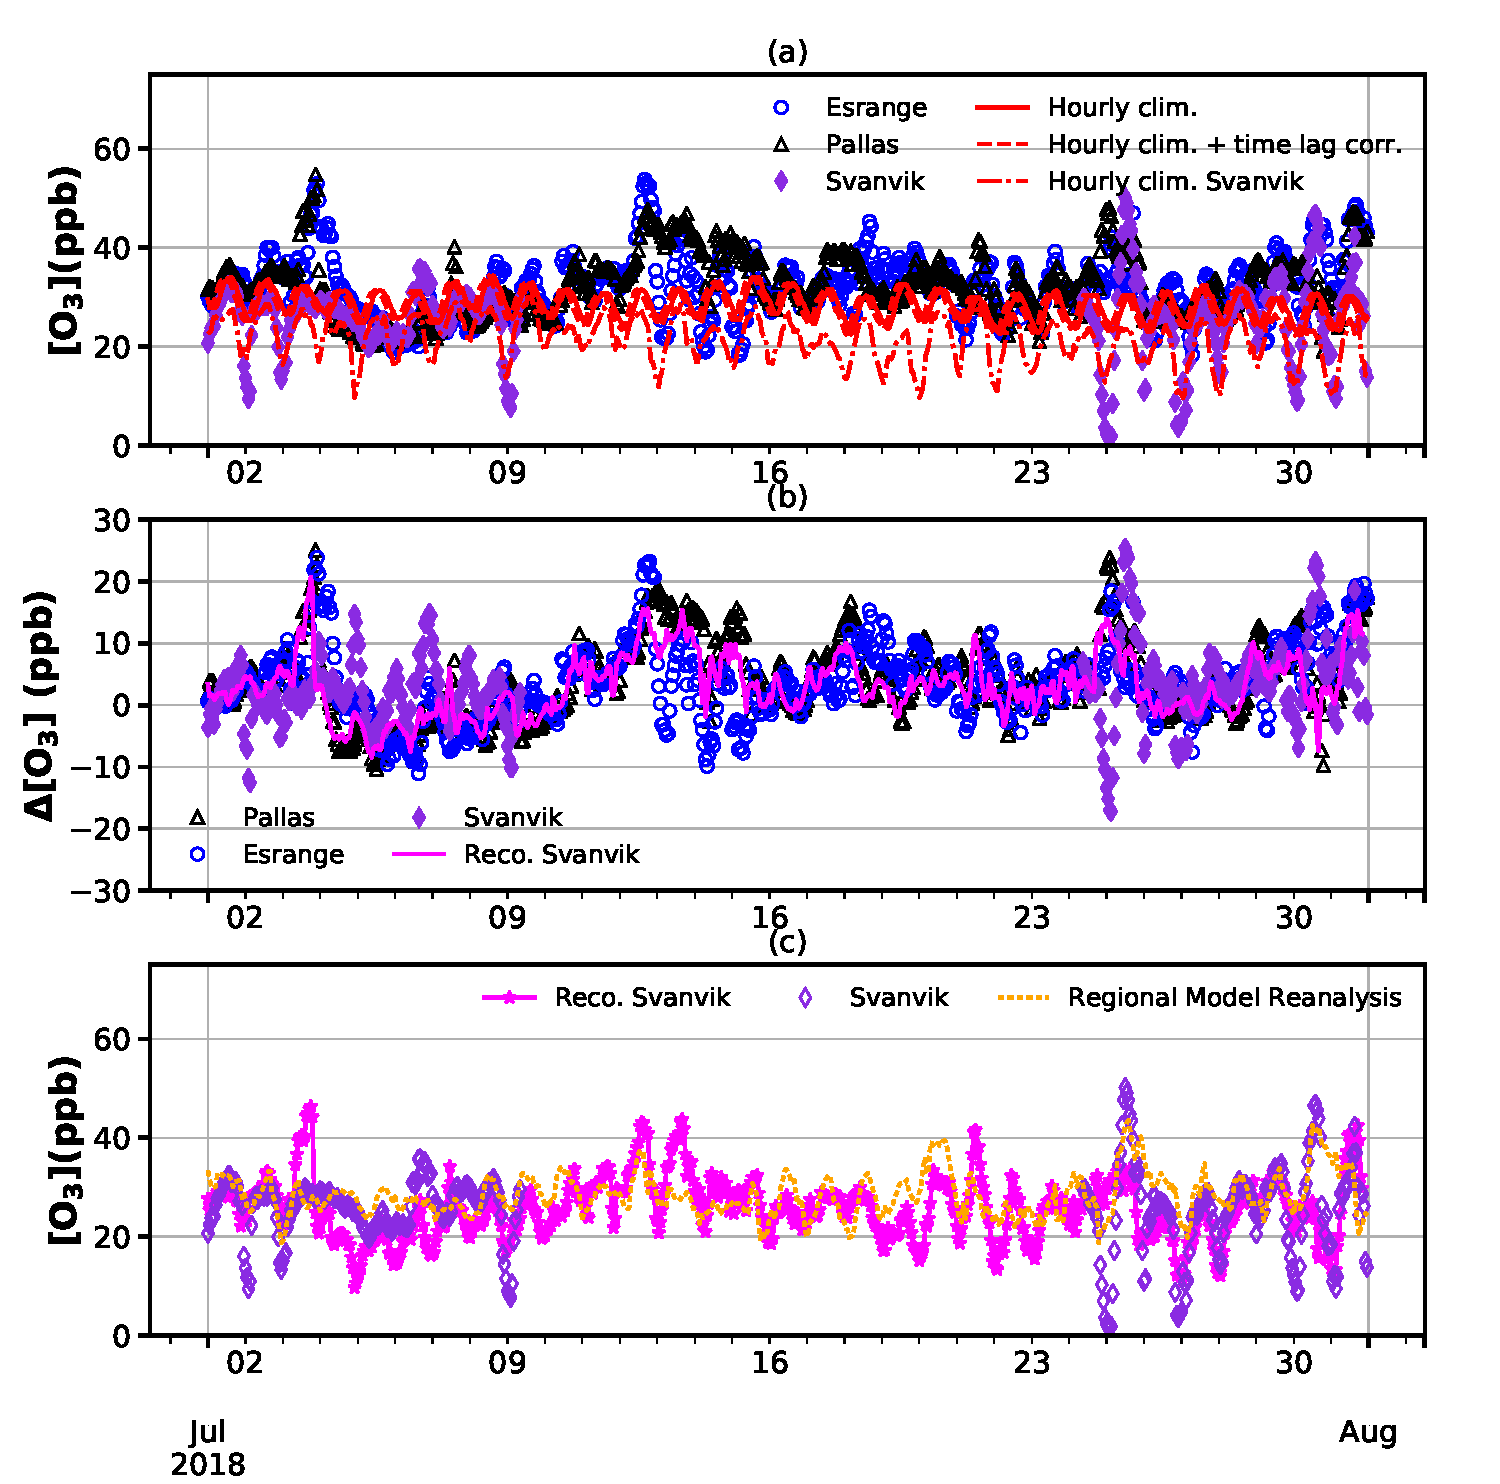
\includegraphics[width=12cm]{ozone_reconstruction_2018_07}
  \caption{Reconstruction of missing \chem{[O_3]} observation data at Svanvik in July 2018 based on derived hourly climatologies of northern Fennoscandia, Svanvik, and data Pallas. (a) Time series; (b) anomalies; (c) reconstruction.}
  \label{fig:ozone_reconstruction_2018_07}
\end{figure*}

\begin{figure*}[t]
  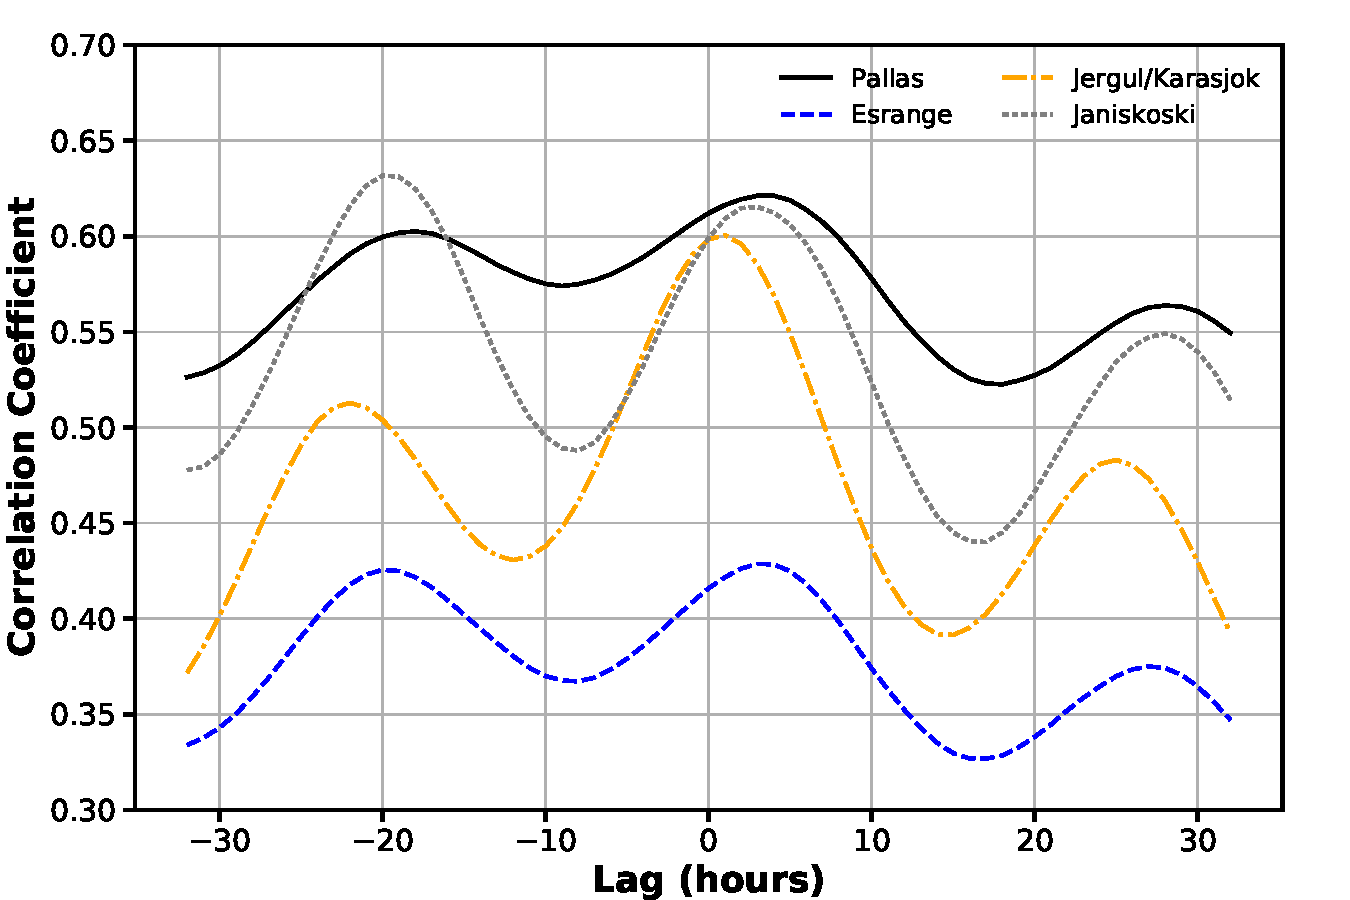
\includegraphics[width=12cm]{ozone_observation_timelag_svanvik}
  \caption{Temporal correlation of \chem{[O_3]} data at Svanvik with other ozone monitoring stations in northern Fennoscandia. A negative lag means that Svanvik lags behind, while a positive lag mean the other station lags behind. The highest correlation with Pallas/Esrange is found at a time lag of $3\,\unit{h}$, for Jergul/Karasjok at $1\,\unit{h}$, and for Janiskoski at $-20\,\unit{h}$.}
  \label{fig:time_lag_correlation}
\end{figure*}

% Shall go to supplement!
\begin{figure*}[t]
  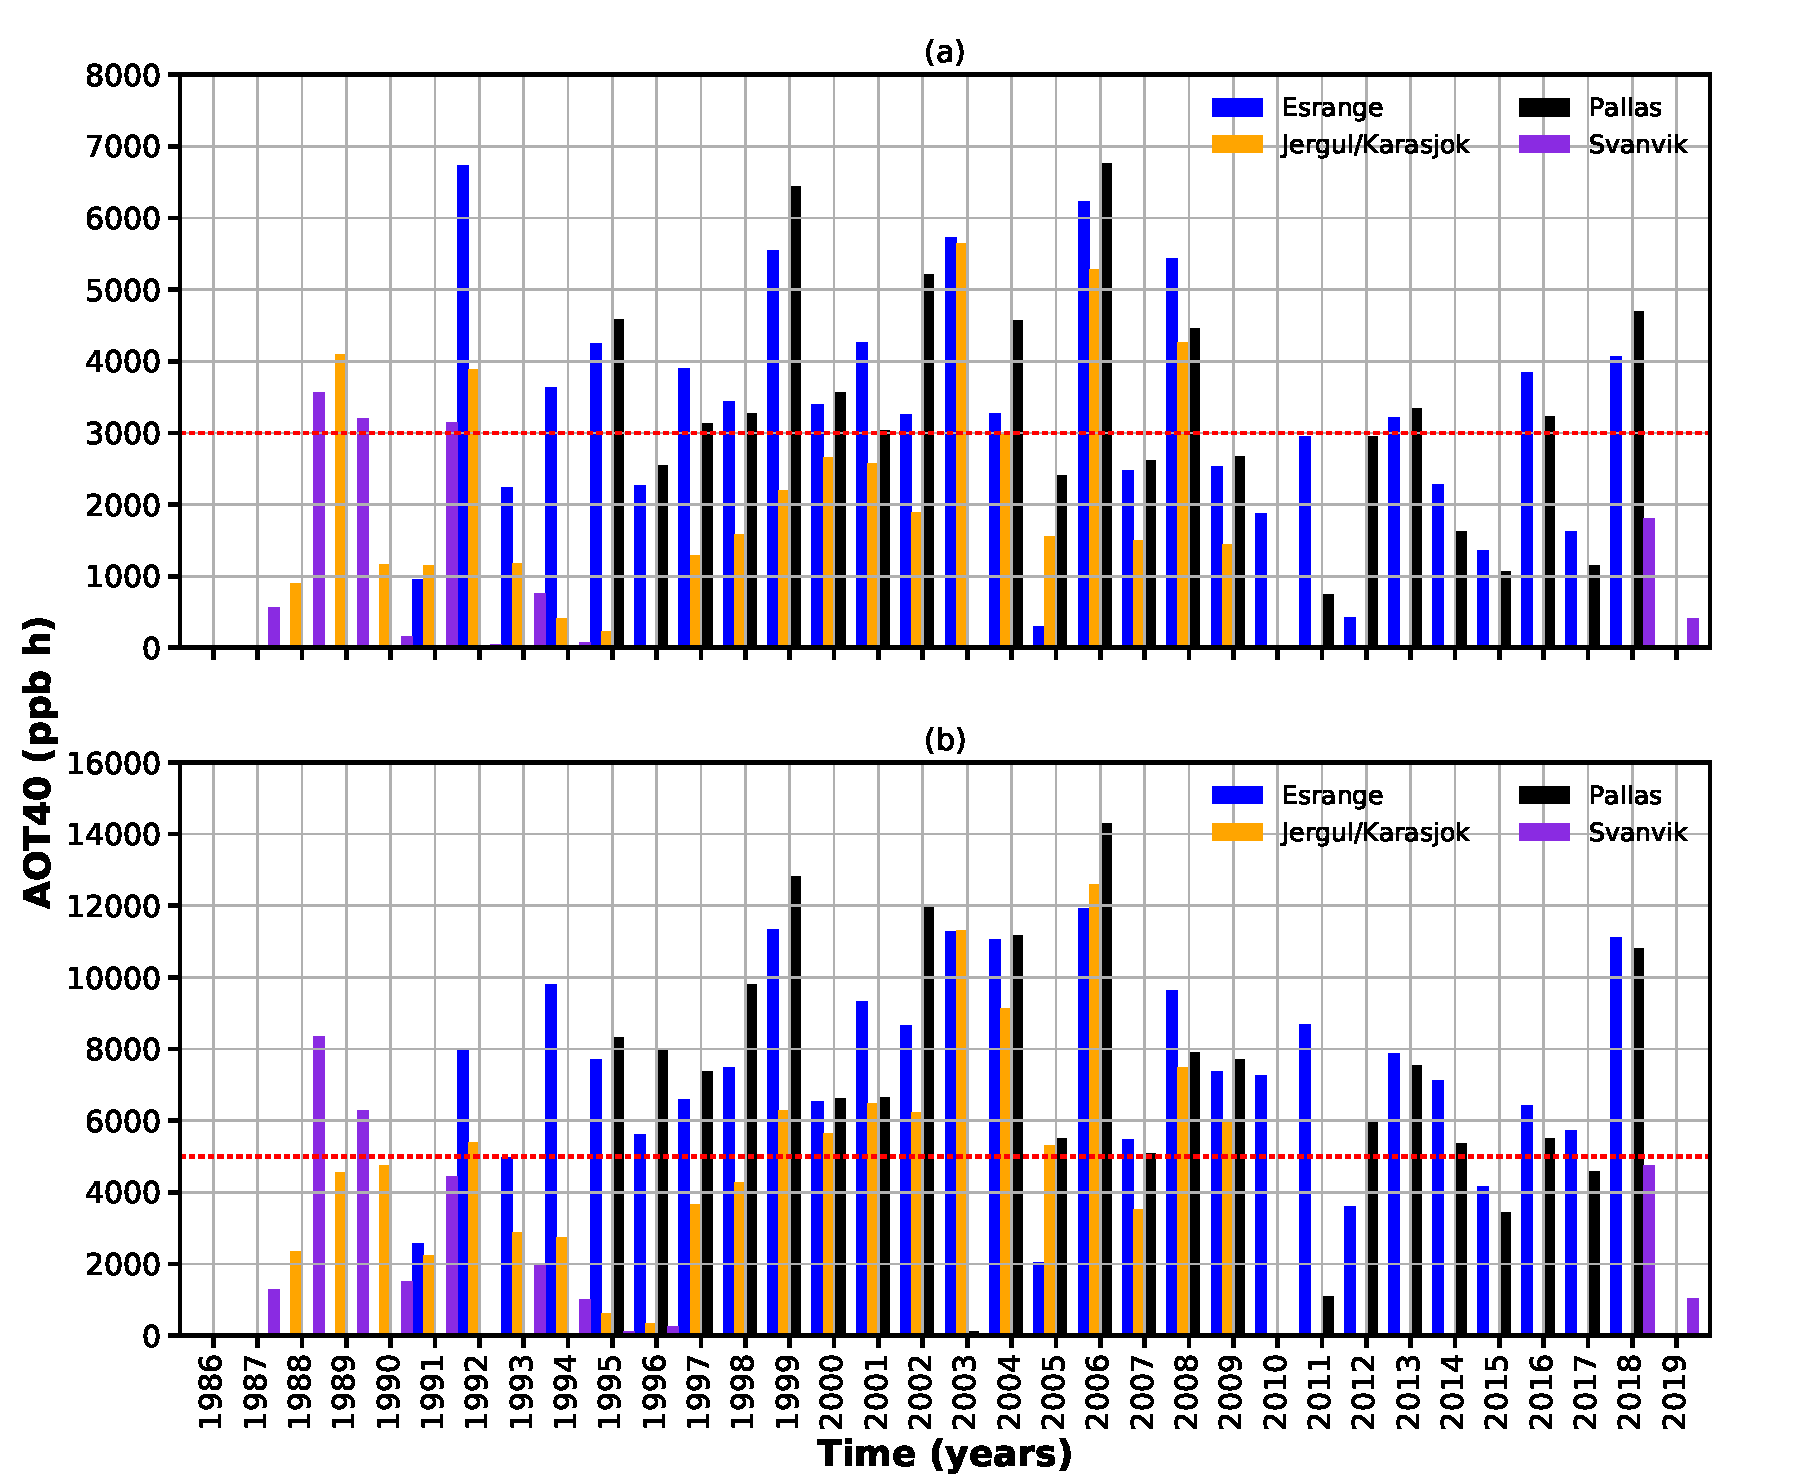
\includegraphics[width=12cm]{ozone_fennoscandic_obs_aot40}
  \caption{Integrated AOT40 for various sites in northern Fennoscandia over the course of 33 years. For simplicity, we integrated hourly ozone between $1\,\unit{am}-11\,\unit{pm}$ in any case, although a night time light intensity $> 50\,\unit{W\,m^{-2}}$ is only measured during midnight sun conditions. Since night time \chem{[O_3]} is mostly below $40\,\unit{ppb}$, the such induced high bias in spring should be tolerable. The dashed red lines indicate the respective threshold given by the EU directive. (a) May 1 -- July 31 (b) April 1 -- September 30.}
  \label{fig:fennoscandic_aot40}
\end{figure*}

\clearpage

\noappendix       %% use this to mark the end of the appendix section. Otherwise the figures might be numbered incorrectly (e.g. 10 instead of 1).

%% Regarding figures and tables in appendices, the following two options are possible depending on your general handling of figures and tables in the manuscript environment:

%% Option 1: If you sorted all figures and tables into the sections of the text, please also sort the appendix figures and appendix tables into the respective appendix sections.
%% They will be correctly named automatically.

%% Option 2: If you put all figures after the reference list, please insert appendix tables and figures after the normal tables and figures.
%% To rename them correctly to A1, A2, etc., please add the following commands in front of them:

%\appendixfigures  %% needs to be added in front of appendix figures


%\noappendix

%\appendixtables   %% needs to be added in front of appendix tables

%% Please add \clearpage between each table and/or figure. Further guidelines on figures and tables can be found below.



\authorcontribution{TEXT} %% this section is mandatory

\competinginterests{TEXT} %% this section is mandatory even if you declare that no competing interests are present

\disclaimer{TEXT} %% optional section

\begin{acknowledgements}
TEXT
\end{acknowledgements}




%% REFERENCES

%% The reference list is compiled as follows:

%\begin{thebibliography}{}

%\bibitem[AUTHOR(YEAR)]{LABEL1}
%REFERENCE 1

%\bibitem[AUTHOR(YEAR)]{LABEL2}
%REFERENCE 2

%\end{thebibliography}

%% Since the Copernicus LaTeX package includes the BibTeX style file copernicus.bst,
%% authors experienced with BibTeX only have to include the following two lines:
%%
\bibliographystyle{copernicus}
\bibliography{VegOzone.bib}
%%
%% URLs and DOIs can be entered in your BibTeX file as:
%%
%% URL = {http://www.xyz.org/~jones/idx_g.htm}
%% DOI = {10.5194/xyz}


%% LITERATURE CITATIONS
%%
%% command                        & example result
%% \citet{jones90}|               & Jones et al. (1990)
%% \citep{jones90}|               & (Jones et al., 1990)
%% \citep{jones90,jones93}|       & (Jones et al., 1990, 1993)
%% \citep[p.~32]{jones90}|        & (Jones et al., 1990, p.~32)
%% \citep[e.g.,][]{jones90}|      & (e.g., Jones et al., 1990)
%% \citep[e.g.,][p.~32]{jones90}| & (e.g., Jones et al., 1990, p.~32)
%% \citeauthor{jones90}|          & Jones et al.
%% \citeyear{jones90}|            & 1990



%% FIGURES

%% When figures and tables are placed at the end of the MS (article in one-column style), please add \clearpage
%% between bibliography and first table and/or figure as well as between each table and/or figure.

% The figure files should be labelled correctly with Arabic numerals (e.g. fig01.jpg, fig02.png).


%% ONE-COLUMN FIGURES

%%f
%\begin{figure}[t]
%\includegraphics[width=8.3cm]{FILE NAME}
%\caption{TEXT}
%\end{figure}
%
%%% TWO-COLUMN FIGURES
%
%%f
%\begin{figure*}[t]
%\includegraphics[width=12cm]{FILE NAME}
%\caption{TEXT}
%\end{figure*}
%
%
%%% TABLES
%%%
%%% The different columns must be seperated with a & command and should
%%% end with \\ to identify the column brake.
%
%%% ONE-COLUMN TABLE
%
%%t
%\begin{table}[t]
%\caption{TEXT}
%\begin{tabular}{column = lcr}
%\tophline
%
%\middlehline
%
%\bottomhline
%\end{tabular}
%\belowtable{} % Table Footnotes
%\end{table}
%
%%% TWO-COLUMN TABLE
%
%%t
%\begin{table*}[t]
%\caption{TEXT}
%\begin{tabular}{column = lcr}
%\tophline
%
%\middlehline
%
%\bottomhline
%\end{tabular}
%\belowtable{} % Table Footnotes
%\end{table*}
%
%%% LANDSCAPE TABLE
%
%%t
%\begin{sidewaystable*}[t]
%\caption{TEXT}
%\begin{tabular}{column = lcr}
%\tophline
%
%\middlehline
%
%\bottomhline
%\end{tabular}
%\belowtable{} % Table Footnotes
%\end{sidewaystable*}
%
%
%%% MATHEMATICAL EXPRESSIONS
%
%%% All papers typeset by Copernicus Publications follow the math typesetting regulations
%%% given by the IUPAC Green Book (IUPAC: Quantities, Units and Symbols in Physical Chemistry,
%%% 2nd Edn., Blackwell Science, available at: http://old.iupac.org/publications/books/gbook/green_book_2ed.pdf, 1993).
%%%
%%% Physical quantities/variables are typeset in italic font (t for time, T for Temperature)
%%% Indices which are not defined are typeset in italic font (x, y, z, a, b, c)
%%% Items/objects which are defined are typeset in roman font (Car A, Car B)
%%% Descriptions/specifications which are defined by itself are typeset in roman font (abs, rel, ref, tot, net, ice)
%%% Abbreviations from 2 letters are typeset in roman font (RH, LAI)
%%% Vectors are identified in bold italic font using \vec{x}
%%% Matrices are identified in bold roman font
%%% Multiplication signs are typeset using the LaTeX commands \times (for vector products, grids, and exponential notations) or \cdot
%%% The character * should not be applied as mutliplication sign
%
%
%%% EQUATIONS
%
%%% Single-row equation
%
%\begin{equation}
%
%\end{equation}
%
%%% Multiline equation
%
%\begin{align}
%& 3 + 5 = 8\\
%& 3 + 5 = 8\\
%& 3 + 5 = 8
%\end{align}
%
%
%%% MATRICES
%
%\begin{matrix}
%x & y & z\\
%x & y & z\\
%x & y & z\\
%\end{matrix}
%
%
%%% ALGORITHM
%
%\begin{algorithm}
%\caption{...}
%\label{a1}
%\begin{algorithmic}
%...
%\end{algorithmic}
%\end{algorithm}
%
%
%%% CHEMICAL FORMULAS AND REACTIONS
%
%%% For formulas embedded in the text, please use \chem{}
%
%%% The reaction environment creates labels including the letter R, i.e. (R1), (R2), etc.
%
%\begin{reaction}
%%% \rightarrow should be used for normal (one-way) chemical reactions
%%% \rightleftharpoons should be used for equilibria
%%% \leftrightarrow should be used for resonance structures
%\end{reaction}
%
%
%%% PHYSICAL UNITS
%%%
%%% Please use \unit{} and apply the exponential notation


\end{document}
